% Options for packages loaded elsewhere
\PassOptionsToPackage{unicode}{hyperref}
\PassOptionsToPackage{hyphens}{url}
%
\documentclass[
]{book}
\usepackage{amsmath,amssymb}
\usepackage{iftex}
\ifPDFTeX
  \usepackage[T1]{fontenc}
  \usepackage[utf8]{inputenc}
  \usepackage{textcomp} % provide euro and other symbols
\else % if luatex or xetex
  \usepackage{unicode-math} % this also loads fontspec
  \defaultfontfeatures{Scale=MatchLowercase}
  \defaultfontfeatures[\rmfamily]{Ligatures=TeX,Scale=1}
\fi
\usepackage{lmodern}
\ifPDFTeX\else
  % xetex/luatex font selection
\fi
% Use upquote if available, for straight quotes in verbatim environments
\IfFileExists{upquote.sty}{\usepackage{upquote}}{}
\IfFileExists{microtype.sty}{% use microtype if available
  \usepackage[]{microtype}
  \UseMicrotypeSet[protrusion]{basicmath} % disable protrusion for tt fonts
}{}
\makeatletter
\@ifundefined{KOMAClassName}{% if non-KOMA class
  \IfFileExists{parskip.sty}{%
    \usepackage{parskip}
  }{% else
    \setlength{\parindent}{0pt}
    \setlength{\parskip}{6pt plus 2pt minus 1pt}}
}{% if KOMA class
  \KOMAoptions{parskip=half}}
\makeatother
\usepackage{xcolor}
\usepackage{color}
\usepackage{fancyvrb}
\newcommand{\VerbBar}{|}
\newcommand{\VERB}{\Verb[commandchars=\\\{\}]}
\DefineVerbatimEnvironment{Highlighting}{Verbatim}{commandchars=\\\{\}}
% Add ',fontsize=\small' for more characters per line
\usepackage{framed}
\definecolor{shadecolor}{RGB}{248,248,248}
\newenvironment{Shaded}{\begin{snugshade}}{\end{snugshade}}
\newcommand{\AlertTok}[1]{\textcolor[rgb]{0.94,0.16,0.16}{#1}}
\newcommand{\AnnotationTok}[1]{\textcolor[rgb]{0.56,0.35,0.01}{\textbf{\textit{#1}}}}
\newcommand{\AttributeTok}[1]{\textcolor[rgb]{0.13,0.29,0.53}{#1}}
\newcommand{\BaseNTok}[1]{\textcolor[rgb]{0.00,0.00,0.81}{#1}}
\newcommand{\BuiltInTok}[1]{#1}
\newcommand{\CharTok}[1]{\textcolor[rgb]{0.31,0.60,0.02}{#1}}
\newcommand{\CommentTok}[1]{\textcolor[rgb]{0.56,0.35,0.01}{\textit{#1}}}
\newcommand{\CommentVarTok}[1]{\textcolor[rgb]{0.56,0.35,0.01}{\textbf{\textit{#1}}}}
\newcommand{\ConstantTok}[1]{\textcolor[rgb]{0.56,0.35,0.01}{#1}}
\newcommand{\ControlFlowTok}[1]{\textcolor[rgb]{0.13,0.29,0.53}{\textbf{#1}}}
\newcommand{\DataTypeTok}[1]{\textcolor[rgb]{0.13,0.29,0.53}{#1}}
\newcommand{\DecValTok}[1]{\textcolor[rgb]{0.00,0.00,0.81}{#1}}
\newcommand{\DocumentationTok}[1]{\textcolor[rgb]{0.56,0.35,0.01}{\textbf{\textit{#1}}}}
\newcommand{\ErrorTok}[1]{\textcolor[rgb]{0.64,0.00,0.00}{\textbf{#1}}}
\newcommand{\ExtensionTok}[1]{#1}
\newcommand{\FloatTok}[1]{\textcolor[rgb]{0.00,0.00,0.81}{#1}}
\newcommand{\FunctionTok}[1]{\textcolor[rgb]{0.13,0.29,0.53}{\textbf{#1}}}
\newcommand{\ImportTok}[1]{#1}
\newcommand{\InformationTok}[1]{\textcolor[rgb]{0.56,0.35,0.01}{\textbf{\textit{#1}}}}
\newcommand{\KeywordTok}[1]{\textcolor[rgb]{0.13,0.29,0.53}{\textbf{#1}}}
\newcommand{\NormalTok}[1]{#1}
\newcommand{\OperatorTok}[1]{\textcolor[rgb]{0.81,0.36,0.00}{\textbf{#1}}}
\newcommand{\OtherTok}[1]{\textcolor[rgb]{0.56,0.35,0.01}{#1}}
\newcommand{\PreprocessorTok}[1]{\textcolor[rgb]{0.56,0.35,0.01}{\textit{#1}}}
\newcommand{\RegionMarkerTok}[1]{#1}
\newcommand{\SpecialCharTok}[1]{\textcolor[rgb]{0.81,0.36,0.00}{\textbf{#1}}}
\newcommand{\SpecialStringTok}[1]{\textcolor[rgb]{0.31,0.60,0.02}{#1}}
\newcommand{\StringTok}[1]{\textcolor[rgb]{0.31,0.60,0.02}{#1}}
\newcommand{\VariableTok}[1]{\textcolor[rgb]{0.00,0.00,0.00}{#1}}
\newcommand{\VerbatimStringTok}[1]{\textcolor[rgb]{0.31,0.60,0.02}{#1}}
\newcommand{\WarningTok}[1]{\textcolor[rgb]{0.56,0.35,0.01}{\textbf{\textit{#1}}}}
\usepackage{longtable,booktabs,array}
\usepackage{calc} % for calculating minipage widths
% Correct order of tables after \paragraph or \subparagraph
\usepackage{etoolbox}
\makeatletter
\patchcmd\longtable{\par}{\if@noskipsec\mbox{}\fi\par}{}{}
\makeatother
% Allow footnotes in longtable head/foot
\IfFileExists{footnotehyper.sty}{\usepackage{footnotehyper}}{\usepackage{footnote}}
\makesavenoteenv{longtable}
\usepackage{graphicx}
\makeatletter
\def\maxwidth{\ifdim\Gin@nat@width>\linewidth\linewidth\else\Gin@nat@width\fi}
\def\maxheight{\ifdim\Gin@nat@height>\textheight\textheight\else\Gin@nat@height\fi}
\makeatother
% Scale images if necessary, so that they will not overflow the page
% margins by default, and it is still possible to overwrite the defaults
% using explicit options in \includegraphics[width, height, ...]{}
\setkeys{Gin}{width=\maxwidth,height=\maxheight,keepaspectratio}
% Set default figure placement to htbp
\makeatletter
\def\fps@figure{htbp}
\makeatother
\setlength{\emergencystretch}{3em} % prevent overfull lines
\providecommand{\tightlist}{%
  \setlength{\itemsep}{0pt}\setlength{\parskip}{0pt}}
\setcounter{secnumdepth}{5}
\usepackage{booktabs}
\ifLuaTeX
  \usepackage{selnolig}  % disable illegal ligatures
\fi
\usepackage[]{natbib}
\bibliographystyle{plainnat}
\IfFileExists{bookmark.sty}{\usepackage{bookmark}}{\usepackage{hyperref}}
\IfFileExists{xurl.sty}{\usepackage{xurl}}{} % add URL line breaks if available
\urlstyle{same}
\hypersetup{
  pdftitle={Leaflet in Practice: Create webmaps using the JavaScript Leaflet library},
  pdfauthor={Samuel Gachuhi Ngugi},
  hidelinks,
  pdfcreator={LaTeX via pandoc}}

\title{Leaflet in Practice: Create webmaps using the JavaScript Leaflet library}
\author{Samuel Gachuhi Ngugi}
\date{2023-08-11}

\begin{document}
\maketitle

{
\setcounter{tocdepth}{1}
\tableofcontents
}
\hypertarget{preface}{%
\chapter*{Preface}\label{preface}}
\addcontentsline{toc}{chapter}{Preface}

This book was written to assist the budding GIS specialist, geographer or cartographer who has an interest in quickly learning how to create webmaps with minimal knowledge of JavaScript. The aim of this book is to bring the learner up to speed on how to create almost any kind of webmap using Leaflet. Written from the point of a self-taught programmer, this is more of a guide book on how to navigate the Leaflet JavaScript syntax at intermediate level. Nevertheless, it is the wish of this writer that the book appetites you to go deeper in using programming for not only Geographical Information Systems (GIS) purposes, but for any other purpose that fascinates your mind.

\hypertarget{usage}{%
\section*{Usage}\label{usage}}
\addcontentsline{toc}{section}{Usage}

Although the author would highly recommend the reader to sequentially go through the entire book, for the hasty learner, each chapter from Chapter 3 onwards is a stand alone exercise with a link to the source code at the end of every chapter. The link can be found just before the \textbf{Summary} subsection. All the code scripts used in this book are available from this \href{https://github.com/sammigachuhi/my-leaflet-project/tree/main/my-leaflet-vs}{Github folder}.

\url{https://github.com/sammigachuhi/my-leaflet-project/tree/main/my-leaflet-vs}

For the images, they are available \href{https://github.com/sammigachuhi/my-leaflet-project/tree/main/my-leaflet/images}{here}.

\url{https://github.com/sammigachuhi/my-leaflet-project/tree/main/my-leaflet/images}

Finally, this book is also available as a Portable Document File (PDF) \href{https://github.com/sammigachuhi/my-leaflet-project/tree/main/my-leaflet/pdf_files}{here}. For convenience purposes, this book is better read as a web version available \href{https://bookdown.org/sammigachuhi/book-leaflet/}{here}. This is because the web version does not clip long code along the page margins as is the case with the pdf.

\hypertarget{about-the-author}{%
\section*{About the Author}\label{about-the-author}}
\addcontentsline{toc}{section}{About the Author}

Samuel Gachuhi Ngugi is a graduate of the University of Nairobi holding a Bachelor of Arts degree in Geography and Environmental Studies. He also holds a certificate in Environmental Impact Assessment (EIA) in addition to certifications in Google Earth Engine, Site Planning and Machine Learning for Weather and Climate from the European Commission for Medium Range Weather Forecasting (ECMWF) among others. He began to gain an interest in programming in 2021. His first programming book was \href{https://www.researchgate.net/publication/365301997_A_Beginner_Friendly_Introduction_to_GIS_Operations_in_R_A_practical_guide}{\emph{A Beginner Friendly Introduction to GIS Operations in R: A practical guide}} published in 2022. Prior to this he had also published a GIS tutorial book entitled \href{https://www.researchgate.net/publication/341343109_BASIC_RASTER_AND_VECTOR_OPERATIONS_USING_QGIS_A_TUTORIAL}{\emph{Basic Raster and Vector Operations using Qgis: A tutorial}} in 2020. Both have been warmly received by the academic community.

\hypertarget{copyright}{%
\section*{Copyright}\label{copyright}}
\addcontentsline{toc}{section}{Copyright}

This book, \emph{Leaflet in Practice: Create webmaps using the JavaScript Leaflet library} has been created under the Attribution-NonCommercial-ShareAlike 4.0 International (CC BY-NC-SA 4.0).

\begin{Shaded}
\begin{Highlighting}[]
\NormalTok{knitr}\SpecialCharTok{::}\FunctionTok{include\_graphics}\NormalTok{(}\FunctionTok{rep}\NormalTok{(}\StringTok{\textquotesingle{}D:/gachuhi/my{-}leaflet/images/copyright\_image.png\textquotesingle{}}\NormalTok{))}
\end{Highlighting}
\end{Shaded}


\includegraphics[width=5.28in]{../images/copyright_image}

This is a human-readable summary of (and not a substitute for) the \href{https://creativecommons.org/licenses/by-nc-sa/4.0/legalcode}{license}. \href{https://creativecommons.org/licenses/by-nc-sa/4.0/\#}{Disclaimer}.

\textbf{You are free to:}

Share --- copy and redistribute the material in any medium or format

Adapt --- remix, transform, and build upon the material

The licensor cannot revoke these freedoms as long as you follow the license terms.

\textbf{Under the following terms:}

Attribution --- You must give \href{https://creativecommons.org/licenses/by-nc-sa/4.0/\#}{appropriate credit}, provide a link to the license, and \href{https://creativecommons.org/licenses/by-nc-sa/4.0/\#}{indicate if changes were made}. You may do so in any reasonable manner, but not in any way that suggests the licensor endorses you or your use.

NonCommercial --- You may not use the material for \href{https://creativecommons.org/licenses/by-nc-sa/4.0/\#}{commercial purposes}.

ShareAlike --- If you remix, transform, or build upon the material, you must distribute your contributions under the \href{https://creativecommons.org/licenses/by-nc-sa/4.0/\#}{same license} as the original.

No additional restrictions --- You may not apply legal terms or \href{https://creativecommons.org/licenses/by-nc-sa/4.0/\#}{technological measures} that legally restrict others from doing anything the license permits.

\textbf{Notices:}

You do not have to comply with the license for elements of the material in the public domain or where your use is permitted by an applicable \href{https://creativecommons.org/licenses/by-nc-sa/4.0/\#}{exception or limitation}.

No warranties are given. The license may not give you all of the permissions necessary for your intended use. For example, other rights such as \href{https://creativecommons.org/licenses/by-nc-sa/4.0/\#}{publicity, privacy, or moral rights} may limit how you use the material.

\hypertarget{publisher}{%
\section*{Publisher}\label{publisher}}
\addcontentsline{toc}{section}{Publisher}

This book was generated by R Bookdown.

\hypertarget{introduction}{%
\chapter{Introduction}\label{introduction}}

\hypertarget{what-is-leaflet}{%
\section{What is Leaflet?}\label{what-is-leaflet}}

Something to do with leaves? Of course not.Leaflet, when bare scrapped to its most basic definition, is simply an open source JavaScript library for interactive maps. It was developed in 2011 by Volodymyr Agafonkin, a Ukrainain with a mathematical background.

\hypertarget{how-does-it-work}{%
\section{How does it work?}\label{how-does-it-work}}

Leaflet can work if every line of code is inside a \texttt{html} document so long as the code appears under the \texttt{\textless{}script\textgreater{}} tag. However, for a neat work, especially working with complex maps, it is recommended you separate the \texttt{html} file from its other components of \texttt{main.js} and \texttt{style.css} files.

``HTML we know, but what are \texttt{main.js} and \texttt{style.css} files?'', you may ask.

Well, beginning with \texttt{html}, which stands for \textbf{Hypertext Markup Language}, it is the language that is \href{https://www.tutorialspoint.com/html/index.htm}{used in creating webpages}. It is actually the standard of making static webmaps. I am yet to come across any webpage that is made up of anything apart from HTML. If you want to have a view of what HTML looks like, just right click any webpage and click \emph{Inspect} in Google Chrome and Firefox. A toolbar will appear at the bottom or side of the webpage, depending on your settings.

\begin{Shaded}
\begin{Highlighting}[]
\NormalTok{knitr}\SpecialCharTok{::}\FunctionTok{include\_graphics}\NormalTok{(}\FunctionTok{rep}\NormalTok{(}\StringTok{"D:/gachuhi/my{-}Leaflet/images/inspect.jpg"}\NormalTok{))}
\end{Highlighting}
\end{Shaded}

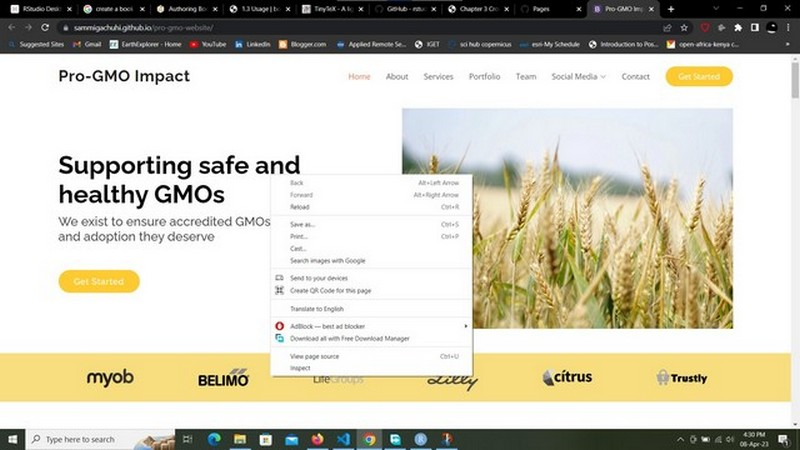
\includegraphics{../images/inspect.jpg}

Scroll over to the \textbf{Element} tab and you will have something that looks like this:

\begin{Shaded}
\begin{Highlighting}[]
\NormalTok{knitr}\SpecialCharTok{::}\FunctionTok{include\_graphics}\NormalTok{(}\FunctionTok{rep}\NormalTok{(}\StringTok{"D:/gachuhi/my{-}Leaflet/images/elements.jpg"}\NormalTok{))}
\end{Highlighting}
\end{Shaded}

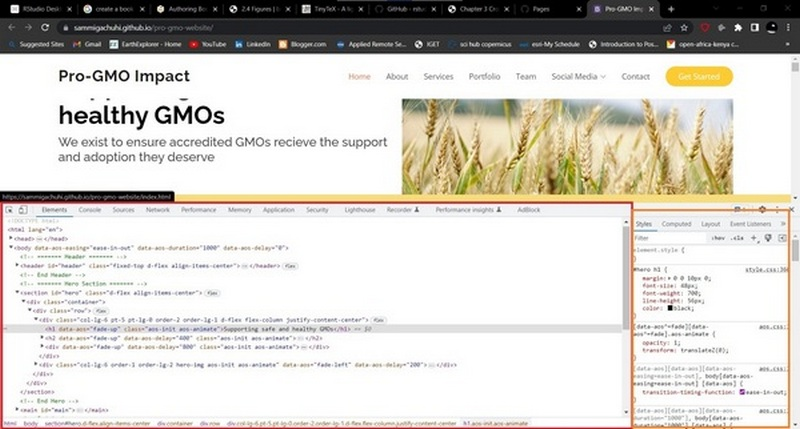
\includegraphics{../images/elements.jpg}

The part encircled in red is the \texttt{html} that makes up the webpage for the \href{https://sammigachuhi.github.io/pro-gmo-website/}{ProGMO website} in this case.

So, I am a GIS specialist, I want to learn how to make a HTML website so as to use Leaflet and its functionalities. Whereas this document does not provide an indepth view of all the ins and outs of a HTML document, HTML websites are made up of elements known as \texttt{tags}. Tags, normally indicated by angle brackets (\texttt{\textless{}\textgreater{}}) are what introduce any form of content into a webpage, be it a paragraph \texttt{(\textless{}p\textgreater{})}, an image \texttt{(\textless{}img\textgreater{})}, video \texttt{(\textless{}video\textgreater{})} and even an entire section (\texttt{\textless{}div\textgreater{}}, \texttt{\textless{}section\textgreater{}}, \texttt{\textless{}article\textgreater{}}). With this basic introduction, let's create a basic HTML page.

To create a HTML element along with many other programming files, such as \texttt{.js} and \texttt{.css} which we shall see later, we use a text editor. A good example of a text editor is VS code or Pycharm. Check their websites on their installation methods for your personal computer. For creating HTML and working with \texttt{.js} documents later, we shall use VS Code unless otherwise stated.

Here is a basic HTML webpage.

\begin{verbatim}
<!DOCTYPE html>
<html lang="en">
    <head>
        <title>A basic html webpage</title>
        <meta charset="utf-8">
        <link rel="stylesheet" href="style.css">
    </head>
    <body>
        <div id="division-1">
            <p>Hello, World!</p>
        </div>
        <script src="main.js">

        </script>

    </body>
</html>
\end{verbatim}

Let's go through each of the above tags one by one.

\begin{enumerate}
\def\labelenumi{\arabic{enumi}.}
\item
  \texttt{\textless{}!DOCTYPE\ html\textgreater{}} - It is an ``information'' to the browser about what document type to expect.
\item
  \texttt{\textless{}html\ lang="en"\textgreater{}} - It is the container for all other HTML elements (except for the \texttt{\textless{}!DOCTYPE\textgreater{}} tag). The \texttt{lang} attribute is used to assist web engines know which language the website uses.
\item
  \texttt{\textless{}head\textgreater{}} - It is not displayed on the webpage as other tags, but contains the metadata of the webpage.
\item
  \texttt{\textless{}title\textgreater{}} - Can you guess? You had it right. Defines the title of the document. In our case, if you open the webpage assuming you created it in VS Code, the webpage shall be titled \emph{A basic html webpage} at the tab of your web-browser.
\item
  \texttt{\textless{}meta\ charset="utf-8"\textgreater{}} - This is part of the metadata hosted by the \texttt{\textless{}head\textgreater{}} tag. We had mentioned earlier that the \texttt{\textless{}head\textgreater{}} contains the metadata of the webpage. Now here we would like to add that the \texttt{\textless{}meta\textgreater{}} tag found \emph{within} the \texttt{\textless{}head\textgreater{}} is what \emph{defines} the metadata. You can think of it as \textbf{README} text file that comes with any software you download. The \texttt{\textless{}meta\textgreater{}} tag in our case defines the encoding of our HTML5 document with the attribute \texttt{charset="utf-8"}. Don't think about this too much. HTML5 documents have \texttt{utf-8} as their encoding. You can try to look up what encoding is but it's not useful for this tutorial!
\item
  \texttt{\textless{}link\textgreater{}} - Defines the relationship between a document and an external resource. It has various attributes but \texttt{rel} and \texttt{href} have been used. The former specifies the relationship between the current document and the linked document/resource. The \texttt{rel} here references the \texttt{styles.css} file as the style sheet for our HTML. That is, the styles for our HTML are found in the \texttt{styles.css} file. \texttt{href} on the other hand points the HTML document to the path of the stylesheet --the \texttt{styles.css} file.
\item
  \texttt{\textless{}body\textgreater{}} - This is the crux of your webpage. If nothing is within the \texttt{\textless{}body\textgreater{}} tags, your webpage will be as empty as a blank sheet of paper. This tag is the home for all the other contents of the webpage such as headings, paragraphs, images, tables etc.
\item
  \texttt{\textless{}div\textgreater{}} - This is a special element that lets you group similar sets of content together on a web page. You can use it as a generic container for associating similar content. In the above HTML script, we have included an \texttt{\textless{}id\textgreater{}} attribute that is in other words, a unique identifier for this section of the webpage. \texttt{\textless{}id\textgreater{}s} are useful if you want to customize the appearance of a certain part of the webpage. \texttt{\textless{}class\textgreater{}}es behave in a similar way, but the difference between \texttt{\textless{}id\textgreater{}} and \texttt{\textless{}class\textgreater{}} is that \texttt{\textless{}id\textgreater{}} has to be unique, while \texttt{\textless{}class\textgreater{}}es can be used more than once.
\end{enumerate}

9.\texttt{\textless{}script\textgreater{}} - It is used to embed executable code or data. In most cases it refers to JavaScript, which enhances interactivity.

If you may have noticed above, most HTML tags end with \texttt{\textless{}/name-of-tag\textgreater{}}. With a few exceptions such as \texttt{\textless{}img\textgreater{}}, almost all HTML tags end this way.

\hypertarget{javascript}{%
\section{JavaScript}\label{javascript}}

JavaScript, shortened to \texttt{.js} is the language of the web. It introduces interactivity to HTML files. Without it our HTML files would just remain static. Have you ever clicked a link or a shiny button on a website and some visual or menu popped up? JavaScript was the engine behind all that. Think of \texttt{.js} as the life of the party while HTML is just the setting. Without \texttt{.js}, creating webmaps would not be possible since adding JavaScript code to a HTML file using \texttt{\textless{}script\textgreater{}} is what makes the map appear on any website!

\hypertarget{css-files}{%
\section{CSS files}\label{css-files}}

CSS stands for \emph{Cascading Style Sheet}. The CSS defines how your HTML is to appear, such as color and size of text, background color of the HTML as well as the structure of your HTML page.

CSS is quite a huge field despite appearing simple to the novice's eye. However, the html elements of a webpage are accompanied by a curly bracket containing the specified properties and values. The CSS terms `Properties' and `Values' are described below.

\begin{itemize}
\item
  Properties: These are human-readable identifiers that indicate which stylistic features you want to modify. For example, font-size, width, background-color.
\item
  Values: Each property is assigned a value. This value indicates how to style the property.
\end{itemize}

Using the example of our ProGMO website, this is how we would specify the font and color of the \texttt{\textless{}body\textgreater{}} element of our webpage. In some cases, the property values in CSS elements can be more than one, as in \texttt{font-family} below.

\begin{verbatim}
body {
  font-family: "Open Sans", sans-serif;
  color: #444444;
}
\end{verbatim}

The \texttt{body} in the CSS file is known as the selector. Selectors in CSS are what tags are to HTML files. However, selectors can be more specific, such as specifying the exact \texttt{\textless{}div\textgreater{}} that should be displayed in a particular way. Using our HTML file example, if there were other \texttt{\textless{}div\textgreater{}}s apart from the \texttt{\textless{}div\ id="division-1"\textgreater{}} above, we would specify the one with ID \texttt{division-1} in a CSS document like so:

\begin{verbatim}
#division-1 {
  font-family: "Open Sans", sans-serif;
  color: #343a40;
}
\end{verbatim}

We specify all specific IDs in a HTML file with a prefix of \texttt{\#}. Suppose there was a \texttt{\textless{}div\ id="division-2"\textgreater{}} somewhere in the HTML. We would similarly define some properties specific to it in the manner below:

\begin{verbatim}
#division-2 {
  font-family: helvetica;
  color: #000000;
}
\end{verbatim}

For \texttt{\textless{}classes\textgreater{}} and they can be several, we select each particular class using the convention:

\begin{verbatim}
.class_name {
property: value
prperty2: value2}
\end{verbatim}

You can view the style of a particular HTML element using the styles tab found in \textbf{Element} tab of the inspect console. To get to the \textbf{Inspect} tab of your browser, right click the webpage and select \textbf{Inspect} from the list of options provided.

\begin{Shaded}
\begin{Highlighting}[]
\NormalTok{knitr}\SpecialCharTok{::}\FunctionTok{include\_graphics}\NormalTok{(}\FunctionTok{rep}\NormalTok{(}\StringTok{"D:/gachuhi/my{-}Leaflet/images/elements2.jpg"}\NormalTok{))}
\end{Highlighting}
\end{Shaded}

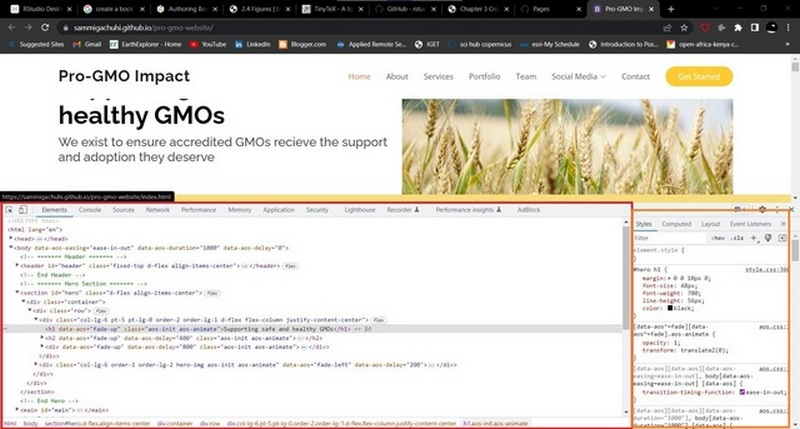
\includegraphics{../images/elements2.jpg}

The \href{https://developer.mozilla.org/en-US/docs/Learn/CSS/First_steps/How_CSS_is_structured}{MDN website} provides a lot of information on HTML and CSS.

\hypertarget{summary}{%
\section{Summary}\label{summary}}

This chapter was an introduction to Hyper Text Markup Language (HTML), JavaScript and Cascading Style Sheets (CSS) languages. You learnt the following:

\begin{itemize}
\item
  You can work with Leaflet in either a HTML or JavaScript file. In HTML,
  the JavaScript code must appear under the \texttt{\textless{}script\textgreater{}} tag.
\item
  HTML files are made up of elements called tags. Tags are features that introduce any form of content into a webpage.
\item
  JavaScript is the main language of the web. It is the language responsible for the interactivity in most websites.
\item
  CSS stands for Cascading Style Sheet (CSS). CSS defines how your HTML is to appear, such as color and size of text, background color and even the structure of your HTML page.
\end{itemize}

\hypertarget{first-leaflet-map}{%
\chapter{First Leaflet Map}\label{first-leaflet-map}}

\hypertarget{setting-the-superstructure}{%
\section{Setting the superstructure}\label{setting-the-superstructure}}

We had earlier mentioned that Javascript is the life of the party when it comes to webpages. In other words, it moves your web pages from a static sate to being interactive. You can think of it like the energy drink that makes an exhausted athlete want to do one more run.

Creating a Leaflet map is not like creating any other HTML web page. You have to set up the Leaflet essentials in your HTML page first. To begin with, create a new HTML document called \texttt{map.html}. This will be the HTML document that will act as the structure which will house our webpage to be created using JavaScript. Using VS Code, create \texttt{map.html} and paste, or preferably, type the following code.

\begin{verbatim}
<!DOCTYPE html>
<html lang="en">
    <head>
        <title>Leaflet Maps</title>
        <meta charset="utf-8">
        <link rel="stylesheet" href="styles.css">
        <link rel="stylesheet" href="https://unpkg.com/leaflet@1.9.3/dist/leaflet.css"
     integrity="sha256-kLaT2GOSpHechhsozzB+flnD+zUyjE2LlfWPgU04xyI="
     crossorigin=""/>
        <script src="https://unpkg.com/leaflet@1.9.3/dist/leaflet.js"
        integrity="sha256-WBkoXOwTeyKclOHuWtc+i2uENFpDZ9YPdf5Hf+D7ewM="
        crossorigin=""></script>
    </head>
    <body>
        <div id="myMap">
            <script src="main.js">
            </script> 
        </div>  
        
    </body>
</html>
\end{verbatim}

You may be wondering why we have two \texttt{\textless{}link\textgreater{}} and \texttt{\textless{}script\textgreater{}} tags. When a browser reads a HTML script, it reads it from top to bottom. In our html script, the browser will apply the styles defined in \texttt{styles.css} to the HTML elements. To make matters clearer, the following script is what is contained in the \texttt{styles.css}:

\begin{verbatim}
#myMap { 
    height: 600px; 
}
\end{verbatim}

The CSS values, those within the curly brackets, will be responsible for making our map canvas have a height of 600px on the browser.

Now to the two \texttt{\textless{}script\textgreater{}} tags. One refers to the online JavaScript library. The \texttt{src} attribute is in fact linking to a webpage as you can see from the protocol-- \texttt{https://...}. The second, housed under the \texttt{\textless{}div\textgreater{}} tag, references our local JavaScript file which shall contain all the code to transform our HTML page to a webmap ninja --lines, polygons and other cool stuff.

\hypertarget{beautifying-the-house}{%
\section{Beautifying the house}\label{beautifying-the-house}}

Think of the HTML document as the superstructure, like a huge multistorey building just finished. Though the structure has the best architectural design, it just looks all grey with no life unless we call some exterior designers to add some color. That's what \texttt{main.js} file, pointed to by the \texttt{\textless{}script\textgreater{}} tag in the HTML document will precisely do. Through the help of JavaScript, our static HTML file will turn into an interactive map.

Open your VS Code, and assuming you had already created \texttt{main.js} already, (if not, create one now), insert the following code into the \texttt{.js} file.

\begin{verbatim}
var map = L.map('myMap').setView([-0.0884105,34.7299038], 13);
\end{verbatim}

Take a pause.

Breath in, breath out.

You are just about to learn something very important here. In fact, it is the crux of what makes Leaflet work. Your understanding of leaflet hinges on the small code above.

The \texttt{L.map()} class we just used is what initializes the Leaflet map. Everything within the \texttt{\textless{}div\textgreater{}} is displayed thanks to this class function. It is referred to as a factory function because it uses the method \texttt{map} to return an object.

The \texttt{setView} method \emph{sets the view of the map (geographical center and zoom) with the given animation options}. It's properties are Latitude-Longitude, zoom number and other options. All Leaflet methods and functions are explained in the {[}\href{https://leafletjs.com/reference.html}{Leaflet reference}. Not that we have inserted at Latitude, Longitude and zoom level respectively within the \texttt{setView} method.

Try loading your \texttt{map.html}. All you see is a grey canvas with zoom options. This is because we haven't added a tilelayer yet. A \href{https://pro.arcgis.com/en/pro-app/latest/help/data/services/use-tiled-web-layers.htm}{tileLayer} is a set of web-accessible tiles that reside on a server. A tile consists individual images or vector files from a server which are collectively joined together to form a webmap. If you've zoomed into a webmap, say Google Maps and noticed boxes appearing as you zoomed in or out, those are \emph{tiles}.

Let's load an example of a common tile layer--the Open StreetMap--into Leaflet.

\begin{verbatim}
L.tileLayer('https://tile.openstreetmap.org/{z}/{x}/{y}.png', {
    maxZoom: 19,
    attribution: '&copy; <a href="http://www.openstreetmap.org/copyright">OpenStreetMap</a>'
}).addTo(map);
\end{verbatim}

Reload your HTML page again. You should see an web map like the one below.

\begin{Shaded}
\begin{Highlighting}[]
\NormalTok{knitr}\SpecialCharTok{::}\FunctionTok{include\_graphics}\NormalTok{(}\FunctionTok{rep}\NormalTok{(}\StringTok{"D:/gachuhi/my{-}leaflet/images/kisumu{-}leaflet.jpg"}\NormalTok{))}
\end{Highlighting}
\end{Shaded}

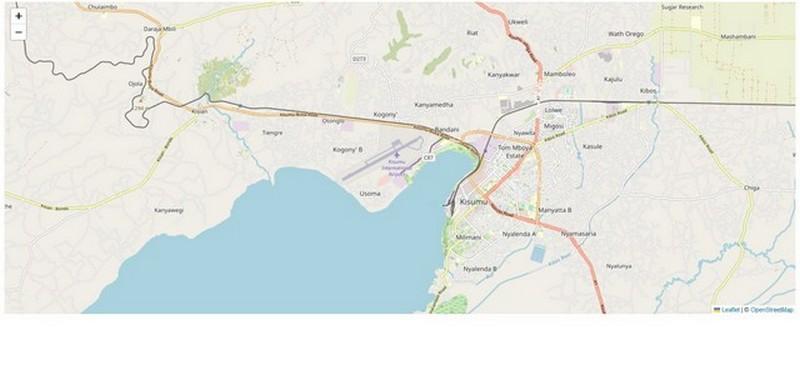
\includegraphics{../images/kisumu-leaflet.jpg}

What \texttt{L.tileLayer} has done is retrieve the web tiles from the Uniform Resource Locator (url) source provided, and within the dictionary that follows the url, zoom level (\texttt{maxZoom}) and map attribution (\texttt{attribution}) have been provided. When working with Leaflet, the dictionary, indicated by the curly braces \texttt{\{\}} houses most of the additional class options other than the key one(s). In this case we used the additional options of \texttt{maxZoom} and \texttt{attribution}. Finally, the method \texttt{addTo} adds the layer to the given map or layer group. Here, our webtile is added to the \texttt{var\ map} which only contains the \texttt{setView} properties.

A very influential person said Kisumu located in Kenya is a town with great potential. How about dispalying it to the whole world to realise it!

\hypertarget{summary-1}{%
\section{Summary}\label{summary-1}}

In this chapter, we created our first Leaflet map. Here are a couple of things that you have learnt at the first step of this web mapping journey.

\begin{itemize}
\item
  Browsers read code scripts from top to bottom, much like skimming down a page.
\item
  The styles defined in the CSS style sheet, the \texttt{styles.css} in this case, will apply to the HTML elements in the \texttt{map.html} file.
\item
  We use the \texttt{src} attribute to link a different file other than HTML, such as a JavaScript file, to your HTML file. For example, the online script \texttt{leaflet.js} is connected to the HTML file through the \texttt{src} attribute of the \texttt{\textless{}script\textgreater{}} to enable the HTML file execute Leaflet functionalities such as web map creation, rendering and controls.
\item
  If HTML is the magnificent building, JavaScript acts like a good exterior designer.
\item
  The \texttt{L.map()} class is what initializes the Leaflet map.
\end{itemize}

\hypertarget{add-ons}{%
\chapter{Add ons}\label{add-ons}}

\hypertarget{not-just-a-plain-map}{%
\section{Not just a plain map}\label{not-just-a-plain-map}}

Like in the ultimate finale of a series where the episode begins with the statement- ``Previously on\ldots{}'', this chapter shall be a continuation of \protect\hyperlink{first-leaflet-map}{Chapter 2}.

So we have a plain looking webmap like the one shown below.

\begin{Shaded}
\begin{Highlighting}[]
\NormalTok{knitr}\SpecialCharTok{::}\FunctionTok{include\_graphics}\NormalTok{(}\FunctionTok{rep}\NormalTok{(}\StringTok{"D:/gachuhi/my{-}leaflet/images/kisumu{-}leaflet.jpg"}\NormalTok{))}
\end{Highlighting}
\end{Shaded}

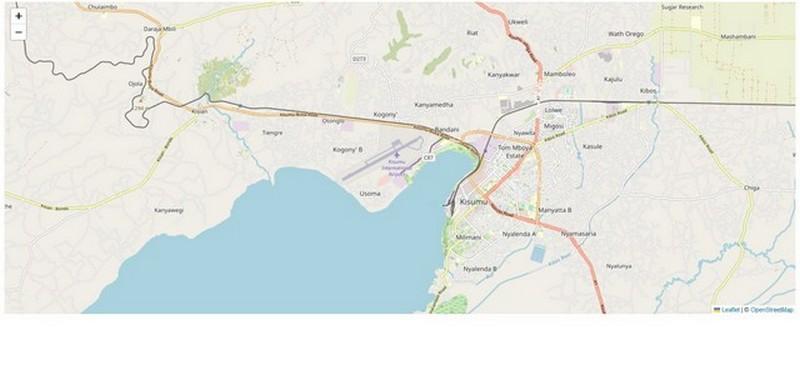
\includegraphics{../images/kisumu-leaflet.jpg}

However, despite being a cool looking webmap, it offers no other additional information to the user. In order to pass some information, such as showing the location of Kisumu and \emph{inter alia}, markers are one way of displaying such content. As a side note, there are other basemap layer servers compatible with Leaflet available \href{https://leaflet-extras.github.io/leaflet-providers/preview/}{here}.

\hypertarget{a-marker}{%
\section{A marker}\label{a-marker}}

Many people could possibly hardly know where Kisumu, is, so lets indicate its location with a simple pin marker. To be more specific, let's pinpoint Kisumu International Airport.

\begin{verbatim}
// Location of Kisumu International Airport
var marker = L.marker([-0.0819301, 34.7260167]).addTo(map);
\end{verbatim}

\begin{Shaded}
\begin{Highlighting}[]
\NormalTok{knitr}\SpecialCharTok{::}\FunctionTok{include\_graphics}\NormalTok{(}\FunctionTok{rep}\NormalTok{(}\StringTok{"D:/gachuhi/my{-}leaflet/images/kisumu{-}international{-}airport.jpg"}\NormalTok{))}
\end{Highlighting}
\end{Shaded}

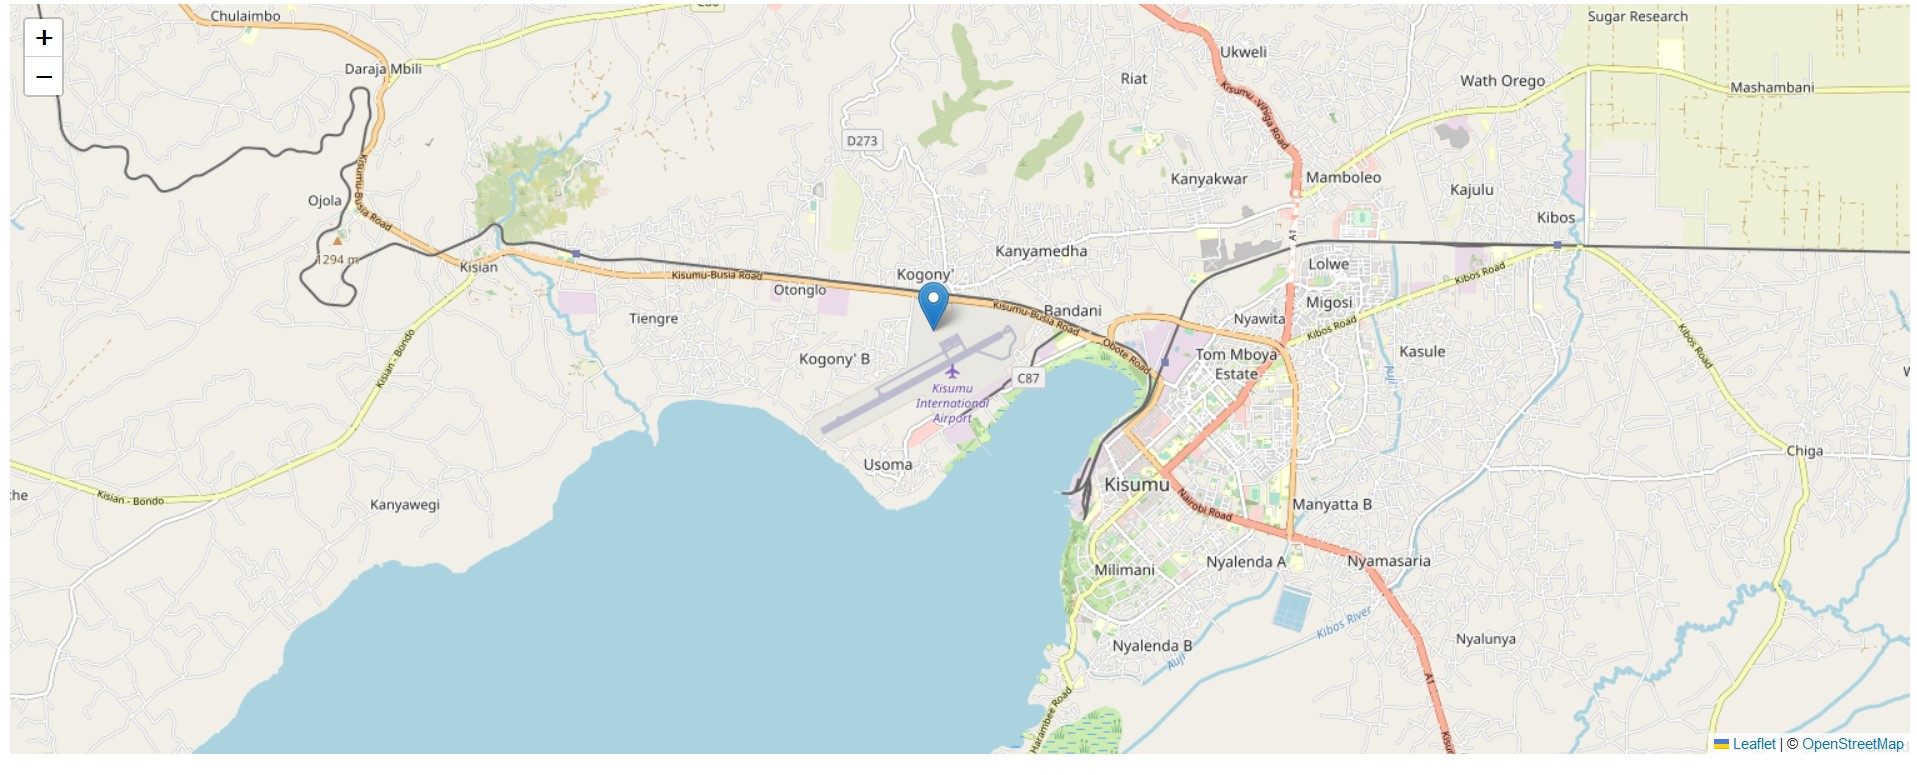
\includegraphics{../images/kisumu-international-airport.jpg}

As a simple exercise, can you try creating a marker for your home location using the \texttt{setView} method you have learned about so far?

Alright, we have a marker. But what's so special about it apart from it being a lone pin in the middle of somewhere? Let's try to make this marker have some information, otherwise called attributes in GIS. Let's say the attributes we want to add are the name of the airport and other auxillary data.

\hypertarget{a-marker-with-a-popup}{%
\section{A marker with a popup}\label{a-marker-with-a-popup}}

To create popups, Leaflet provides the \texttt{bindPopup} method. You just \emph{chain} it to the variable, more like how you would add an extension to a browser to perform new functions but now in this case, these extra functions are added to the variable. In the below code, \texttt{bindPopup} is chained to the \texttt{marker} variable using a dot \texttt{.}.

\begin{verbatim}
// Create popup of Kisumu international Airport
marker.bindPopup("Kisumu International Airport.").openPopup();
\end{verbatim}

\begin{Shaded}
\begin{Highlighting}[]
\NormalTok{knitr}\SpecialCharTok{::}\FunctionTok{include\_graphics}\NormalTok{(}\FunctionTok{rep}\NormalTok{(}\StringTok{"D:/gachuhi/my{-}leaflet/images/kisumu{-}airport{-}popup.jpg"}\NormalTok{))}
\end{Highlighting}
\end{Shaded}

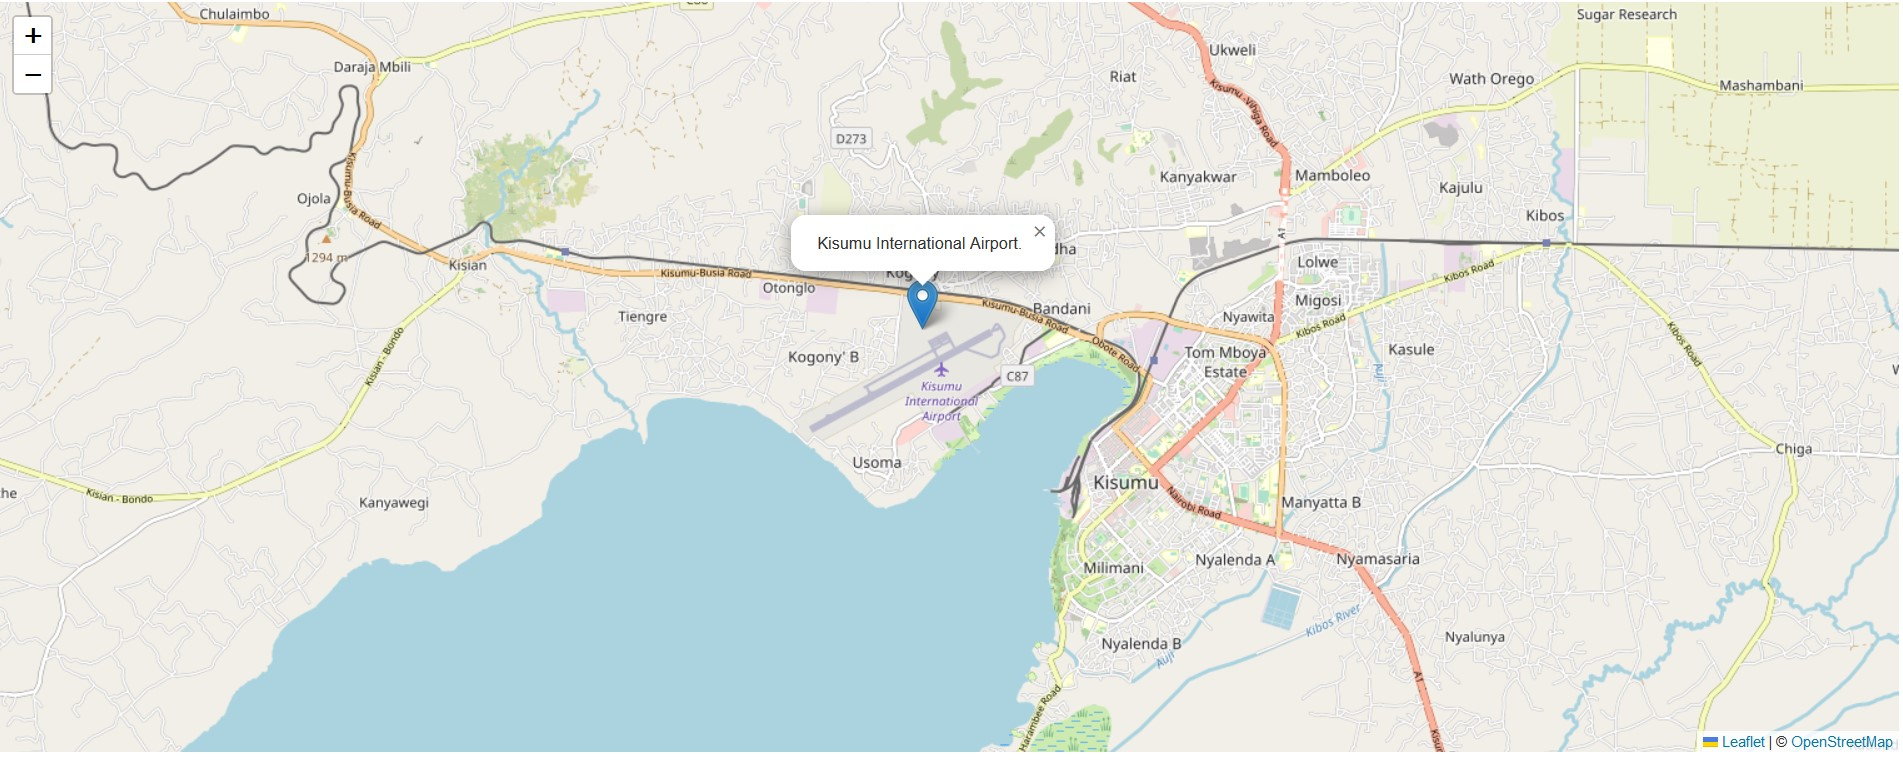
\includegraphics{../images/kisumu-airport-popup.jpg}

What has just happened is that \texttt{bindPopup} binds the popup content-- ``Kisumu International Airport'' to the marker. In the below code, we have added another method, \texttt{openPopup} which \emph{open} the popup at that specified latitude longitude. If you remove, or comment \texttt{//} out the \texttt{popUp} method, you will have to click the marker to see the popup content. Try it out.

Markers can also work with HTML elements, such as when you want to display additional metadata, say the owner of the place, size of land et cetera. In the below case, we have added the lat-lon coordinates of Kisumu airport location. It is highly advised not to include lengthy information in an HTML marker element.

\begin{verbatim}
// With html content
marker.bindPopup("<br>Name: Kisumu International Airport</br><br>Latitude: -0.0819301</br><br>Longitude: 34.7260167</br>").openPopup();
\end{verbatim}

\begin{Shaded}
\begin{Highlighting}[]
\NormalTok{knitr}\SpecialCharTok{::}\FunctionTok{include\_graphics}\NormalTok{(}\FunctionTok{rep}\NormalTok{(}\StringTok{"D:/gachuhi/my{-}leaflet/images/marker{-}html.jpg"}\NormalTok{))}
\end{Highlighting}
\end{Shaded}

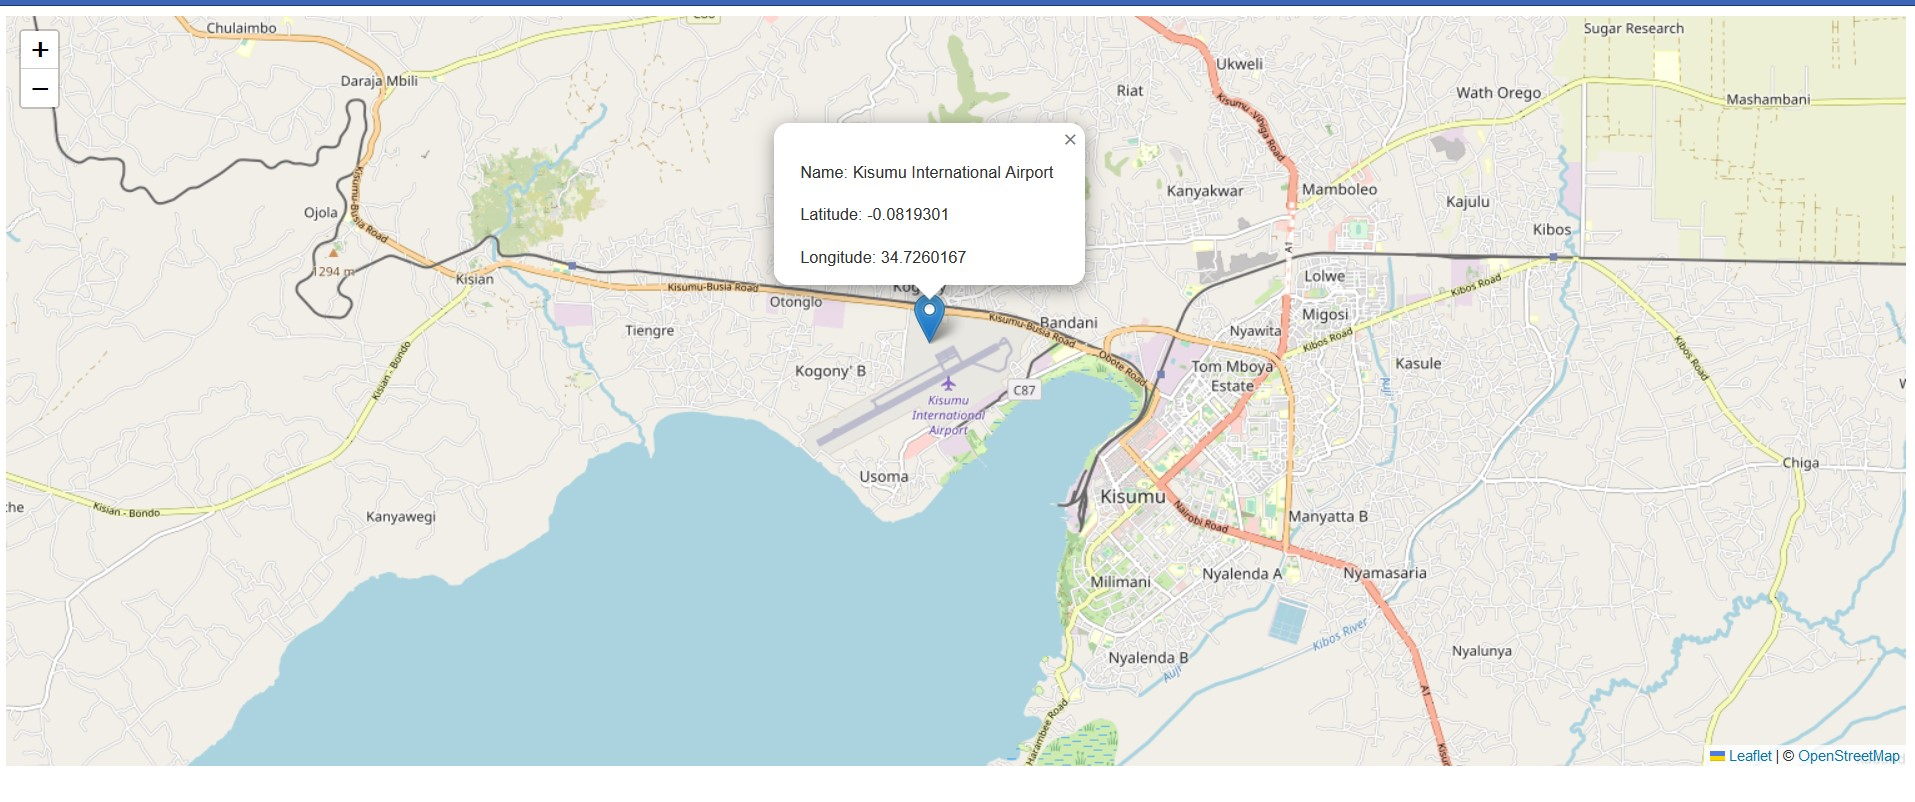
\includegraphics{../images/marker-html.jpg}

\hypertarget{different-markers-and-popups}{%
\section{Different markers and popups}\label{different-markers-and-popups}}

So far you have seen pin markers, but there are also other kinds of markers, such as circles and rectangles. Unlike the pin markers we have been experimenting with, these other markers require additional options, such as radius value for circle and lat-long coordinates for rectangles. Let's have a go with each type.

Starting with a circle, let's start by drawing a radius around the location of Kisumu Museum.

\begin{verbatim}
// Circle over Kisumu Museum
var circle = L.circle([-0.107637, 34.7435975]).setRadius(2000).addTo(map);
\end{verbatim}

\begin{Shaded}
\begin{Highlighting}[]
\NormalTok{knitr}\SpecialCharTok{::}\FunctionTok{include\_graphics}\NormalTok{(}\FunctionTok{rep}\NormalTok{(}\StringTok{"D:/gachuhi/my{-}leaflet/images/kisumu{-}museum{-}circle.jpg"}\NormalTok{))}
\end{Highlighting}
\end{Shaded}

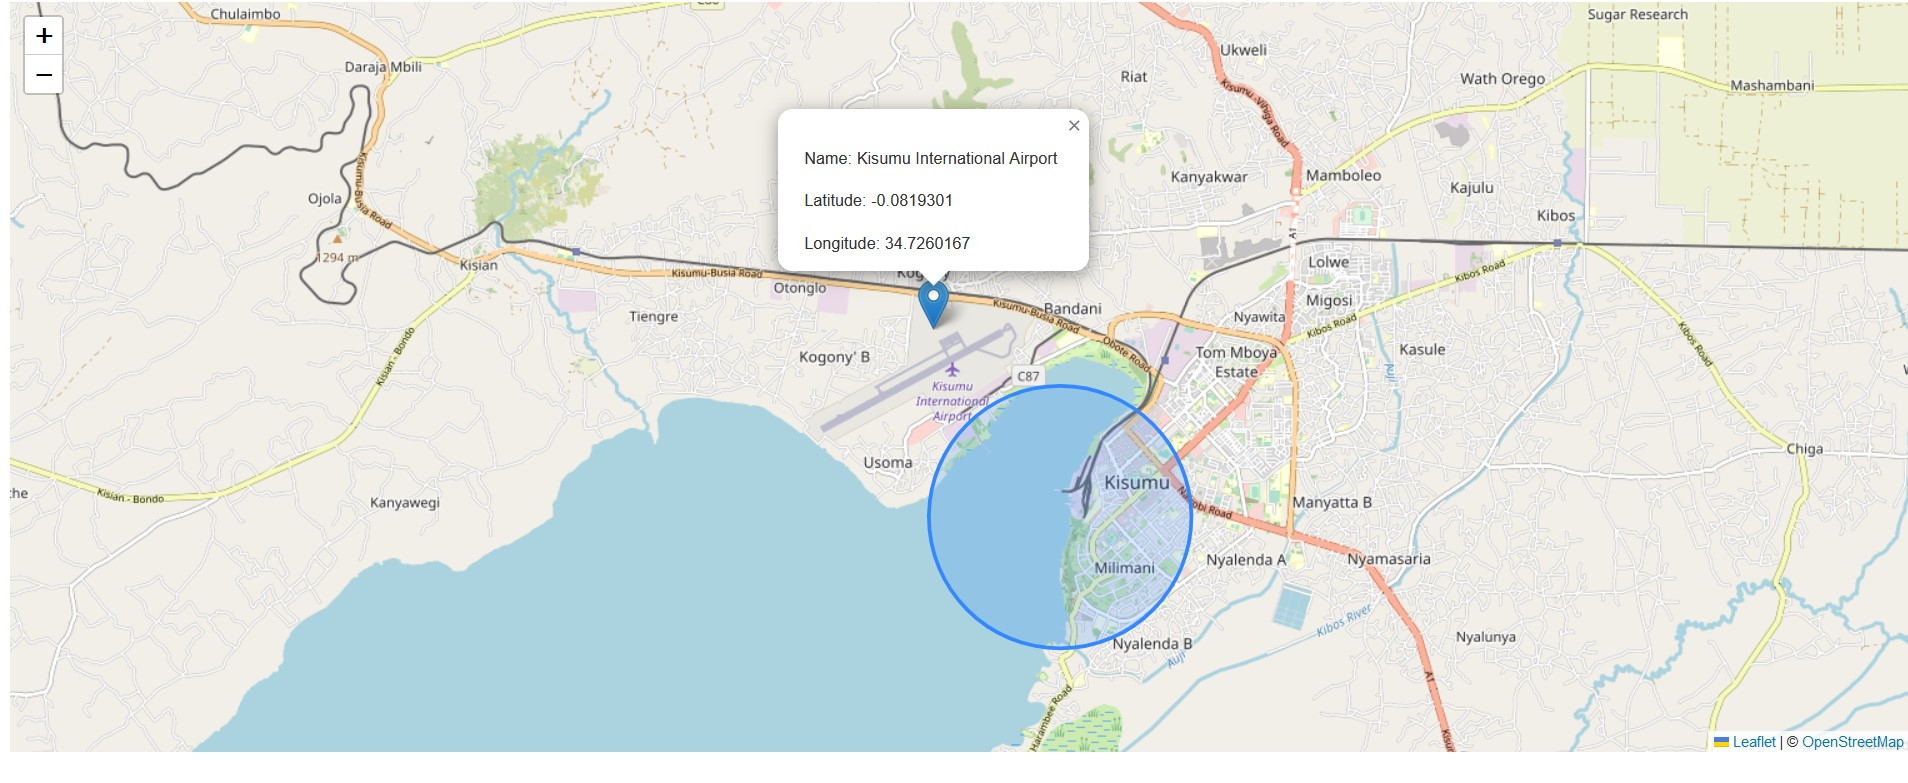
\includegraphics{../images/kisumu-museum-circle.jpg}

The below code will also create a slightly similar circle marker, the only difference is that in the preceding one we didn't insert \texttt{\{options\}} and we set radius using the \texttt{setRadius} method. In the second one below, we have been very specific in what we want --our specifications going into the curly brackets \{\} before eventually adding the circle marker to our map. Brackets in JavaScript indicate you are dealing with a \href{https://flexiple.com/javascript/javascript-dictionary/}{dictionary}. A dictionary in JavaScript and even in Python is used to denote key-value pairs.

\begin{verbatim}
var circle = L.circle([-0.107637, 34.7435975], {
    color: 'blue',
    fillColor: 'blue',
    fillOpacity: .5,
    radius: 2000
}).addTo(map);
\end{verbatim}

As we had mentioned earlier, other marker elements such as circles and rectangles can have popups attached to them. Ready for something cool? We will attach a popup into our circle. Not just any other ordinary hard coded popup but one which relies on other Leaflet JavaScript methods to generate an output. In our case, we want a pop up that shows the radius of our circle, without us typing it out into the code.

\begin{verbatim}
// Circle marker pop up for Kisumu Museum
var getRadius = circle.getRadius();
circle.bindPopup("Radius is: " + getRadius.toString() + " metres");
\end{verbatim}

In our above code, \texttt{getRadius} gets the radius of our circle marker. \texttt{bindPopup} as has already been explained before \emph{binds} the popup content to our circle marker. But there is a catch. The variable \texttt{getRadius} is used to print out the results, which is 2000 of course. However, \texttt{bindPopup} only understands strings so we convert our variable result to a string using \texttt{toString()}. We also added other strings to give the popup a wholesome result that is understandable to every Tom, Dick, Harry and Harriet.

\begin{Shaded}
\begin{Highlighting}[]
\NormalTok{knitr}\SpecialCharTok{::}\FunctionTok{include\_graphics}\NormalTok{(}\FunctionTok{rep}\NormalTok{(}\StringTok{"D:/gachuhi/my{-}leaflet/images/circle{-}radius.jpg"}\NormalTok{))}
\end{Highlighting}
\end{Shaded}

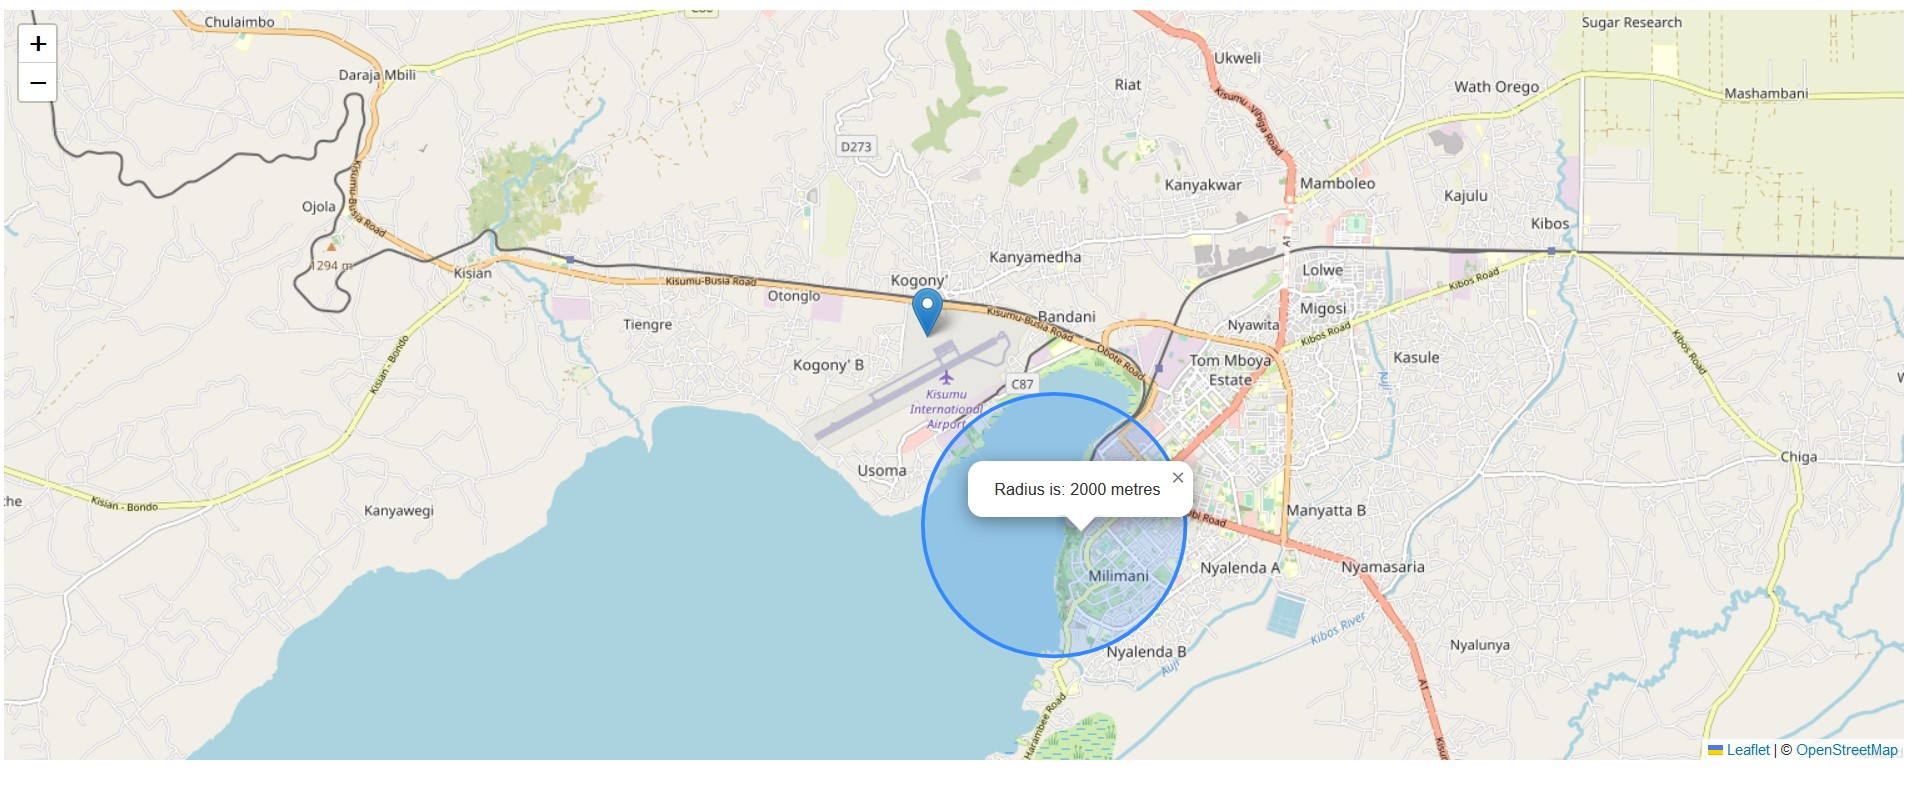
\includegraphics{../images/circle-radius.jpg}

Finally, let's try with a rectangle. Actually, Leaflet allows us to create polygons. Let's work with the polygon class to create a rectangle bounding a given location.

Copy the following coordinates.

\begin{verbatim}
// Draw rectangle around Kisumu Wildlife Impala Park
var impalaParkCoordinates = [
    [-0.1144753, 34.743418],
    [-0.115097, 34.745242],
    [-0.114238, 34.745071],
    [-0.114002, 34.746101],
    [-0.115054, 34.746787],
    [-0.115998, 34.745586],
    [-0.118444, 34.746208],
    [-0.121255, 34.744684]
]
\end{verbatim}

Now using the \texttt{L.polygon} class and a few optional parameters, let's showcase where the Kisumu Wildlife Impala Park is situated.

\begin{verbatim}
// Create a polygon using the above coordinates
var impalaParkPolygon = L.polygon(impalaParkCoordinates, {
    color: 'brown',
    fillOpacity: 0.4
}).addTo(map);
\end{verbatim}

Just like we did for the circle marker, we will make our popup content rely on another variable, in this case \texttt{getCenter} which gets the centroid coordinates of our polygon. We were looking for something cooler such as \texttt{getArea} in Leaflet, one that automatically prints out the area of a polygon in a popup. Unfortunately, we were unable to find it.

\begin{verbatim}
// Add popup to the polygon of Kisumu Impala Park
var getCenter = impalaParkPolygon.getCenter();
impalaParkPolygon.bindPopup("Centre is at Lat-Lon: " + getCenter.toString()).openPopup();
\end{verbatim}

If you find the circle marker too much of an obstraction to the rectangle marker, feel free to comment it out using \texttt{//}.

\begin{Shaded}
\begin{Highlighting}[]
\NormalTok{knitr}\SpecialCharTok{::}\FunctionTok{include\_graphics}\NormalTok{(}\FunctionTok{rep}\NormalTok{(}\StringTok{"D:/gachuhi/my{-}leaflet/images/polygon{-}marker.jpg"}\NormalTok{))}
\end{Highlighting}
\end{Shaded}

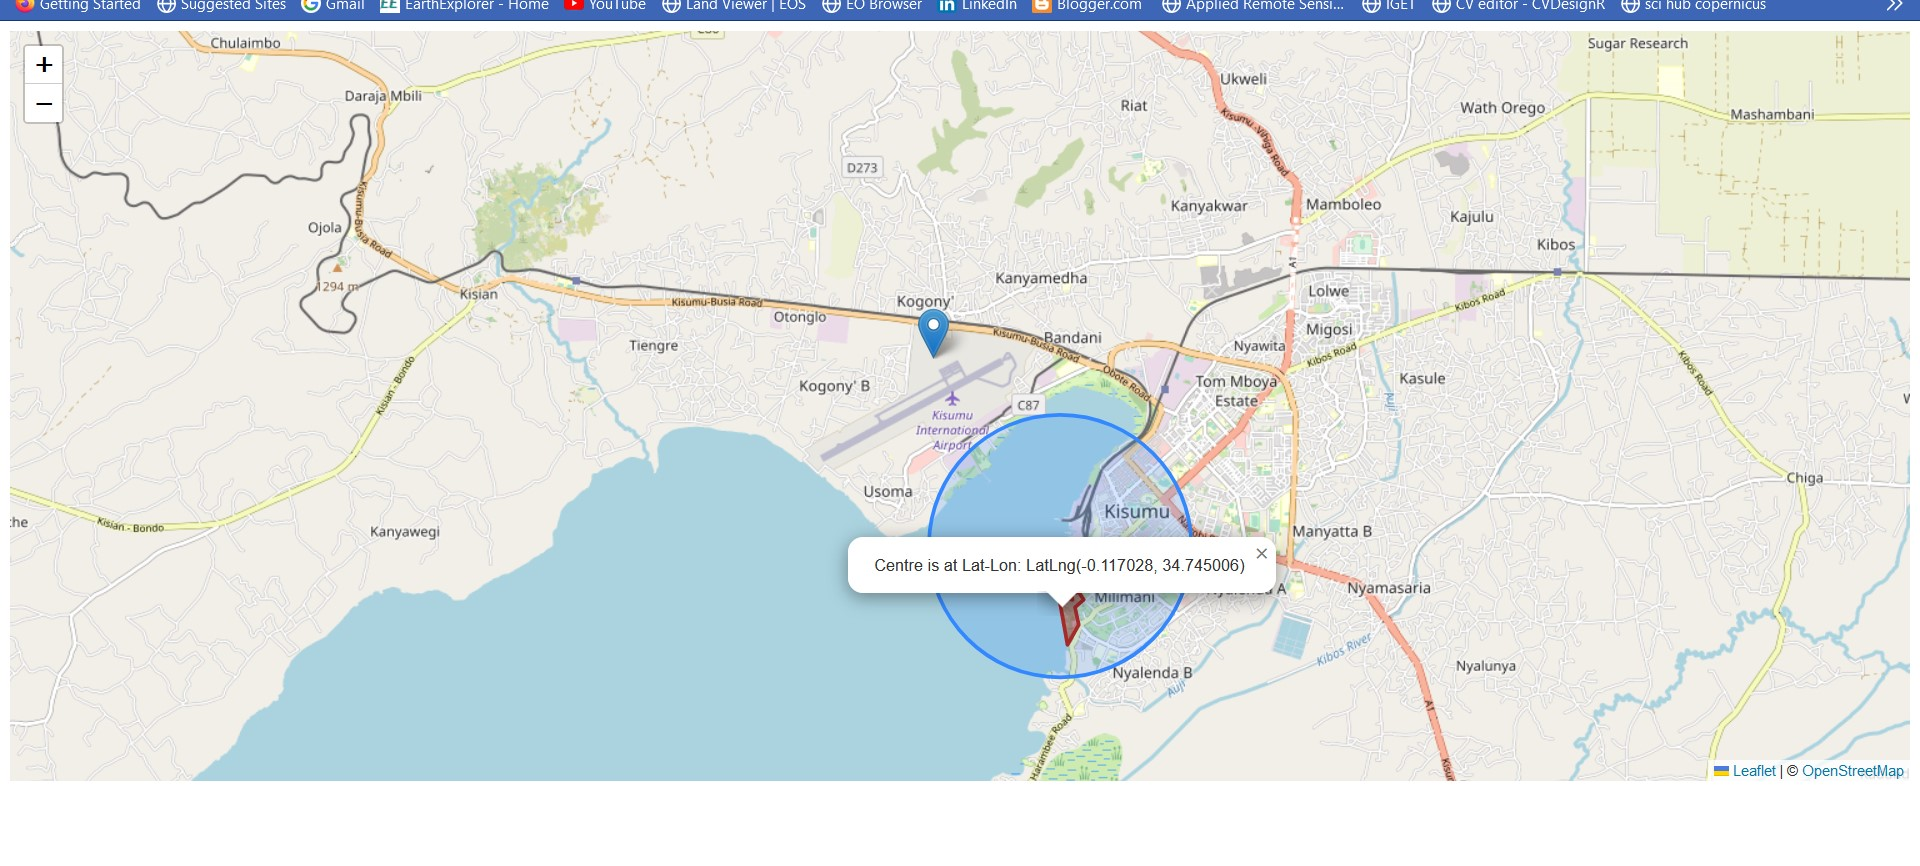
\includegraphics{../images/polygon-marker.jpg}

You can get the files used in this exercise \href{https://github.com/sammigachuhi/my-leaflet-project/tree/main/my-leaflet-code/chapter-3-markers}{here}.

\hypertarget{summary-2}{%
\section{Summary}\label{summary-2}}

This chapter took you further in enriching the content that can be displayed in a webmap. You have seen that a webmap can offer far more useful information than just mere markers and symbols on a web canvas. Popups are one way of displaying information, and they too can be customized further. Through the practicals in this chapter, you have learnt the following:

\begin{itemize}
\item
  To create popups in Leaflet, we use the \texttt{bindPopup} method.
\item
  \texttt{openPopup} automatically opens the popups once the Leaflet map is loaded. They only disappear once you close them.
\item
  Markers can also work with HTML elements.
\item
  Apart from location pins, markers can also be circles and rectangles.
\item
  There exist methods in Leaflet that can automatically parse out information in popups without requiring any hardcoding from the programmer. For example, we used \texttt{getRadius} to display the circle radius in the popup without necessarily typing it out in the \texttt{bindPopup} method.
\item
  You comment out JavaScript code with \texttt{//}!
\end{itemize}

\hypertarget{embedding-leaflet-map-to-an-external-website}{%
\chapter{Embedding leaflet map to an external website}\label{embedding-leaflet-map-to-an-external-website}}

\hypertarget{a-website-with-a-sense-of-direction}{%
\section{A website with a sense of direction}\label{a-website-with-a-sense-of-direction}}

Now, we have succeeded in making a stand alone leaflet map. However, we want to do something that will quickly upscale you from a novice to a pro. That is, embeding a Leaflet map into a website.

An example of what we want is shown below, which is a snapshot from the \href{https://data.humdata.org/dataset/cod-ab-ken}{HDX website}.

\begin{Shaded}
\begin{Highlighting}[]
\NormalTok{knitr}\SpecialCharTok{::}\FunctionTok{include\_graphics}\NormalTok{(}\FunctionTok{rep}\NormalTok{(}\StringTok{"D:/gachuhi/my{-}leaflet/images/webmap{-}in{-}web.jpg"}\NormalTok{))}
\end{Highlighting}
\end{Shaded}

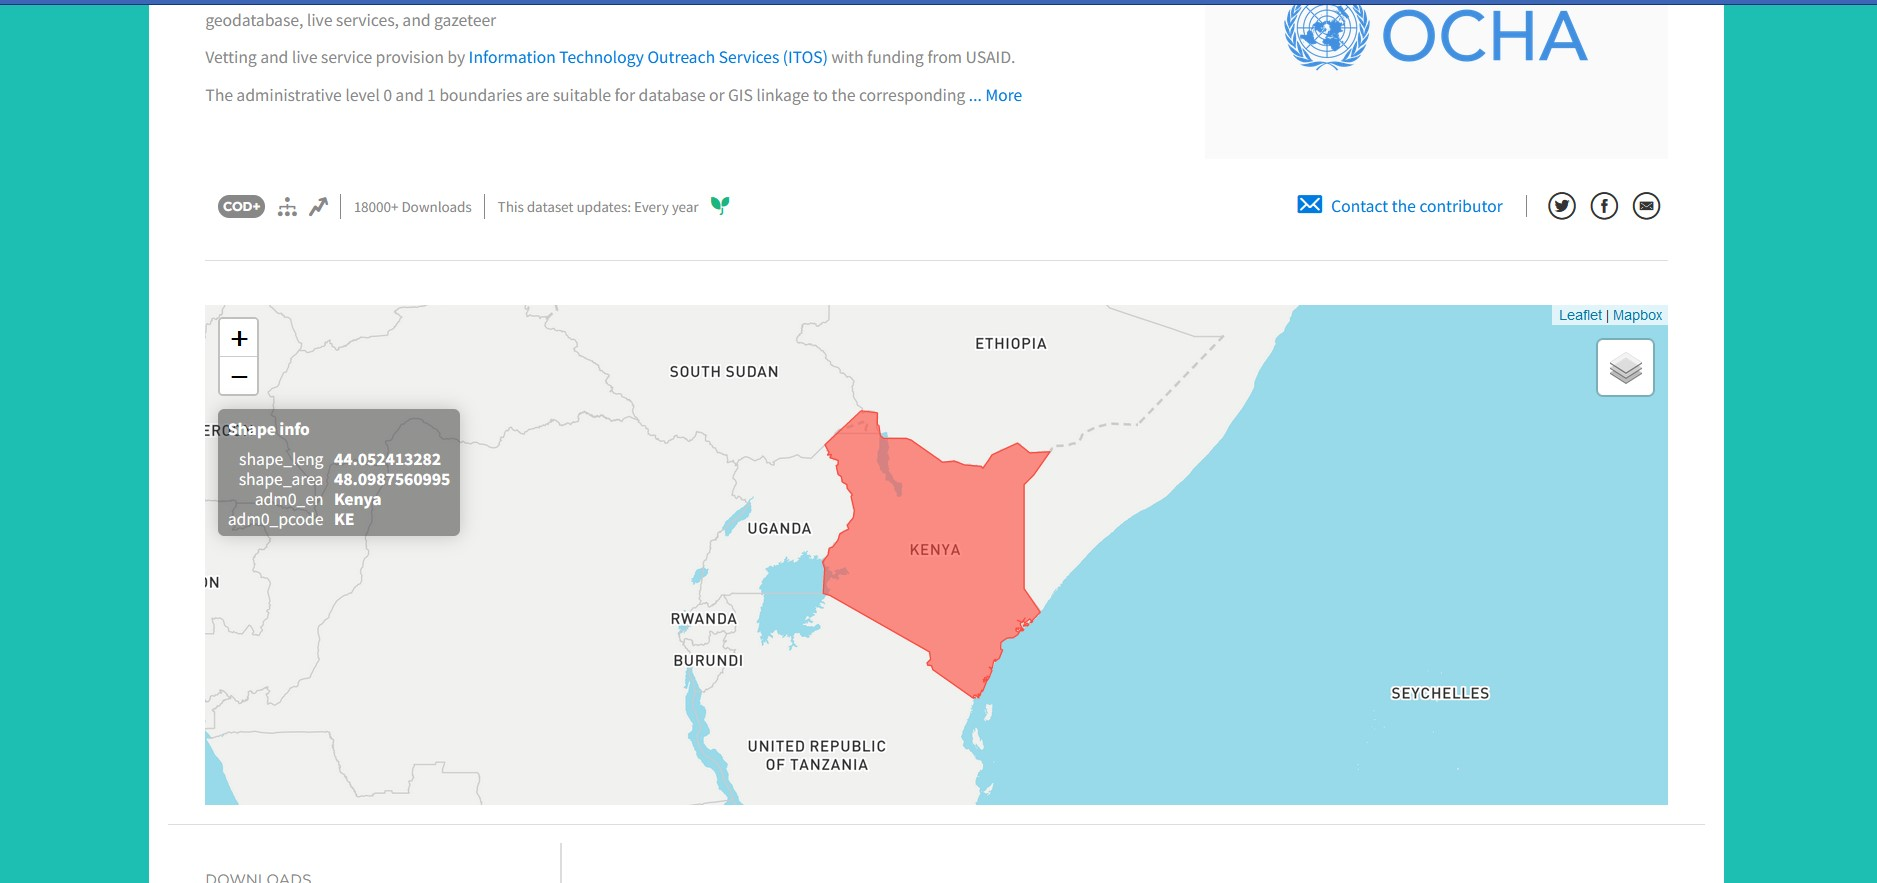
\includegraphics{../images/webmap-in-web.jpg}

For this exercise, we shall embed a leaflet map to a simple HTML webpage. This webpage doesn't look grand, but it serves the purpose of our exercise. Let's get on to it. Here are the \href{https://github.com/sammigachuhi/my-leaflet-project/tree/main/my-leaflet-code/chapter-4-embed-leaflet-website}{files}.

\hypertarget{the-html-webpage}{%
\section{The HTML webpage}\label{the-html-webpage}}

Create a HTML page with the following code.

\begin{verbatim}
<!DOCTYPE html>
<html lang="en">
    <head>
        <title>Pro-GMO Alliance</title>
        <meta charset="utf-8">
        <link rel="stylesheet" href="example-styles.css">
        <link rel="stylesheet" href="https://unpkg.com/leaflet@1.9.3/dist/leaflet.css"
        integrity="sha256-kLaT2GOSpHechhsozzB+flnD+zUyjE2LlfWPgU04xyI="
        crossorigin=""/>
        <script src="https://unpkg.com/leaflet@1.9.3/dist/leaflet.js"
        integrity="sha256-WBkoXOwTeyKclOHuWtc+i2uENFpDZ9YPdf5Hf+D7ewM="
        crossorigin=""></script>
    </head>
    <body>
    <div id="div-for-article">
        <article id="introduction">
            <h2>Introduction</h2>
            <q>Sed ut perspiciatis unde omnis iste natus error sit voluptatem accusantium 
            doloremque laudantium, totam rem aperiam, eaque ipsa quae ab illo inventore veritatis et 
            quasi architecto beatae vitae dicta sunt explicabo. Nemo enim ipsam voluptatem quia voluptas 
            sit aspernatur aut odit aut fugit, sed quia consequuntur magni dolores eos qui ratione 
            voluptatem sequi nesciunt. Neque porro quisquam est, qui dolorem ipsum quia dolor sit amet, 
            consectetur, adipisci velit, sed quia non numquam eius modi tempora incidunt ut labore et 
            dolore magnam aliquam quaerat voluptatem. Ut enim ad minima veniam, quis nostrum exercitationem 
            ullam corporis suscipit laboriosam, nisi ut aliquid ex ea commodi consequatur? Quis autem 
            vel eum iure reprehenderit qui in ea voluptate velit esse quam nihil molestiae consequatur, 
            vel illum qui dolorem eum fugiat quo voluptas nulla pariatur?</q>
        </article>
    </div>
    <div id="div-for-section">
        <section id="Products">
            <div class="row">
                <h2>Our Products</h2>
                <div class="column">
                  <img src="https://images.unsplash.com/photo-1632125941710-35a9d2fcc7ce?ixlib=rb-4.0.3&ixid=MnwxMjA3fDB8MHxwaG90by1wYWdlfHx8fGVufDB8fHx8&auto=format&fit=crop&w=1170&q=80" alt="Maize" style="width:100%">
                </div>
                <div class="column">
                    <img src="https://images.unsplash.com/photo-1595615636850-3292eb0a95b0?ixlib=rb-4.0.3&ixid=MnwxMjA3fDB8MHxwaG90by1wYWdlfHx8fGVufDB8fHx8&auto=format&fit=crop&w=1170&q=80" alt="Sunflower" style="width:100%">
                  </div>
                <div class="column">
                  <img src="https://images.unsplash.com/photo-1600333859399-228aa03f7dba?ixlib=rb-4.0.3&ixid=MnwxMjA3fDB8MHxwaG90by1wYWdlfHx8fGVufDB8fHx8&auto=format&fit=crop&w=1170&q=80" alt="Potato" style="width:100%">
                </div>
                <div class="column">
                  <img src="https://images.unsplash.com/photo-1630145398476-853543b02843?ixlib=rb-4.0.3&ixid=MnwxMjA3fDB8MHxwaG90by1wYWdlfHx8fGVufDB8fHx8&auto=format&fit=crop&w=1167&q=80" alt="Cotton" style="width:100%">
                </div>
              </div>
        </section>
    </div>
    <div>
        <br>
        <h2>Our Branches</h2>
        <br>
    </div>
      <div class="container">
        <div id="map">
          <script src="example-main.js"></script>
        </div>
        <div class="text">
          <h1>Address</h1>
          <p>
            P.O. Box 55044, Nakuru
        </p>
        </div>
      </div>
    </body>
</html>
\end{verbatim}

Since this is a geospatial book, we shall not go through every line of the HTML script above. It just a webpage containing some text, some pictures and a webmap. The webmap is the centre of our interest in this chapter. We at least do know how to create a Leaflet map, but how do we fit it inside a webpage?

Before we head there, let's insert the CSS file, which looks like this.

\begin{verbatim}
/* Three image containers (use 25% for four, and 50% for two, etc) */
.column {
    float: left;
    width: 33.33%;
    padding: 5px;
  }
  
  /* Clear floats after image containers */
  .row::after {
    content: "";
    clear: both;
    display: table;
  }


/* Styling the map */
  .container {
    display: flex;
    align-items: center;
    justify-content: center
  }

#map {
    height: 300px; 
    width: 90%
}

.text {
    font-size: 15px;
    padding-left: 20px;
}
\end{verbatim}

\hypertarget{a-simple-for-loop-for-webmap-display}{%
\section{\texorpdfstring{A simple \texttt{for} loop for webmap display}{A simple for loop for webmap display}}\label{a-simple-for-loop-for-webmap-display}}

Back to the Leaflet map of our dummy Pro-GMO Alliance webpage. How did we put the Leaflet in there? In just under a minute, parsing the JavaScript Leaflet file to the \texttt{\textless{}script\textgreater{}} tag and referencing it using the \texttt{src} attribute makes our webmap appear at its placed position in the HTML file. The JavaScript file we parsed to our HTML file is called \texttt{example-main.js}. It contains the following code:

\begin{verbatim}
var map = L.map('map').setView([-0.302765, 36.146147], 12);

L.tileLayer('https://tile.openstreetmap.org/{z}/{x}/{y}.png', {
    maxZoom: 19,
    attribution: '&copy; <a href="http://www.openstreetmap.org/copyright">OpenStreetMap</a>'
}).addTo(map);

var branches = [
    ["Potatoes",-0.328858, 36.008474],
    ["Maize",-0.302765, 36.146147],
    ["Sunflower",-0.224832, 36.159880],
    ["Cotton", -0.214189, 36.135847]
    ];

for (var i = 0; i < branches.length; i++) {
    marker = new L.marker([branches[i][1], branches[i][2]])
        .bindPopup(branches[i][0])
        .addTo(map);
}
\end{verbatim}

For the first time in this book, we are introducing the \texttt{for} loop. As is the case in other languages such as R and Python, JavaScript also uses the \texttt{for} loop to iterate over items. In our case, and remembering that indexing in arrays begins from 0, the marker popups will read the latitudes and longitudes which are at index 1 and 2 respectively. The lat-lon are indicated by \texttt{({[}branches{[}i{]}{[}1{]},\ branches{[}i{]}{[}2{]}{]})}. The popup strings, which appear as the first elements in the \texttt{branches} array, are at index 0. The popup strings are indicated by \texttt{branches{[}i{]}{[}0{]}}. At the end of the chain the markers are added to the map with \texttt{.addTo}.

Alright. How about the keyword \texttt{new}?

The \texttt{new} keyword is a constructor. That is, it creates an empty object. Many instances of the variable \texttt{marker} can be created from the instance of \texttt{new} object. For more information on the \texttt{new} keyword constructor, see this \href{https://www.programiz.com/javascript/constructor-function}{website}. Be rest assured that the \texttt{new} keyword isn't mandatory to make the webmap to work in our case but its helpful to learn another JavaScript trick to add to your hat.

Below is a snapshot of how the dummy Pro-GMO website looks like with our newly embedded webmap.

\begin{Shaded}
\begin{Highlighting}[]
\NormalTok{knitr}\SpecialCharTok{::}\FunctionTok{include\_graphics}\NormalTok{(}\FunctionTok{rep}\NormalTok{(}\StringTok{"D:/gachuhi/my{-}leaflet/images/embedded.jpg"}\NormalTok{))}
\end{Highlighting}
\end{Shaded}

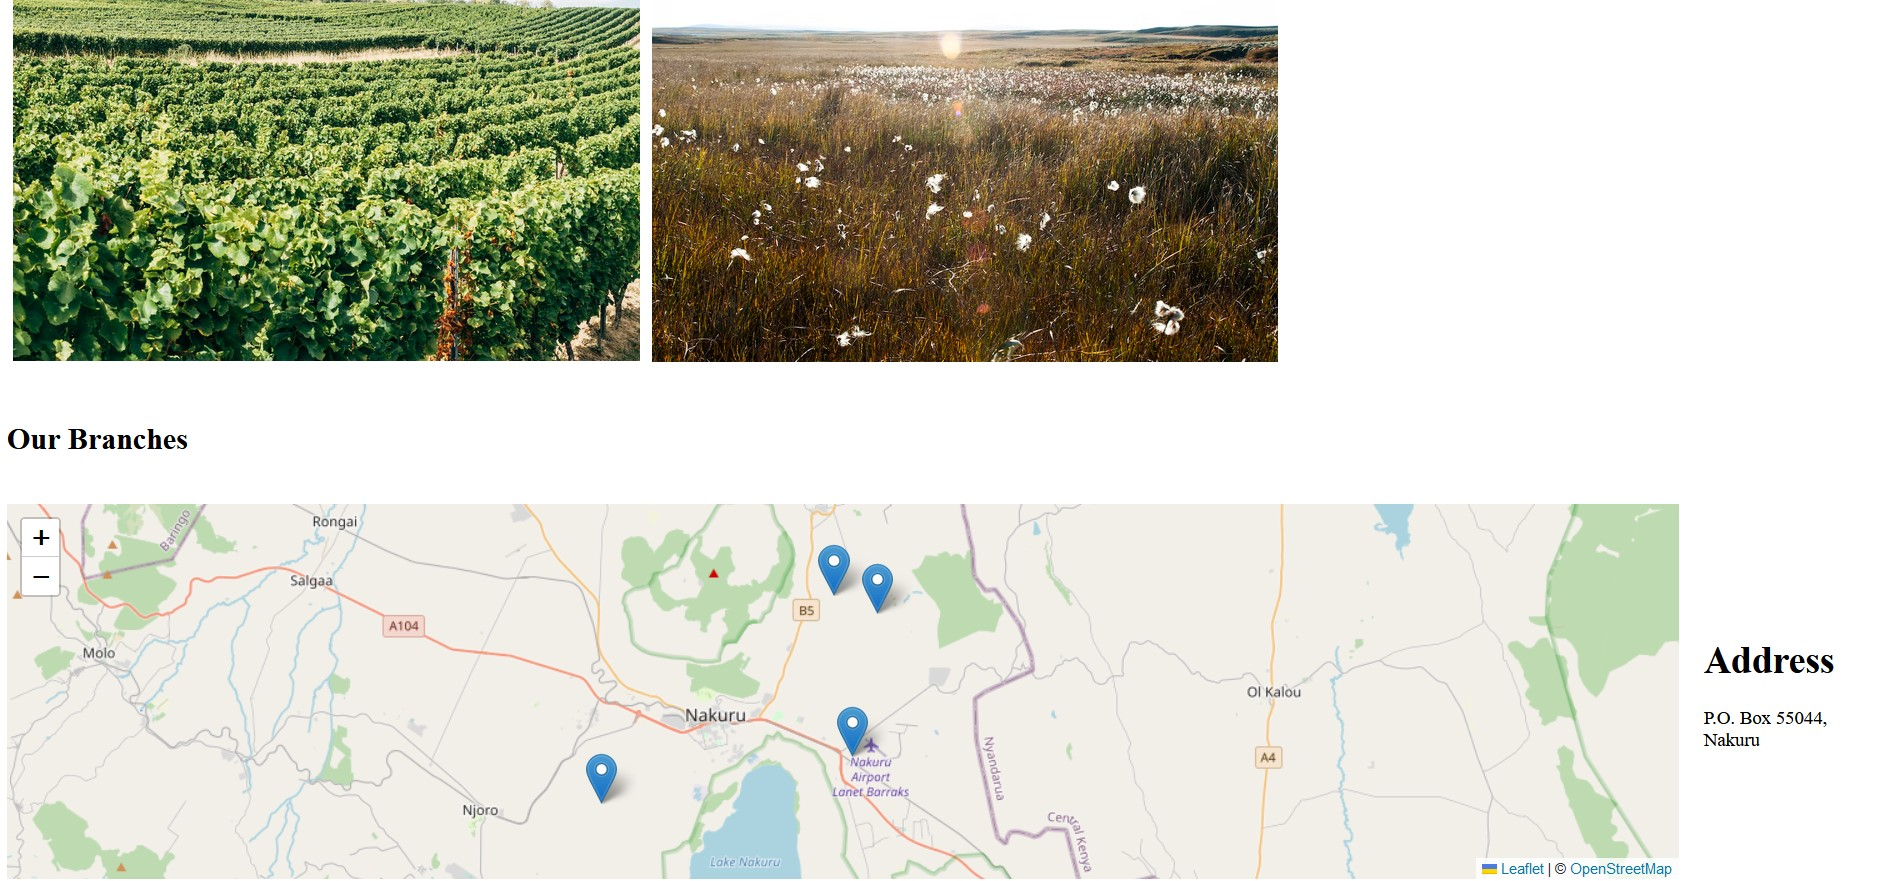
\includegraphics{../images/embedded.jpg}

``How are we able to align the webmap to the left and also make other text stand aside to it?'' This is all thanks to the CSS property \texttt{display:\ flex}. \texttt{display} is a CSS property that deals with how HTML elements are displayed.

The \texttt{display} property aligns a HTML element to fill or shrink according to the space available within its assigned portion in the webpage. On the other hand, the CSS property \texttt{padding-left} just creates space all around the element, thus creating a neat space between the Leaflet map and the address text. Removing this will just make the address text and the Leaflet map touch each other edge to edge. The inspiration to use all these CSS properties and values in placing HTML elements side-by-side emanated from this \href{https://www.w3docs.com/snippets/css/how-to-vertically-align-text-next-to-an-image.html?utm_source=pocket_saves}{example}.

Having done the above, you can consider you are as good a Leaflet mapper to undertake any task! Later on, in \protect\hyperlink{standard-website-with-leaflet-project}{Chapter 13}, we shall see how to insert a Leaflet map in a more sophisticated website. This was just a gentle introduction.

\hypertarget{summary-3}{%
\section{Summary}\label{summary-3}}

This chapter has introduced you on how you can use CSS to customize the appearance and positioning of your webmap. You have also encountered the use of \texttt{for} loop in JavaScript code to retrieve geospatial information, particularly from arrays. Here are some of the take aways from this chapter.

\begin{itemize}
\item
  Leaflet maps can be embedded inside a website as demonstrated in the dummy Pro-GMO webpage.
\item
  One can use \texttt{for} loops to iterate over elements from an array and retrieve geospatial information. In this chapter, the \texttt{for} loop was used to retrieve both latitude-longitude coordinates and text from the \texttt{branches} array variable.
\item
  We can use CSS elements, such as \texttt{display} and \texttt{padding-left} to position and define how a webmap shall be displayed on our webpage.
\end{itemize}

\hypertarget{using-geojson-in-leaflet}{%
\chapter{Using GeoJSON in Leaflet}\label{using-geojson-in-leaflet}}

\hypertarget{creating-a-.geojson-file}{%
\section{\texorpdfstring{Creating a \texttt{.geojson} file}{Creating a .geojson file}}\label{creating-a-.geojson-file}}

So far, we have created a Leaflet map, added some aesthetics such as markers, and even embedded a map into a dummy website. Alright, the website wasn't even close to good, but the methodology should be the same when working with other fully functional and better looking websites. That may be enough to give you confidence to start as a webmapper but not so fast! There is still more territory to cover! I would like to introduce another format of storing geospatial information --the use of \texttt{.geojson} files.

\hypertarget{what-are-.geojson-files}{%
\section{\texorpdfstring{What are \texttt{.geojson} files?}{What are .geojson files?}}\label{what-are-.geojson-files}}

\texttt{.geojson} files, according to the GIS leader ESRI, are an \href{https://doc.arcgis.com/en/arcgis-online/reference/geojson.htm}{open standard geospatial data interchange format} that represents simple geographic features and their non-spatial attributes. GeoJSON is based on the JavaScript Object Notation (JSON) file format which is a lightweight data exchange format that is easily interpretable by both man and machine. In very few instances does any data format please both sides of the divide but JSON does, and this \href{https://www.oracle.com/ke/database/what-is-json/}{site} provides examples. Anyway, just like you can tell from the name, JSON is based on the JavaScript programming language. If you have worked with JavaScript before, it looks very much like a data format based on dictionaries. In essence, JSON is a large dictionary holding other \emph{dictionaries} of data within it. A GeoJSON is a JSON file that follows a certain structure and has spatial index and geometry specifications in it. See this \href{https://datascience.aero/geospatial-data-representation-the-geojson-format/}{website} for a GeoJSON example.

An example of a GeoJSON file format structure is shown below:

\begin{verbatim}
{
  "type": "FeatureCollection",
  "features": [
    {
      "type": "Feature",
      "properties": {
        "City": "Nairobi",
        "Population": "4, 300, 000"
      },
      "geometry": {
        "coordinates": [
          36.80617598261199,
          -1.2868825246637812
        ],
        "type": "Point"
      }
    },
    {
      "type": "Feature",
      "properties": {
        "City": "Kisumu",
        "Population": "610, 082"
      },
      "geometry": {
        "coordinates": [
          34.738718987625106,
          -0.10390483386935045
        ],
        "type": "Point"
      }
    },
    ---snip----
\end{verbatim}

Below is an example of a \href{https://www.oracle.com/ke/database/what-is-json/}{json file structure}.

\begin{verbatim}
{

"Influencers" :   [ 
{
 "name" : "Jaxon", 
 "age" : 42, 
 "Works At" : "Tech News"
}

{
 "name" : "Miller", 
 "age" : 35
 "Works At" : "IT Day"
}

] 
}
\end{verbatim}

\hypertarget{why-geojson}{%
\section{\texorpdfstring{Why \texttt{geojson}?}{Why geojson?}}\label{why-geojson}}

Yours truly could be wrong, but one advantage of \texttt{geojson} and \texttt{json} is that it's minimal on size compared to shapefiles and it is also more portable. Shapefiles are dependent on other data formats that accompany it, such as \texttt{.shx}, \texttt{.dbf}, \texttt{.prj} which provide auxillary geospatial orientation, metadata, and attributes. On the other hand, GeoJSON and JSON formats will come as single files but will still as much data as all the components of a shapefile (\texttt{.shx}, \texttt{.dbf}, and \texttt{.prj}) put together.

So when do I use shapefiles vis a vis GeoJson? If you want to work with geospatial data in a web interface, \texttt{geojson} is the way to go. Period.

\hypertarget{creating-a-geojson-file}{%
\section{Creating a geojson file}\label{creating-a-geojson-file}}

It may look intimidating to create a GeoJSON file without hardly making any errors, and it actually is, but luckily the \href{https://geojson.io/\#map=2/0/20}{geojson.io} website does the heavy lifting for us. We shall head over to it and create a \texttt{geojson} file of some cities and their population.

First, of all, the website looks like below. Talk of a cool global map powered by Mapbox.

\begin{Shaded}
\begin{Highlighting}[]
\NormalTok{knitr}\SpecialCharTok{::}\FunctionTok{include\_graphics}\NormalTok{(}\FunctionTok{rep}\NormalTok{(}\StringTok{"D:/gachuhi/my{-}leaflet/images/mapbox{-}front.jpg"}\NormalTok{))}
\end{Highlighting}
\end{Shaded}

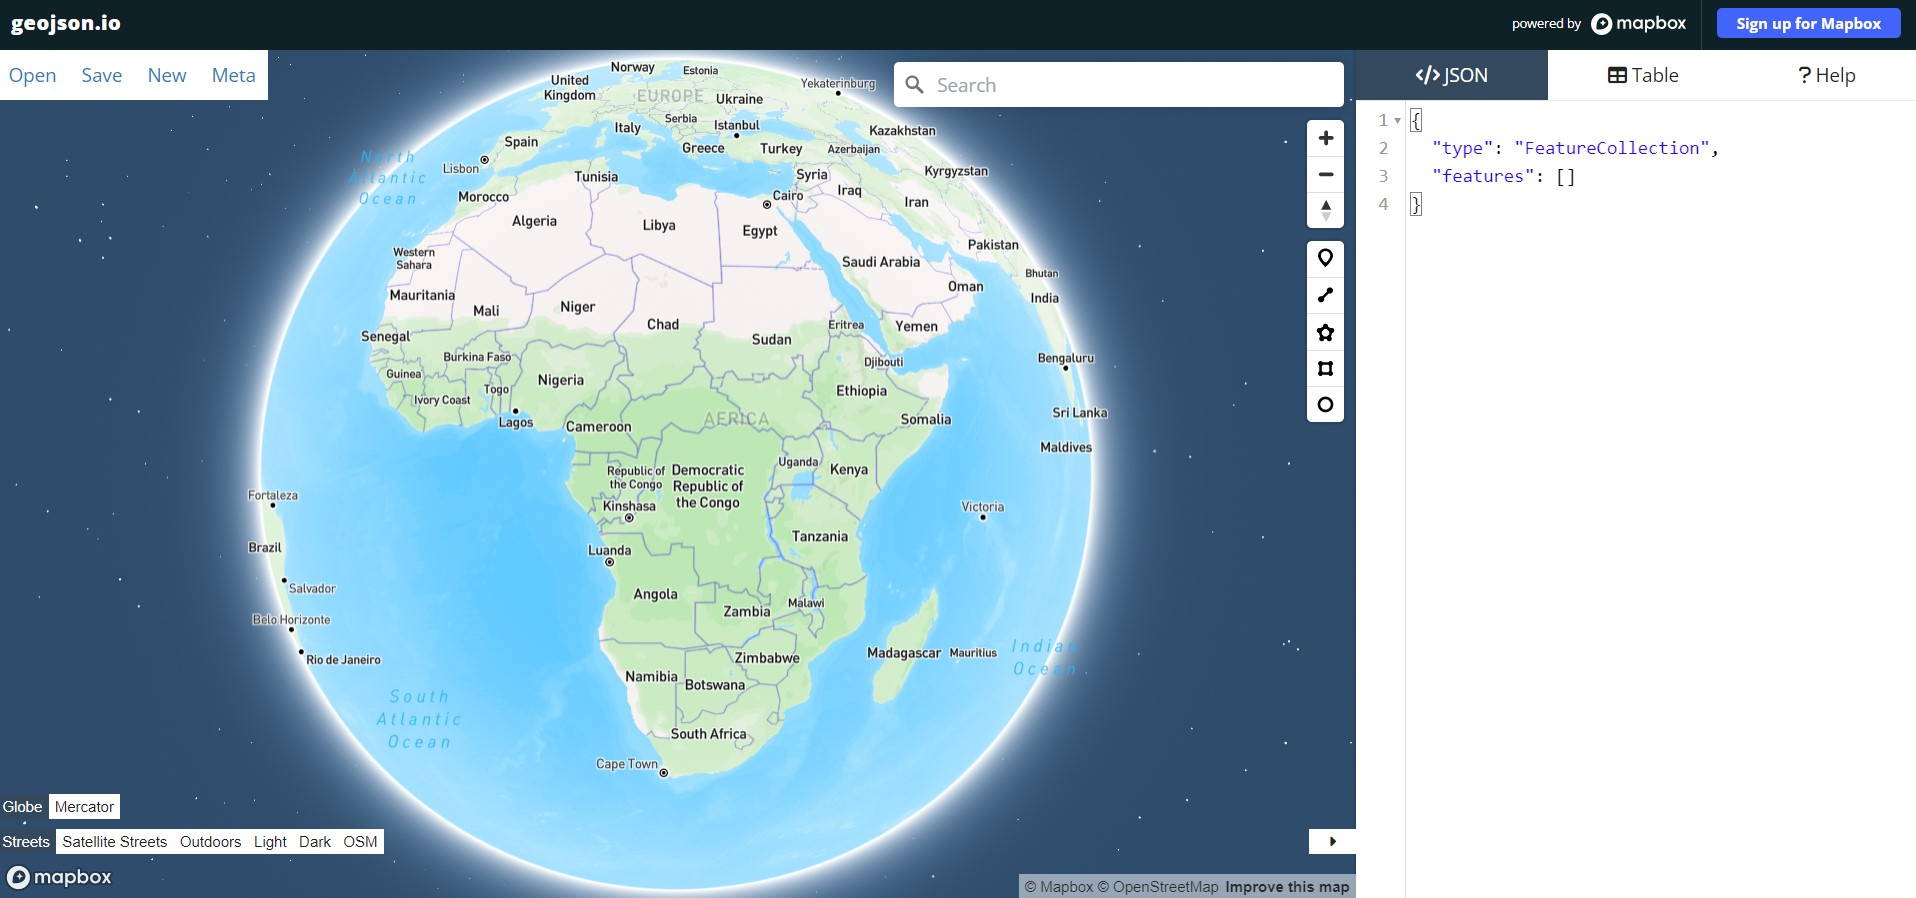
\includegraphics{../images/mapbox-front.jpg}

On your right, under the \textbf{\textless/\textgreater JSON} tab, the Mapbox folks have already given you a head start by indicating what feature type and features will go into your \texttt{geojson} file. These are important as any website uses these keywords when parsing information from the GeoJSON file. Zoom to Kenya and click a point on top of the Nairobi dot pin, like shown below. Use the highlighted pin in the image below to create a marker over Nairobi.

\begin{Shaded}
\begin{Highlighting}[]
\NormalTok{knitr}\SpecialCharTok{::}\FunctionTok{include\_graphics}\NormalTok{(}\FunctionTok{rep}\NormalTok{(}\StringTok{"D:/gachuhi/my{-}leaflet/images/nairobi{-}pin.jpg"}\NormalTok{))}
\end{Highlighting}
\end{Shaded}

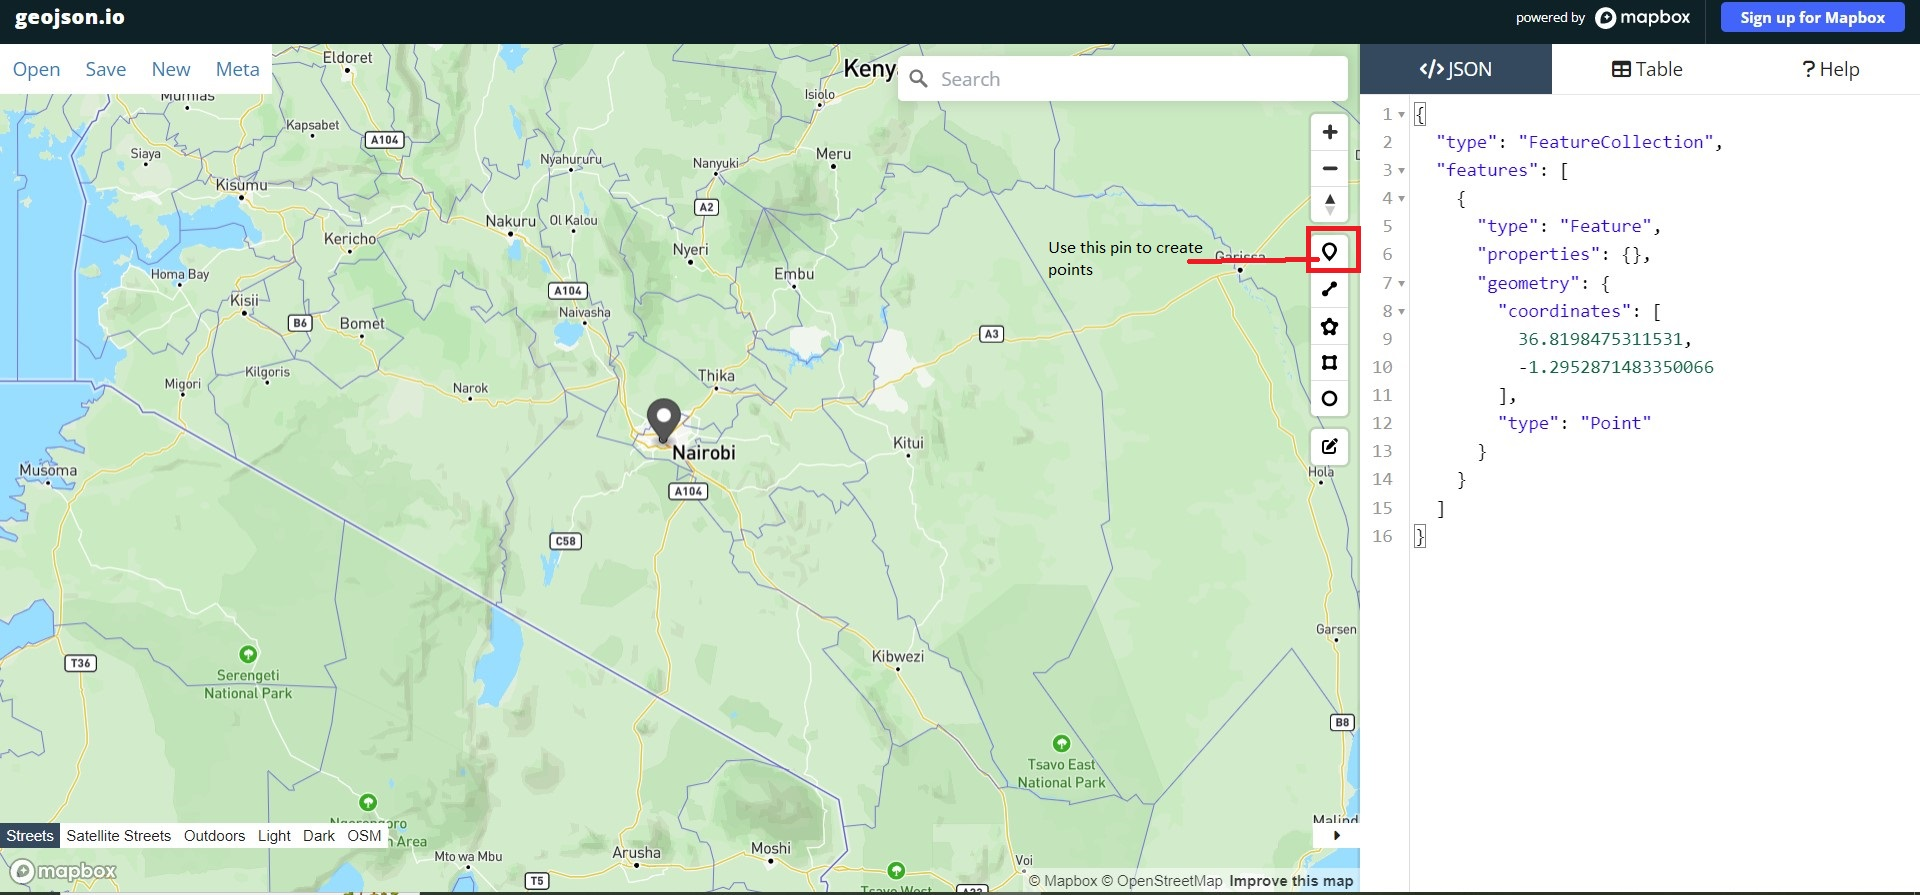
\includegraphics{../images/nairobi-pin.jpg}

By doing so, you will realize that a new dictionary of \texttt{type}, \texttt{properties} and \texttt{geometry} appears within the \textbf{features} list. These new keys provide the additional spatial and geometry data in their values which a website uses to place them at their appropriate locations on the webmap.

Now move over to the \textbf{Table} tab and click new column as shown below.

\begin{Shaded}
\begin{Highlighting}[]
\NormalTok{knitr}\SpecialCharTok{::}\FunctionTok{include\_graphics}\NormalTok{(}\FunctionTok{rep}\NormalTok{(}\StringTok{"D:/gachuhi/my{-}leaflet/images/table.jpg"}\NormalTok{))}
\end{Highlighting}
\end{Shaded}

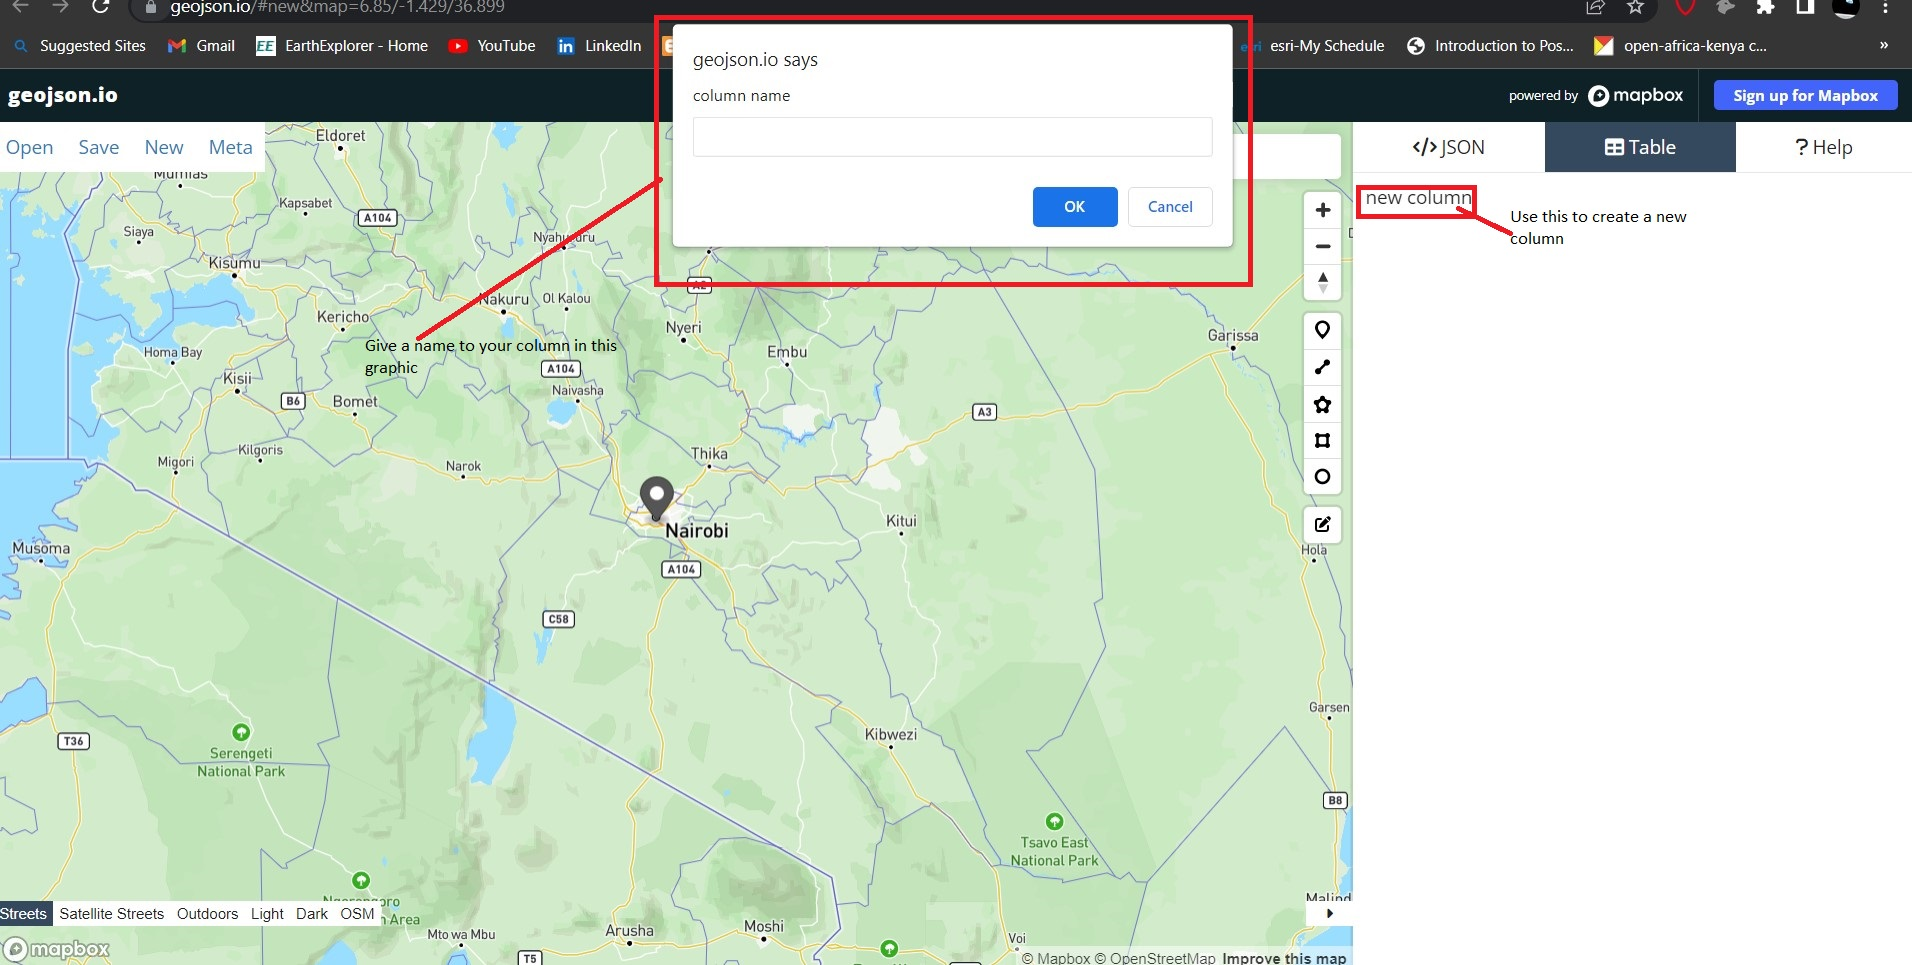
\includegraphics{../images/table.jpg}

Click on it and in the graphic that appears, give your column the name \textbf{City}. Click \textbf{Ok} and in the table cell that appears, type \textbf{Nairobi}.

\begin{Shaded}
\begin{Highlighting}[]
\NormalTok{knitr}\SpecialCharTok{::}\FunctionTok{include\_graphics}\NormalTok{(}\FunctionTok{rep}\NormalTok{(}\StringTok{"D:/gachuhi/my{-}leaflet/images/nairobi{-}named.jpg"}\NormalTok{))}
\end{Highlighting}
\end{Shaded}

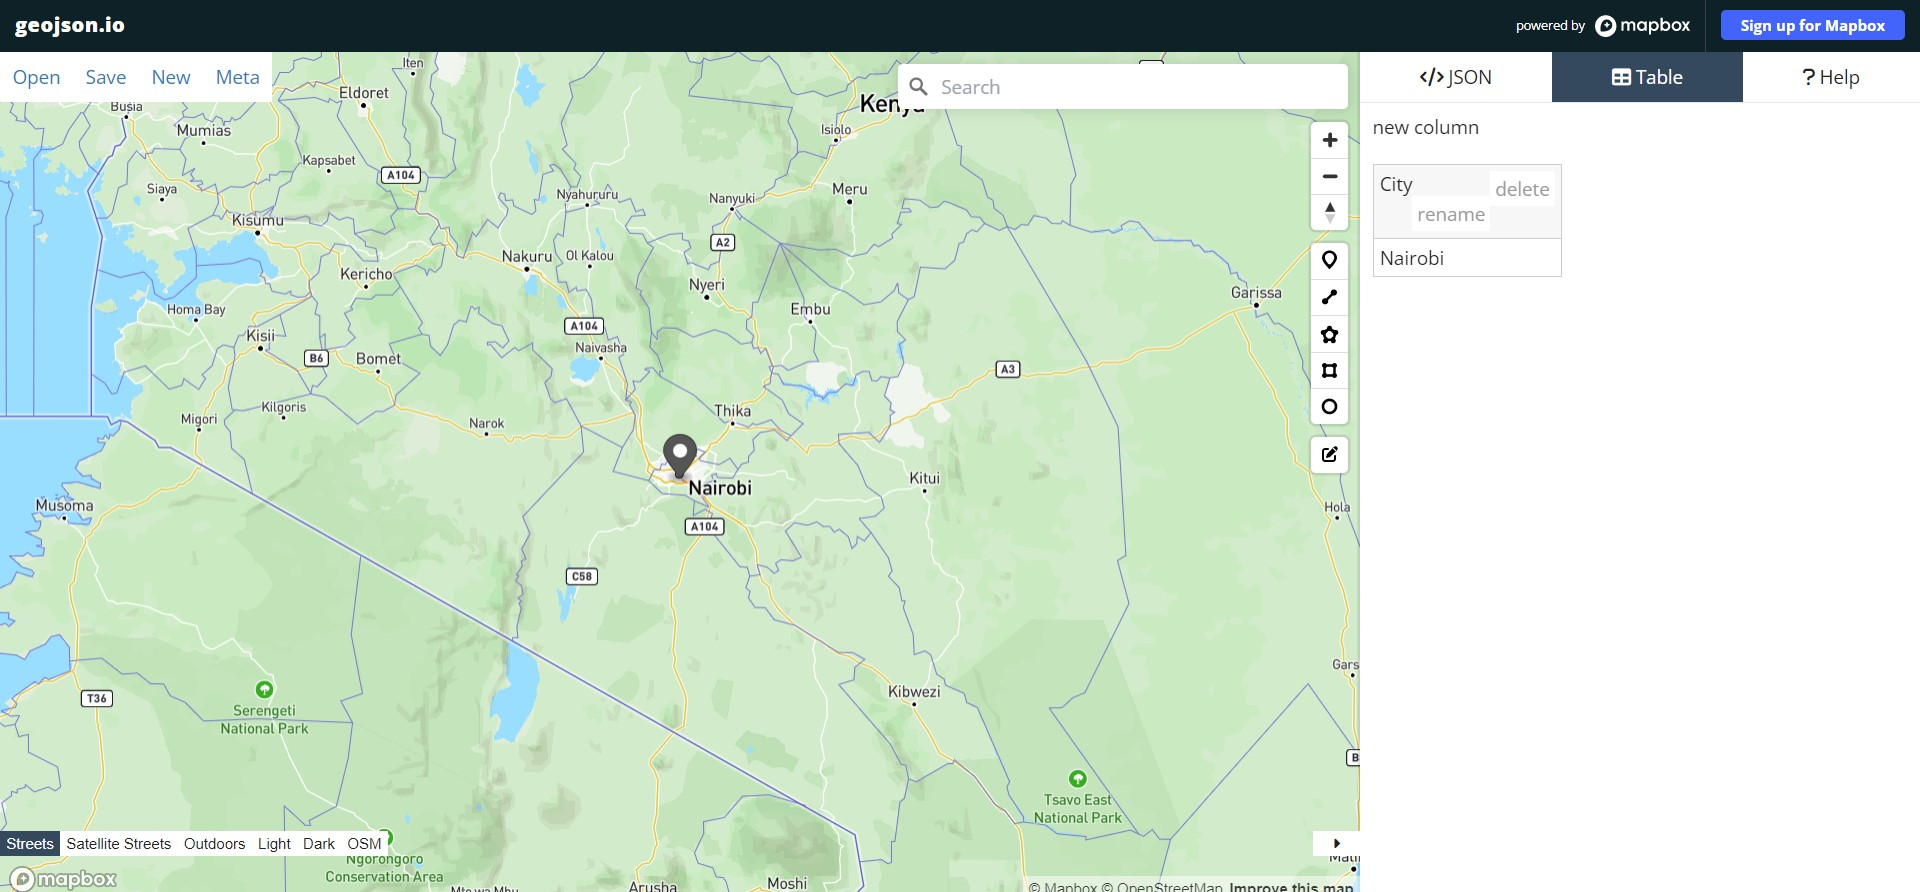
\includegraphics{../images/nairobi-named.jpg}

Now create a new pin over \emph{Kisumu} and two things will happen: a new dictionary will appear below that of Nairobi and a new table row will appear in the \textbf{Table} tab. Create pins over the following cities: Mombasa, Nakuru, Nyeri, Machakos and Malindi. Legally speaking, only the first four are cities by law, the rest are just towns but for the sake of this tutorial, let's corporately refer to them as cities.

\begin{Shaded}
\begin{Highlighting}[]
\NormalTok{knitr}\SpecialCharTok{::}\FunctionTok{include\_graphics}\NormalTok{(}\FunctionTok{rep}\NormalTok{(}\StringTok{"D:/gachuhi/my{-}leaflet/images/cities{-}named.jpg"}\NormalTok{))}
\end{Highlighting}
\end{Shaded}

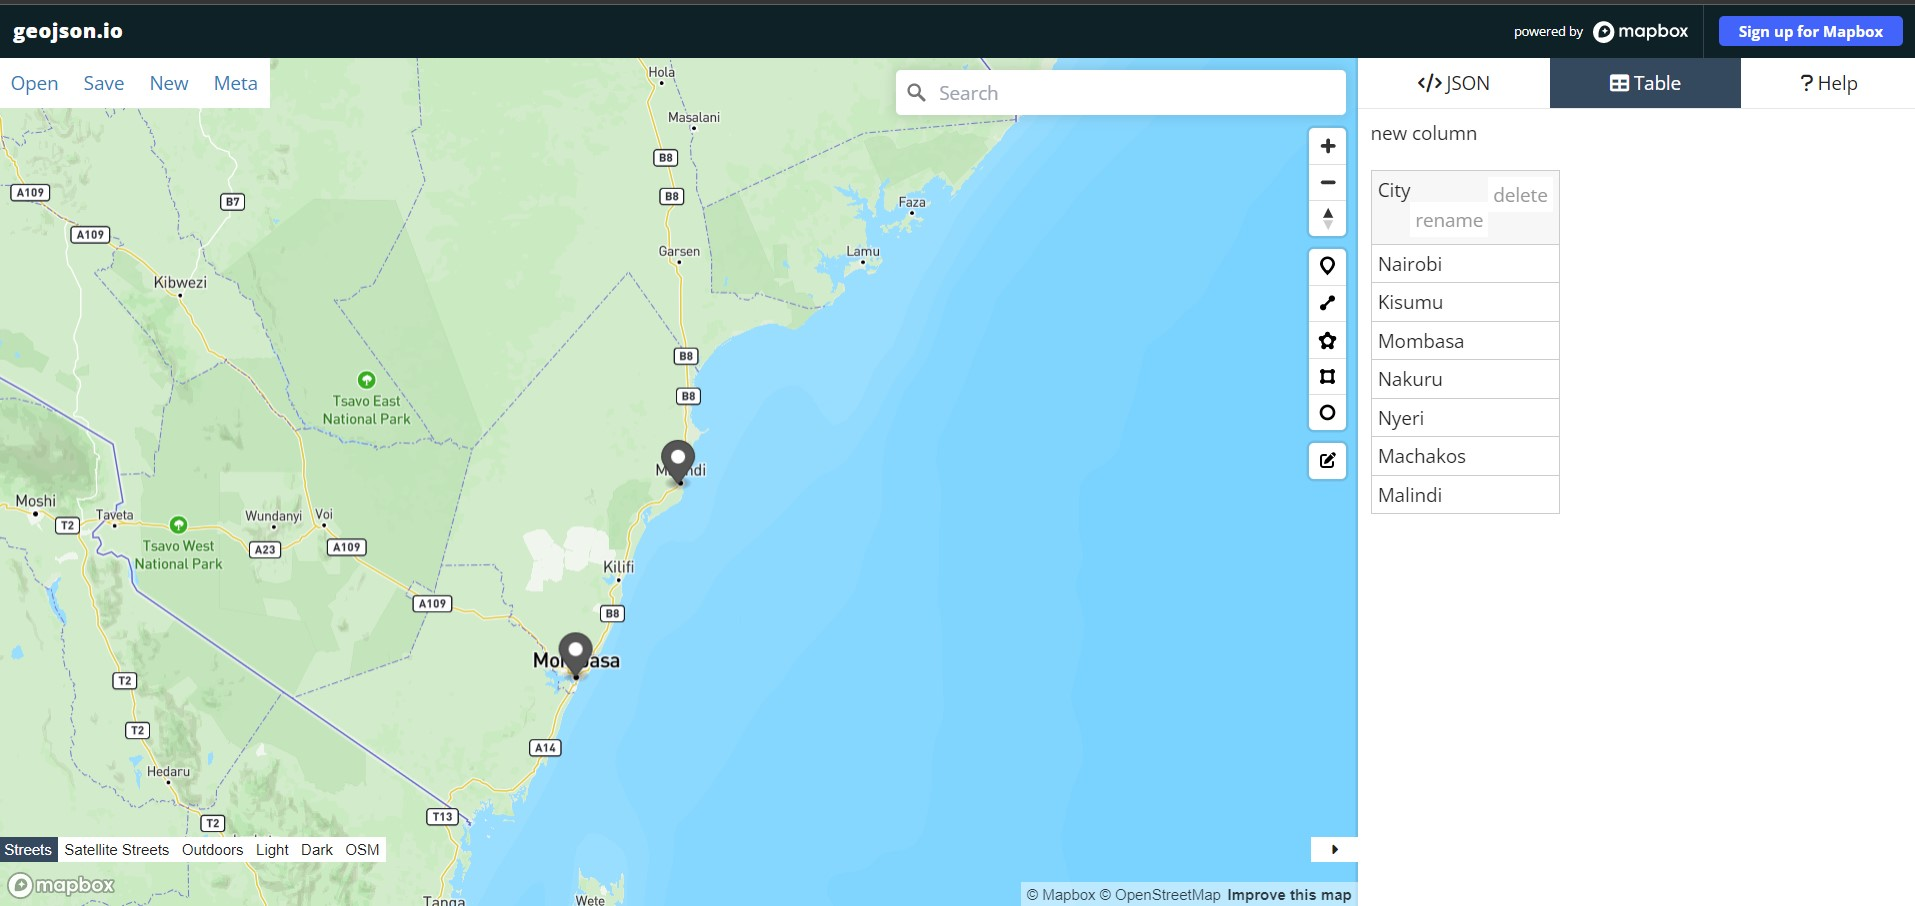
\includegraphics{../images/cities-named.jpg}

Alright, one process down, one more to go. We will fill these cities with their population statistics. Create a new column with the heading \textbf{Population}. Fill each of the cities with the following statistics.

\begin{Shaded}
\begin{Highlighting}[]
\FunctionTok{read.csv}\NormalTok{(}\StringTok{"D:/gachuhi/my{-}leaflet{-}vs/data/points.csv"}\NormalTok{)[ , }\DecValTok{1}\SpecialCharTok{:}\DecValTok{2}\NormalTok{]}
\end{Highlighting}
\end{Shaded}

\begin{verbatim}
##       City  Population
## 1  Nairobi 4, 300, 000
## 2   Kisumu    610, 082
## 3  Mombasa 1, 440, 000
## 4   Nakuru    422, 000
## 5    Nyeri    759, 164
## 6 Machakos 1, 422, 000
## 7  Malindi    119, 859
\end{verbatim}

Once done, head over to the top left of the \href{http://geojson.io/}{geojson.io} website, and click \textbf{Save}. A list of options will appear, click on save as \textbf{geojson}. It should appear somewhere in your \emph{Downloads} directory.

\begin{Shaded}
\begin{Highlighting}[]
\NormalTok{knitr}\SpecialCharTok{::}\FunctionTok{include\_graphics}\NormalTok{(}\FunctionTok{rep}\NormalTok{(}\StringTok{"D:/gachuhi/my{-}leaflet/images/geojson{-}save.jpg"}\NormalTok{))}
\end{Highlighting}
\end{Shaded}

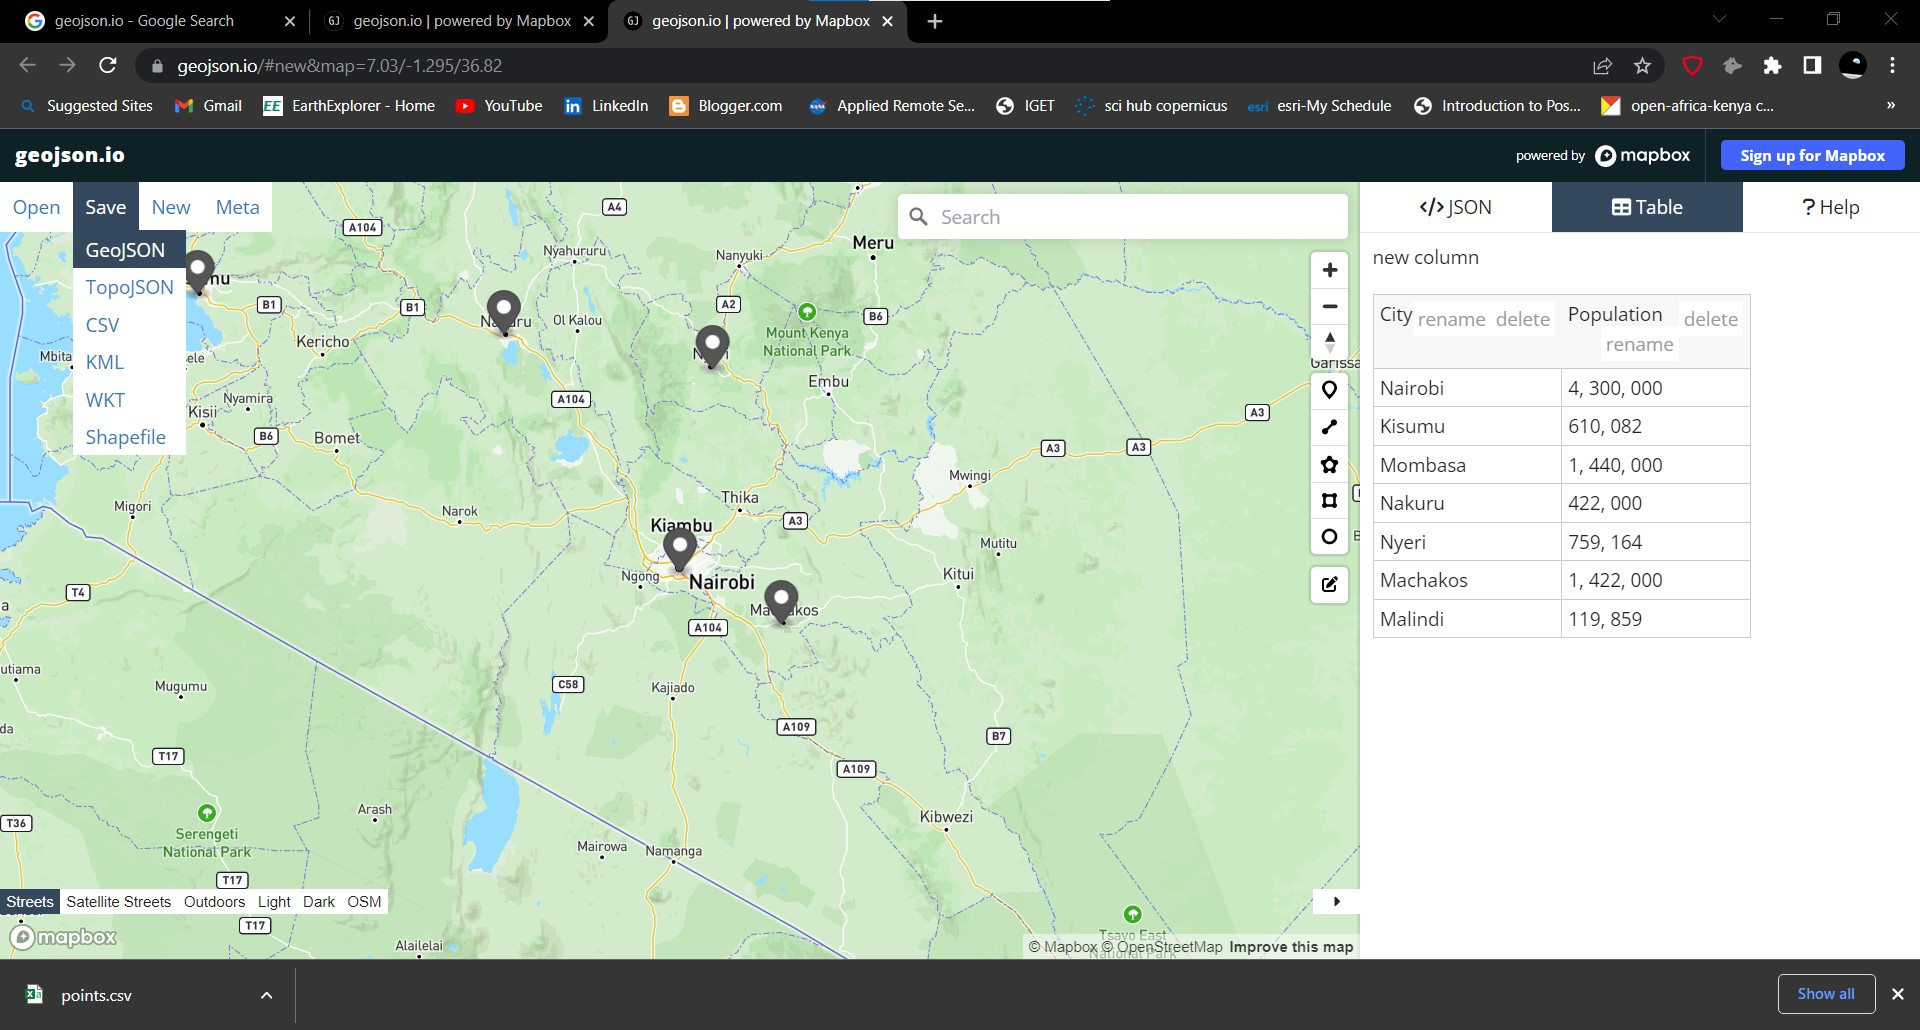
\includegraphics{../images/geojson-save.jpg}

\hypertarget{saving-the-geojson-to-github}{%
\section{Saving the Geojson to Github}\label{saving-the-geojson-to-github}}

Now, based on experience, loading a local Geojson file (one within your computer directory) to JavaScript is a painful, if not near impossible experience. The resulting errors had to with servers or something. To get a way around this and still be able to display \texttt{.geojson} data in Leaflet, the GeoJson file had to be stored on an online server, in this case, Github. We would love to show you how to save data on Github, but this would make this chapter way too long. Therefore, and with sincere apologies, it would be best if you googled it out. Nevertheless, here is the \href{https://raw.githubusercontent.com/sammigachuhi/geojson_files/main/cities-geojson.geojson}{GeoJSON file}, and it will come in handy in the last two sub-chapters of this exercise.

\hypertarget{loading-the-geojson-into-leaflet}{%
\section{Loading the GeoJSON into Leaflet}\label{loading-the-geojson-into-leaflet}}

As they always say, there are many ways of killing a rat. There are around three ways in which to load GeoJson data into Leaflet, at least from our discovery. We shall start with the easiest and most unreliable to what we consider the best. Let start with the easy one, loading a \texttt{.geojson} file from within our Javascript file itself.

\hypertarget{the-easy-way}{%
\subsection{The easy way}\label{the-easy-way}}

First of all create a blank JavaScript file called \texttt{geojson.js}. Thereafter, go to your \texttt{map.html} file which you had created last in \protect\hyperlink{setting-the-superstructure}{Chapter 2}. Open it. Within the \texttt{\textless{}script\textgreater{}} tag of the \texttt{\textless{}body\textgreater{}} element, change the \texttt{src} attribute to read \texttt{"geojson.io"} like below.

\begin{verbatim}
<!DOCTYPE html>
<html lang="en">
    <head>
        -- snip ---
    </head>
    <body>
        <div id="myMap">
            <script src="geojson.js">
            </script> 
        </div>  
        
    </body>
</html>
\end{verbatim}

Alright. Head over to your \texttt{geojson.js} and as always, add the Leaflet classes \texttt{L.map} and \texttt{L.tileLayer}. We set the view of our new Leaflet map to that of Nairobi. Your blank \texttt{geojson.js} should now be filled with the below code.

\begin{verbatim}
var map = L.map('myMap').setView([-1.295287148, 36.81984753], 7);

L.tileLayer('https://tile.openstreetmap.org/{z}/{x}/{y}.png', {
    maxZoom: 19,
    attribution: '&copy; <a href="http://www.openstreetmap.org/copyright">OpenStreetMap</a>'
}).addTo(map);
\end{verbatim}

Okay. Head over to \url{geojson.io} website and right under the \textbf{\textless/\textgreater JSON} you will see a copy icon.

\begin{Shaded}
\begin{Highlighting}[]
\NormalTok{knitr}\SpecialCharTok{::}\FunctionTok{include\_graphics}\NormalTok{(}\FunctionTok{rep}\NormalTok{(}\StringTok{"D:/gachuhi/my{-}leaflet/images/geojson{-}copy.jpg"}\NormalTok{))}
\end{Highlighting}
\end{Shaded}

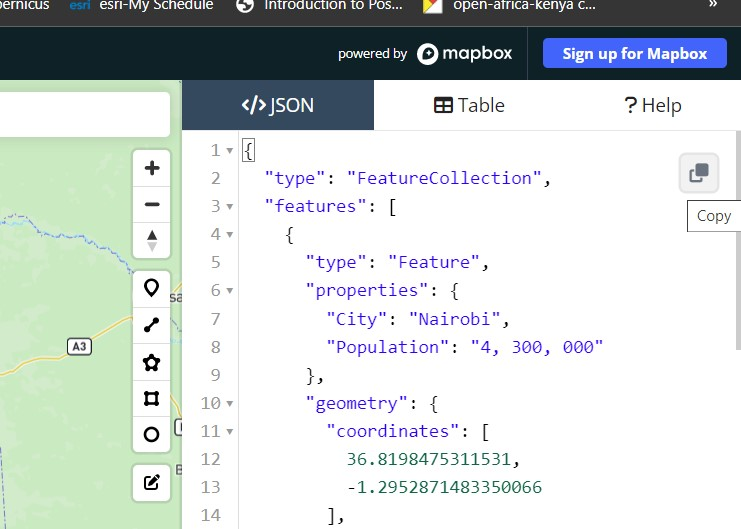
\includegraphics{../images/geojson-copy.jpg}
Click it and paste the json code into your \texttt{geojson.js} file right above the other \texttt{L.map} and \texttt{L.tileLayer} classes. The contents of your \texttt{geojson.js} should look like below.

\begin{verbatim}
var cities = {
    "type": "FeatureCollection",
    "features": [
      {
        "type": "Feature",
        "properties": {
          "City": "Nairobi",
          "Population": "4, 300, 000"
        },
        "geometry": {
          "coordinates": [
            36.8198475311531,
            -1.2952871483350066
          ],
          "type": "Point"
        }
      },
      -- snip ---
      {
        "type": "Feature",
        "properties": {
          "City": "Malindi",
          "Population": "119, 859"
        },
        "geometry": {
          "coordinates": [
            40.10521499751357,
            -3.2138767356491655
          ],
          "type": "Point"
        }
      }
    ]
  }


var map = L.map('myMap').setView([-1.295287148, 36.81984753], 7);

L.tileLayer('https://tile.openstreetmap.org/{z}/{x}/{y}.png', {
    maxZoom: 19,
    attribution: '&copy; <a href="http://www.openstreetmap.org/copyright">OpenStreetMap</a>'
}).addTo(map);
\end{verbatim}

Refresh your \texttt{map.html}. It's a map of Kenya alright, but none of our \texttt{.geojson} features appear yet. We are about to change that. Leaflet offers the \texttt{L.geoJSON} class to add GeoJSON data to a map. The class name speaks for itself and therefore let's use it to add our GeoJSON features. Add the following code below the other Leaflet map class layers.

\begin{verbatim}
L.geoJSON(cities).addTo(map);
\end{verbatim}

Refresh your \texttt{map.html}. The GeoJSON features should now appear at their exact locations.

\begin{Shaded}
\begin{Highlighting}[]
\NormalTok{knitr}\SpecialCharTok{::}\FunctionTok{include\_graphics}\NormalTok{(}\FunctionTok{rep}\NormalTok{(}\StringTok{"D:/gachuhi/my{-}leaflet/images/geojson{-}leaflet.jpg"}\NormalTok{))}
\end{Highlighting}
\end{Shaded}

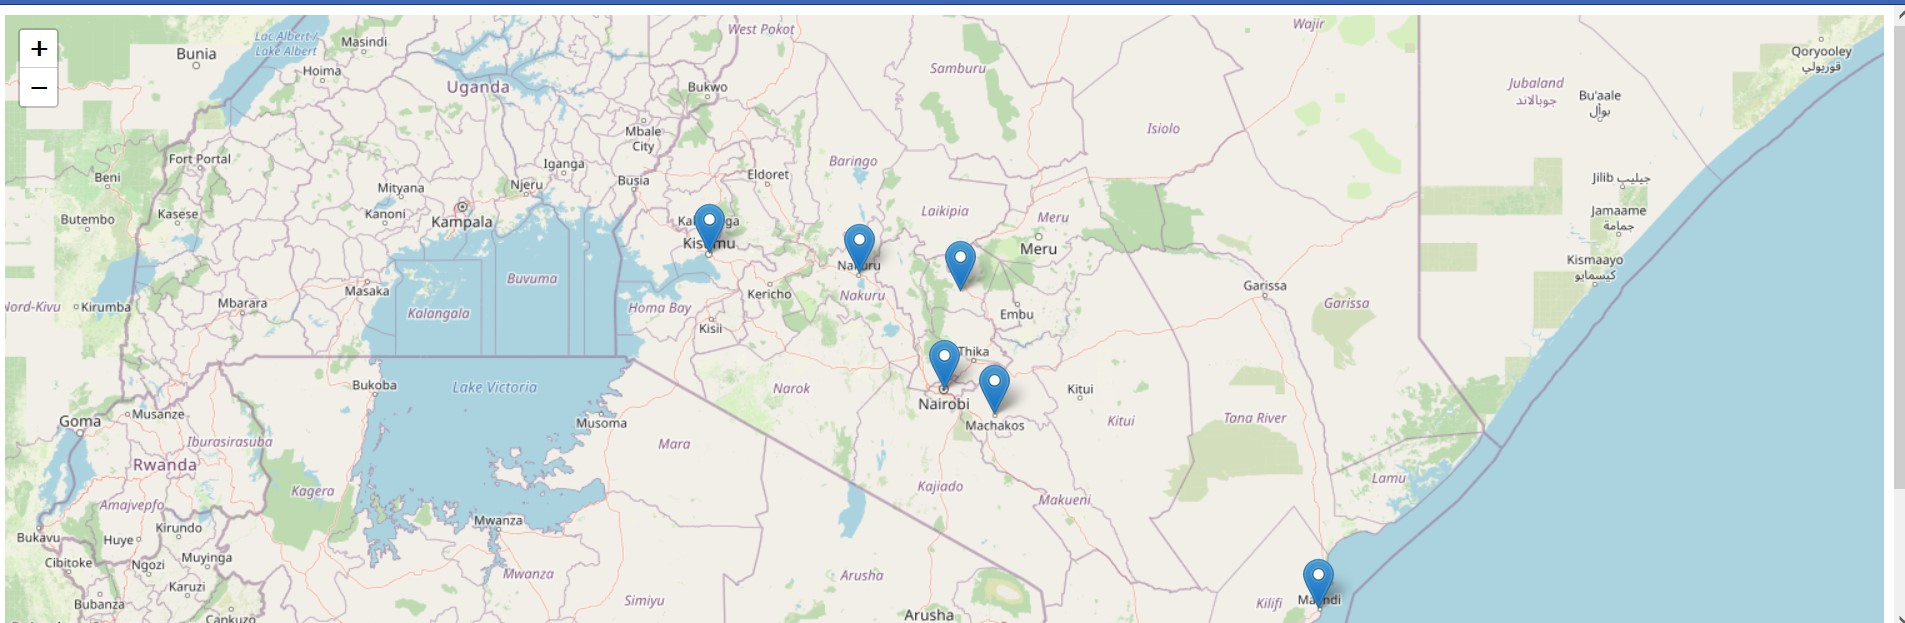
\includegraphics{../images/geojson-leaflet.jpg}

How about if we made the markers more interactive? Say, like they display popups as we did in \protect\hyperlink{a-marker-with-a-popup}{Chapter 3}? We would like the city names to appear upon a user's click on the markers. Easy. Just create a function that does so as in the logic provided \href{https://leafletjs.com/reference.html\#geojson}{here}. We customized it to our case to make sure it references to the \texttt{City} key which is part of the dictionary attached to the \texttt{properties} key.

\begin{verbatim}
L.geoJSON(cities).bindPopup(function (layer) {
    return layer.feature.properties.City;
}).addTo(map);
\end{verbatim}

\begin{Shaded}
\begin{Highlighting}[]
\NormalTok{knitr}\SpecialCharTok{::}\FunctionTok{include\_graphics}\NormalTok{(}\FunctionTok{rep}\NormalTok{(}\StringTok{"D:/gachuhi/my{-}leaflet/images/geojson{-}names.jpg"}\NormalTok{))}
\end{Highlighting}
\end{Shaded}

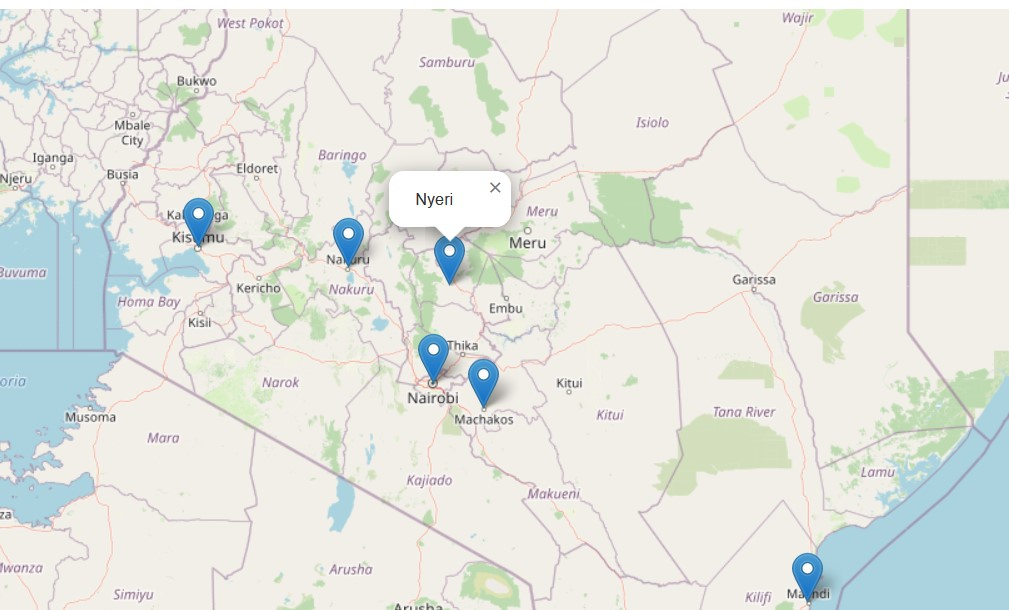
\includegraphics{../images/geojson-names.jpg}

There is one issue with this method. If we have a very long GeoJSON data structure, it will clatter our JavaScript file. We only worked with seven cities, but it is very common to work with data holding hundreds and even thousands of dictionaries. That would make your JavaScript file stretch to \emph{ad infitum}.

This brings us to the other two methods, that of using the \textbf{Ajax} plugin and using the \textbf{Fetch} Application Programming Interface (API). Don't let the words scare you. Take a break, grab a glass of water and come back.

\hypertarget{using-the-ajax-plugin}{%
\subsection{Using the Ajax Plugin}\label{using-the-ajax-plugin}}

As the term `plugin' suggests, this is an extension that offers additional functions to the core Leaflet plugin. The Ajax plugin is available from this \href{https://github.com/calvinmetcalf/leaflet-ajax/archive/refs/heads/gh-pages.zip}{link}. Download it to your directory and preferably within the same directory as your \texttt{map.html} and \texttt{geojson.js}. Alright. Right under the \texttt{src} for \texttt{leaflet.js} in your \texttt{map.html}, add the following \texttt{\textless{}script\textgreater{}} tag.

\begin{verbatim}
    <head>
        -- snip --
        <script src="leaflet-ajax-gh-pages\dist\leaflet.ajax.js"></script>
        
    </head>
    -- snip --
\end{verbatim}

This file will allow you to add \texttt{.geojson} files to your Leaflet map. However, there is a catch. Both the Ajax and Fetch APIs only work with GeoJson file formats saved on a web server. Based on experience, they will not work with local GeoJson files. As a work around, we saved our GeoJSON file to Github. For convenience, here is the \href{https://raw.githubusercontent.com/sammigachuhi/geojson_files/main/cities-geojson.geojson}{link} again to the raw file we had initially created from geojson.io.

We shall call our GeoJSON file from Github using Ajax as shown in the code below. Please remember to comment out your \texttt{var\ cities} and \texttt{L.geoJSON} using \texttt{\textbackslash{}\textbackslash{}} because they are irrelevant in this particular case.

\begin{verbatim}
var geojsonLayer = new L.geoJson.ajax("https://raw.githubusercontent.com/sammigachuhi/geojson_files/main/cities-geojson.geojson").addTo(map);
\end{verbatim}

Your map should now show the markers of our cities. If you are hawk eyed, you may have noticed that the syntax for Ajax is different from that of the earlier \texttt{L.geoJSON} from Leaflet. Starting with the latter, we have instead used \texttt{L.geoJson} and unlike in the Ajax creator's website where they used \texttt{var\ geojsonLayer\ =\ new\ L.GeoJSON.AJAX(\textless{}your-geojson-file\textgreater{})} we used the following syntax: \texttt{L.geoJson.ajax()} (ajax and geoJson beginning with small case). Actually, that's what worked after quite a lengthy web search.

Just like using \texttt{L.geoJSON}, we can also add popups after calling the \texttt{.ajax} method.

\begin{verbatim}
var geojsonLayer = new L.geoJson.ajax("https://raw.githubusercontent.com/sammigachuhi/geojson_files/main/cities-geojson.geojson")
    .bindPopup(function (layer) {
        return layer.feature.properties.City;
    }).addTo(map);
\end{verbatim}

Doing so should make the city names appear on clicking the markers on your Leaflet map.

\hypertarget{using-fetch-api}{%
\subsection{Using Fetch API}\label{using-fetch-api}}

Fetch API is a modern interface that allows you to make HTTP requests to servers from web browsers. In other words, it searches for a resource over the web, retrieves it, and brings it to you. Think of it as a dog in which you throw a saucer and tell your faithful hound: ``\emph{Sabretooth}, fetch!''. The dog runs after the saucer, grips it with its canines mid-air and quickly brings it back to you. Same case with Fetch API!

I had mentioned I will show you how to retrieve our Github stored GeoJSON data and I shall stick to the script! I shall also attempt to explain how this \emph{mysterious} \texttt{fetch} works.

First things first. The \texttt{fetch} function shall be called and passed to our Github url containing our GeoJSON text. Since \texttt{fetch} is an API, it retrieves data from Github.io --the server in this case--and brings it to our laptop the --the client. Enough IT. Let's write it down.

\begin{verbatim}
fetch("https://raw.githubusercontent.com/sammigachuhi/geojson_files/main/cities-geojson.geojson")
\end{verbatim}

Okay, next step. Once the server beams back the data to us, what do we do with it? According to \href{https://www.digitalocean.com/community/tutorials/js-fetch-api}{Digital Ocean}, the response is not \emph{actually} the data in the original format but rather \emph{a series of methods that can be used depending on what you want to do with the information}. This sounds downright confusing. Nevertheless, it is \emph{at least} crystal clear that the end goal is to have our fetched data in JSON format. Converting an object to JSON is done using the \texttt{json()} method. We parse \texttt{.json()} to a \texttt{then} method which is an asynchronous function\footnote{Asynchronous programming is a technique that enables your program to start a potentially long-running task and still be able to be responsive to other events while that task runs, rather than having to wait until that task has finished. Once that task has finished, your program is presented with the result. See \href{https://developer.mozilla.org/en-US/docs/Learn/JavaScript/Asynchronous/Introducing}{Mozilla}}. After the \texttt{fetch} function is successful, the object is stored in the \texttt{response} argument, which is in brackets, and then the function returns the result as a \texttt{json} object.

\begin{verbatim}
fetch("https://raw.githubusercontent.com/sammigachuhi/geojson_files/main/cities-geojson.geojson")
    .then(function(response) {
        return response.json()
    })
\end{verbatim}

After converting our response to JSON, it still needs to be processed further. Processed to what? To a GeoJSON file and subsequently add it to our Leaflet Map.

\begin{verbatim}
fetch("https://raw.githubusercontent.com/sammigachuhi/geojson_files/main/cities-geojson.geojson")
    .then(function(response) {
        return response.json()
    })
    .then(function(data) {
        L.geoJson(data).addTo(map);
    })
\end{verbatim}

We shall also add one more function --the \texttt{catch()} method. \texttt{catch()} is a method that returns an action if our response to the server has been rejected. Let's demonstrate all this.

\begin{verbatim}
fetch("https://raw.githubusercontent.com/sammigachuhi/geojson_files/main/cities-geojson.geojson")
    .then(function(response) {
        return response.json()
    })
    .then(function(data) {
        L.geoJson(data).addTo(map);
    })
    .catch(function(error) {
        console.log(`This is the error: ${error}`)
    })
\end{verbatim}

To see the \texttt{catch()} in action, omit the last letter in our url so that it reads \texttt{cities-geojson.geojso}. Yeah, you read it right. Just omit the letter `n' for now and reload your \texttt{map.html}. Right click the webmap page and click on \textbf{Inspect} in the small interface that appears. Head over to the console tab and see the error response. It should read like in the below image.

\begin{Shaded}
\begin{Highlighting}[]
\NormalTok{knitr}\SpecialCharTok{::}\FunctionTok{include\_graphics}\NormalTok{(}\FunctionTok{rep}\NormalTok{(}\StringTok{"D:/gachuhi/my{-}leaflet/images/catch{-}error.jpg"}\NormalTok{))}
\end{Highlighting}
\end{Shaded}

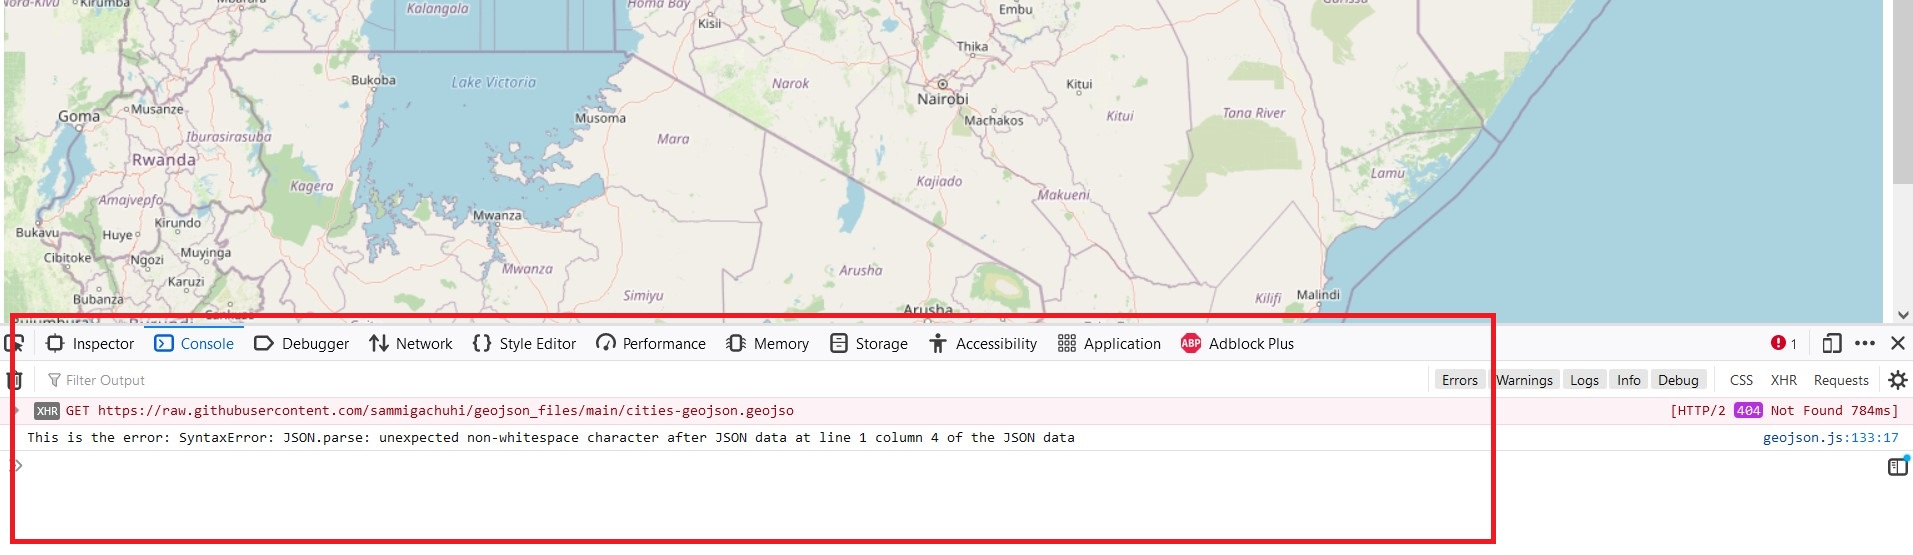
\includegraphics{../images/catch-error.jpg}

Restore the omitted letter `n' and reload your \texttt{map.html}. Your Leaflet map should have the city markers overlain just like in the case of using Ajax plugin or hardcoding the Geojson data into \texttt{var\ cities}. To stretch your Javascript skills further, we can shorten our code further by retaining the arguments \texttt{response}, \texttt{data} and \texttt{error} and using the arrow function \texttt{=\textgreater{}} to pass on the return statements, like so:

\begin{verbatim}
fetch("https://raw.githubusercontent.com/sammigachuhi/geojson_files/main/cities-geojson.geojson")
    .then((response) =>{
        return response.json()
    })
    .then((data) => {
        L.geoJson(data).addTo(map);
    })
    .catch((error) => {
        console.log(`This is the error: ${error}`)
    })
\end{verbatim}

It looks cryptic but don't cry! We have only ommitted the \texttt{function()} keyword and instead added \texttt{=\textgreater{}} between \texttt{function()} and the curly brackets \texttt{\{\textless{}code-to-run\textgreater{}\}} which is the function body aka where the magic happens. Just like when using Ajax, we can also add other functionalities to \texttt{L.geoJSON} within the \texttt{fetch} plugin. In here, and thanks to the use of template literals \texttt{(\textasciigrave{}\textasciigrave{})}, we can even add statements and refer to our GeoJson keys (and in some cases, even variables) using \texttt{\$\{\}}. Whatever is within the \texttt{\$\{\}} is executed and passed out as a string to the template literals.

\begin{verbatim}
fetch("https://raw.githubusercontent.com/sammigachuhi/geojson_files/main/cities-geojson.geojson")
    .then((response) =>{
        return response.json()
    })
    .then((data) => {
        L.geoJson(data).bindPopup((layer) => {
            return `City: ${layer.feature.properties.City},<br>
            Population: ${layer.feature.properties.Population}`}).addTo(map);
    })
    .catch((error) => {
        console.log(`This is the error: ${error}`)
    })
\end{verbatim}

In the \texttt{return} statement above, we added the HTML tag \texttt{\textless{}br\textgreater{}} to separate the \texttt{City} and \texttt{Population} keys from our GeoJSON. Doing so will return neat marker texts where the city name and population figures are in two separate lines.

Enough Javascript for a day!

\begin{Shaded}
\begin{Highlighting}[]
\NormalTok{knitr}\SpecialCharTok{::}\FunctionTok{include\_graphics}\NormalTok{(}\FunctionTok{rep}\NormalTok{(}\StringTok{"D:/gachuhi/my{-}leaflet/images/city{-}population.jpg"}\NormalTok{))}
\end{Highlighting}
\end{Shaded}

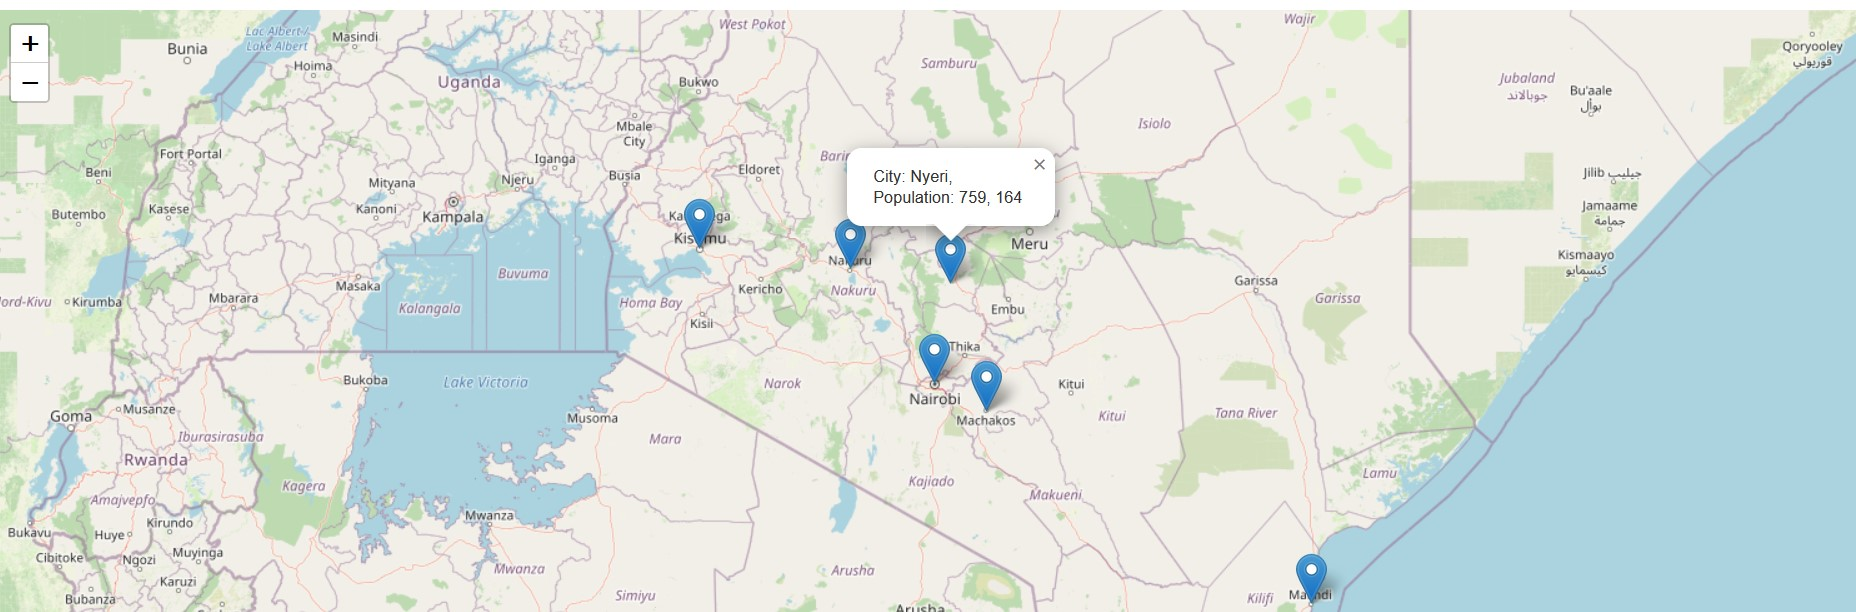
\includegraphics{../images/city-population.jpg}

Here are the \href{https://github.com/sammigachuhi/my-leaflet-project/tree/main/my-leaflet-code/chapter-5-geojson-leaflet}{full files} used in this chapter.

\hypertarget{summary-4}{%
\section{Summary}\label{summary-4}}

Who thought that simple GeoJSON files would be so complicated to load and see? Lets recap what we've learnt.

\begin{itemize}
\item
  GeoJSON files are an open standard geospatial data interchange format that represents simple geographic features and their nonspatial attributes.
\item
  GeoJSON is based on the JavaScript Object Notation (JSON) file format known for its lightweight nature.
\item
  GeoJSON files are the \emph{lingua franca} of working with spatial information on the web.
\item
  The \href{https://geojson.io/\#map=2/0/20}{geojson.io} website allows a user to create a GeoJSON file interactively and intuitively.
\item
  There are three main ways of loading a GeoJSON file in Leaflet. One is by hardcoding the dictionary of spatial attributes in a JavaScript file. This was the first method that we explored.
\item
  The other method is by using the Ajax plugin. We call Ajax into Leaflet by inserting into the \texttt{\textless{}head\textgreater{}} element the path to the extracted Ajax files.
\item
  The third and last method is through use of the \texttt{fetch} API. The \texttt{fetch} API searches for a resource over the web, retrieves it, and brings it to your computer.
\end{itemize}

\hypertarget{create-your-own-custom-markers}{%
\chapter{Create your own custom markers}\label{create-your-own-custom-markers}}

\hypertarget{setting-the-base}{%
\section{Setting the base}\label{setting-the-base}}

Hope you didn't trash away the cities we created in the last \protect\hyperlink{using-geojson-in-leaflet}{chapter}. In this chapter, we shall focus on creating your own custom markers. We love a clean job, so we will create a new JavaScript file and name it \texttt{custom-markers.js}. We understand the previous \protect\hyperlink{using-geojson-in-leaflet}{chapter} was quite long but believe you me, although creating custom markers sounds easier, it took us way longer to get the hang around it. Good news, we received enough punches on the face to teach you how to dodge the pain points.

The very first thing to do is to create a basemap.

\begin{verbatim}
var map = L.map('myMap').setView([-1.295287148, 36.81984753], 7);

L.tileLayer('https://tile.openstreetmap.org/{z}/{x}/{y}.png', {
    maxZoom: 19,
    attribution: '&copy; <a href="http://www.openstreetmap.org/copyright">OpenStreetMap</a>'
}).addTo(map);
\end{verbatim}

We will create a new variable called \texttt{cities} that mimics the GeoJson file saved to Github only this time round the population values have been tweaked a bit. Paste the below code to your \texttt{custom-markers.js}.

\begin{verbatim}
var cities = {
    "type": "FeatureCollection",
    "features": [
      {
        "type": "Feature",
        "properties": {
          "City": "Nairobi",
          "Population": 4300000
        },
        "geometry": {
          "coordinates": [
            36.8198475311531,
            -1.2952871483350066
          ],
          "type": "Point"
        }
      },
      {
        "type": "Feature",
        "properties": {
          "City": "Kisumu",
          "Population": 610082
        },
        "geometry": {
          "coordinates": [
            34.74657469430895,
            -0.10402992528247523
          ],
          "type": "Point"
        }
      },
      {
        "type": "Feature",
        "properties": {
          "City": "Mombasa",
          "Population": 1440000
        },
        "geometry": {
          "coordinates": [
            39.66358575335434,
            -4.041883912902392
          ],
          "type": "Point"
        }
      },
      {
        "type": "Feature",
        "properties": {
          "City": "Nakuru",
          "Population": 422000
        },
        "geometry": {
          "coordinates": [
            36.06412271026528,
            -0.2754534004690896
          ],
          "type": "Point"
        }
      },
      {
        "type": "Feature",
        "properties": {
          "City": "Nyeri",
          "Population": 759164
        },
        "geometry": {
          "coordinates": [
            36.957036675396154,
            -0.42345404217887506
          ],
          "type": "Point"
        }
      },
      {
        "type": "Feature",
        "properties": {
          "City": "Machakos",
          "Population": 1422000
        },
        "geometry": {
          "coordinates": [
            37.25780808801821,
            -1.518874011494134
          ],
          "type": "Point"
        }
      },
      {
        "type": "Feature",
        "properties": {
          "City": "Malindi",
          "Population": 119859
        },
        "geometry": {
          "coordinates": [
            40.10521499751357,
            -3.2138767356491655
          ],
          "type": "Point"
        }
      }
    ]
  }
\end{verbatim}

Can you notice any difference on the \texttt{Population} property compared to the code in \protect\hyperlink{using-geojson-in-leaflet}{Chapter 5}? If you are hawkeyed, you will notice that the \textbf{Population} values this time round are integers compared to the string values used in the previous chapter. It sounds superflous to create population values as strings only to convert them to integers now, but please do remember the geojson.io site did that for us, not this author. Here is the \href{https://raw.githubusercontent.com/sammigachuhi/geojson_files/main/cities-geojson2.geojson.txt}{raw geojson script} customized for this chapter. It is also available \href{https://raw.githubusercontent.com/sammigachuhi/my-leaflet-project/main/geojson_files_updated/cities-geojson2.geojson.txt}{here}.

Just a small note before going on. When the GeoJSON file has the population values enclosed in strings \texttt{""}, they are automatically rendered on a map on the Github server as shown below.

\begin{Shaded}
\begin{Highlighting}[]
\NormalTok{knitr}\SpecialCharTok{::}\FunctionTok{include\_graphics}\NormalTok{(}\FunctionTok{rep}\NormalTok{(}\StringTok{"D:/gachuhi/my{-}leaflet/images/geojson{-}webmap.jpg"}\NormalTok{))}
\end{Highlighting}
\end{Shaded}

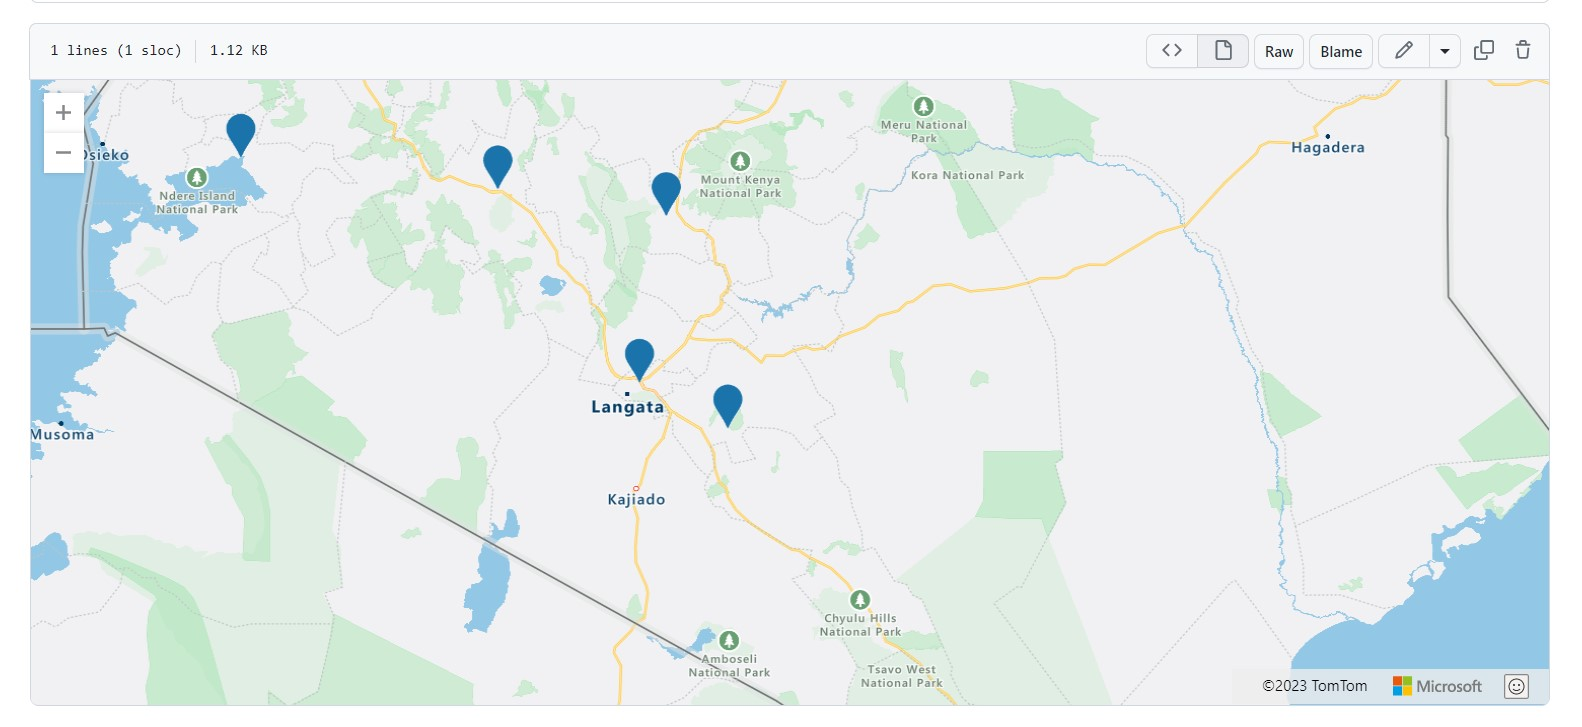
\includegraphics{../images/geojson-webmap.jpg}

However, when the strings are removed, and the population values remain as integers, they are no longer rendered on a webmap as shown below.

\begin{Shaded}
\begin{Highlighting}[]
\NormalTok{knitr}\SpecialCharTok{::}\FunctionTok{include\_graphics}\NormalTok{(}\FunctionTok{rep}\NormalTok{(}\StringTok{"D:/gachuhi/my{-}leaflet/images/geojson{-}nowebmap.jpg"}\NormalTok{))}
\end{Highlighting}
\end{Shaded}

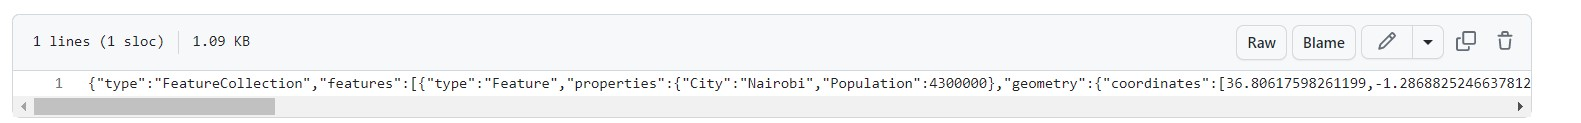
\includegraphics{../images/geojson-nowebmap.jpg}

No map rendered, just a dictionary containing other dictionaries.

\hypertarget{the-icons}{%
\section{The icons}\label{the-icons}}

Alright. Let's create a map of our cities but with custom markers this time round. The below code creates our custom markers.

\begin{verbatim}
// Yellow Icon
var yellowIcon = new L.Icon({
    iconUrl: 'https://raw.githubusercontent.com/pointhi/leaflet-color-markers/master/img/marker-icon-2x-yellow.png',
    shadowUrl: 'https://cdnjs.cloudflare.com/ajax/libs/leaflet/0.7.7/images/marker-shadow.png',
    iconSize: [25, 41],
    iconAnchor: [12, 41],
    popupAnchor: [1, -34],
    shadowSize: [41, 41]
  });

// Orange Icon
var orangeIcon = new L.Icon({
    iconUrl: 'https://raw.githubusercontent.com/pointhi/leaflet-color-markers/master/img/marker-icon-2x-orange.png',
    shadowUrl: 'https://cdnjs.cloudflare.com/ajax/libs/leaflet/0.7.7/images/marker-shadow.png',
    iconSize: [25, 41],
    iconAnchor: [12, 41],
    popupAnchor: [1, -34],
    shadowSize: [41, 41]
  });

// Red Icon
var redIcon = new L.Icon({
    iconUrl: 'https://raw.githubusercontent.com/pointhi/leaflet-color-markers/master/img/marker-icon-2x-red.png',
    shadowUrl: 'https://cdnjs.cloudflare.com/ajax/libs/leaflet/0.7.7/images/marker-shadow.png',
    iconSize: [25, 41],
    iconAnchor: [12, 41],
    popupAnchor: [1, -34],
    shadowSize: [41, 41]
  });
\end{verbatim}

We created three markers in order of importance: yellow, orange, red. You will see the significance (not so much) of these colors later.

Time to create GeoJSON markers out of this.

\begin{verbatim}
L.geoJSON(cities, {
    pointToLayer(feature, latlng) {
        return L.marker(latlng, {icon: yellowIcon});
    }
}).bindPopup(function (layer) {
    return layer.feature.properties.City;
}).addTo(map);
\end{verbatim}

We got this.

\begin{Shaded}
\begin{Highlighting}[]
\NormalTok{knitr}\SpecialCharTok{::}\FunctionTok{include\_graphics}\NormalTok{(}\FunctionTok{rep}\NormalTok{(}\StringTok{"D:/gachuhi/my{-}leaflet/images/geojson{-}markers.jpg"}\NormalTok{))}
\end{Highlighting}
\end{Shaded}

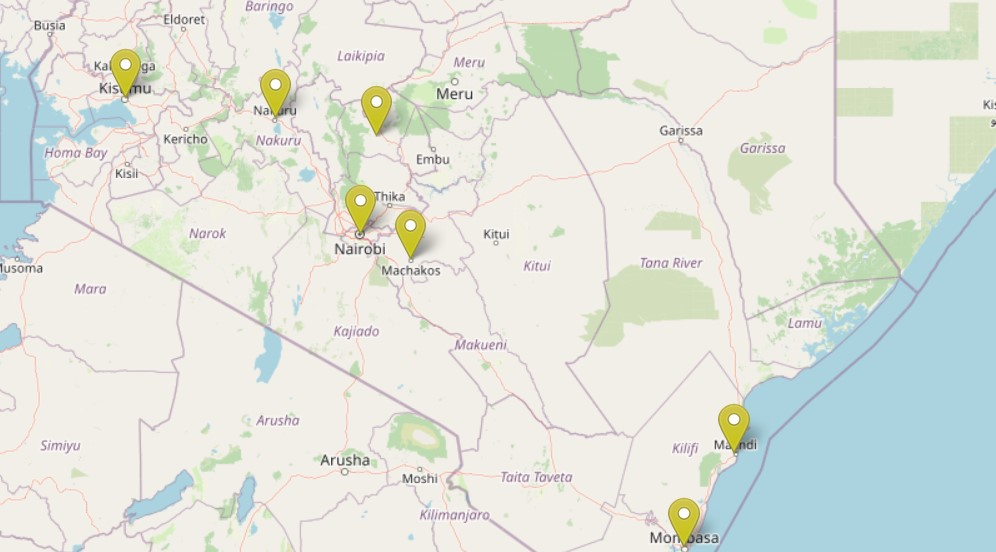
\includegraphics{../images/geojson-markers.jpg}

All cities are marked yellow irrespective of their population or jurisdictional significance. From a cartographer's perspective, the webmap needs more styling but before we get there, what was the purpose of the \texttt{pointToLayer()} function? According to the Leaflet guide, the \texttt{pointToLayer()} function is a special function for GeoJSON variables that specifies how they should be drawn. To be more descriptive, the function parses the \texttt{return\ L.marker...} function to every Lat-Lon coordinate to make a marker appear at that point.

\hypertarget{differentiate-custom-markers-on-a-webmap}{%
\section{Differentiate custom markers on a webmap}\label{differentiate-custom-markers-on-a-webmap}}

Now to the city markers. We would appreciate if the markers would differentiate the cities based on a particular variable, say population. By the way, size of cities is generally determined by population. The below code shall categorize cities by the size of circle markers which shall be based on the city's population. If you've seen point symbols in Qgis, get ready to see them in action in Leaflet!

Comment out the earlier code and insert this:

\begin{verbatim}
L.geoJSON(cities, {
  pointToLayer: function (feature, latlng) {
    if (feature.properties.Population <= 250000) {
      return L.circleMarker(latlng, {
        radius: 4,
        fillColor: '#FFFF00',
        color: '#000',
        weight: 1,
        opacity: 1,
        fillOpacity: 0.8  
      });
    } else if (feature.properties.Population <= 800000) {
      return L.circleMarker(latlng, {
        radius: 8,
        fillColor: '#ff9900',
        color: '#000',
        weight: 1,
        opacity: 1,
        fillOpacity: 0.8  
      });
    } else {
      return L.circleMarker(latlng, {
        radius: 12,
        fillColor: '#FF0000',
        color: '#000',
        weight: 1,
        opacity: 1,
        fillOpacity: 0.8  
      });
    }
    
  }
}).bindPopup(function (layer) {
  return `City: ${layer.feature.properties.City},<br>
  Population: ${layer.feature.properties.Population}`;
}).addTo(map);
\end{verbatim}

What you get is a map where the size of the circle markers has been defined by the city's population. This time round, the \texttt{pointToLayer()} function body worked with \textbf{if/else if} statement to differentiate the radius and color of each circle marker. Under the \textbf{if/else if} code statement block, different circle marker specifications of radius and fillColor were inserted for each population category. Any city with a population beyond 800000 was fitted into the \texttt{else} block.

\begin{Shaded}
\begin{Highlighting}[]
\NormalTok{knitr}\SpecialCharTok{::}\FunctionTok{include\_graphics}\NormalTok{(}\FunctionTok{rep}\NormalTok{(}\StringTok{"D:/gachuhi/my{-}leaflet/images/geojson{-}diff1.jpg"}\NormalTok{))}
\end{Highlighting}
\end{Shaded}

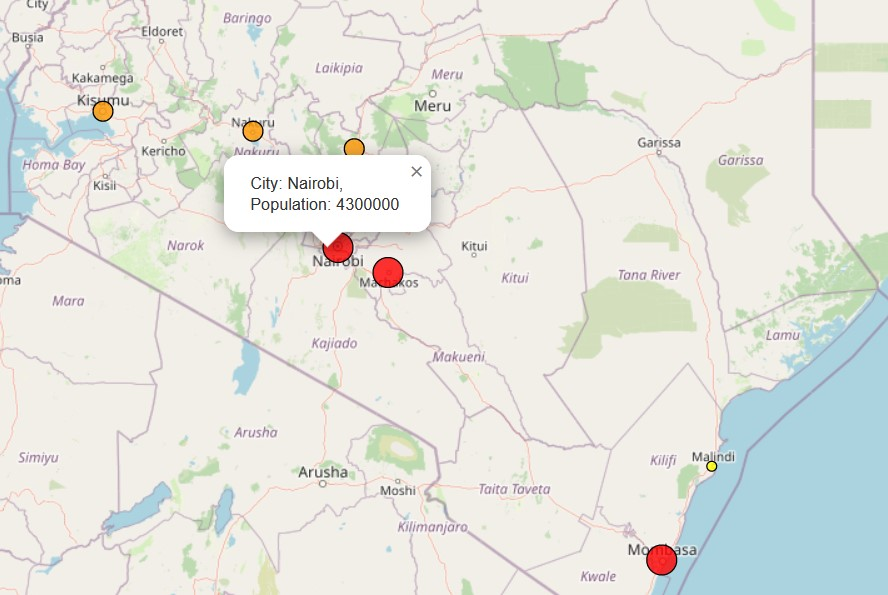
\includegraphics{../images/geojson-diff1.jpg}

This brings us to why we changed the population values from strings to integers. If we were to work with the original string values (like ``1000000'' in quotes), any value beyond 1, 000, 000 would receive the settings of \texttt{feature.properties.Population\ \textless{}=\ 250000}. That is, it would be displayed in the same color scheme of yellow as a city with a population say, 25, 000 people and below. That would be passing a wrong message. The explanation for this glaring error arising from use of string values is this: when ordering numbers enclosed in strings in JavaScript, they will be ordered by their first character irrespective of the size of the value. In other words, 1 is greater than 9 even though the latter is more. Thus a city of \textbf{``\textbf{800, 000}''} people will be treated as bigger than a city of \textbf{``\textbf{1, 000, 000}''}. Now you see the logic of working without the quotes around the \textbf{Population} variable, as is the case with our GeoJSON file.

In the next code sample, we shall create city marker icons whose colors shall be determined by the size of the city's population. We will work with three colors: yellow, orange and red. Yellow shall mark the smallest city while red shall indicate the largest. The below code shows how this categorization is worked out.

\begin{verbatim}
L.geoJSON(cities, {
  pointToLayer: function (feature, latlng) {
    if (feature.properties.Population <= 250000) {
      return L.marker(latlng, {
        icon: yellowIcon 
      });
    } else if (feature.properties.Population <= 800000) {
      return L.marker(latlng, {
        icon: orangeIcon 
      });
    } else {
      return L.marker(latlng, {
        icon: redIcon 
      });
    }
    
  }
}).bindPopup(function (layer) {
  return `City: ${layer.feature.properties.City},<br>
  Population: ${layer.feature.properties.Population}`;
}).addTo(map);
\end{verbatim}

\begin{Shaded}
\begin{Highlighting}[]
\NormalTok{knitr}\SpecialCharTok{::}\FunctionTok{include\_graphics}\NormalTok{(}\FunctionTok{rep}\NormalTok{(}\StringTok{"D:/gachuhi/my{-}leaflet/images/geojson{-}diff2.jpg"}\NormalTok{))}
\end{Highlighting}
\end{Shaded}

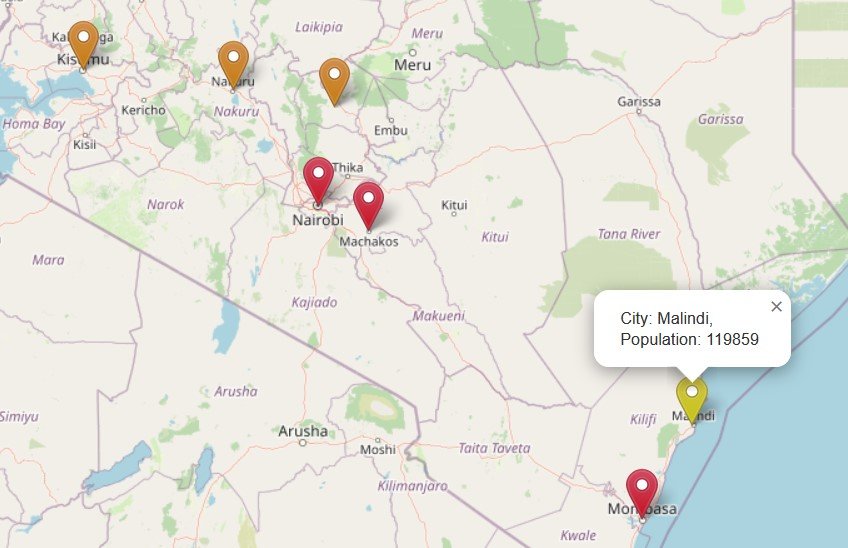
\includegraphics{../images/geojson-diff2.jpg}

In the above map, large cities with populations above 800, 000 have been categorized with a red marker, those with populations below 250, 000 with a yellow marker and those in between with an orange marker. In all cases, our \texttt{bindPopup()} still contains the same settings of showing both the city name and population size.

The value to the \texttt{pointToLayer()} key was assigned a function that checks if a city's population is within a specific range. If a city falls within the range specified by the \texttt{if} statement, a particular icon --whether \texttt{yellowIcon}, \texttt{orangeIcon} or \texttt{redIcon} is returned by the \texttt{L.marker()} function.

\hypertarget{using-fetch}{%
\section{Using fetch}\label{using-fetch}}

Remember how \texttt{fetch} helped us retrieve data from a server in a previous chapter? Whereas we won't repeat the entire process again (you can breathe a sigh of relief), the same iterations of differentiating a marker icon can also be inserted into the \texttt{fetch} API. All this is done right within the options of \texttt{L.geoJson(data,\ \{options\})}.

\begin{verbatim}
fetch("https://raw.githubusercontent.com/sammigachuhi/geojson_files/main/cities-geojson2.geojson.txt")
    .then((response) =>{
        return response.json()
    })
    .then((data) => {
        L.geoJson(data, {
          pointToLayer: function (feature, latlng) {
            if (feature.properties.Population <= 250000) {
              return L.marker(latlng, {
                icon: yellowIcon 
              });
            } else if (feature.properties.Population <= 800000) {
              return L.marker(latlng, {
                icon: orangeIcon 
              });
            } else {
              return L.marker(latlng, {
                icon: redIcon 
              });
            }
            
          }
        }).bindPopup((layer) => {
            return `City: ${layer.feature.properties.City},<br>
            Population: ${layer.feature.properties.Population}`}).addTo(map);
    })
    .catch((error) => {
        console.log(`This is the error: ${error}`)
    })
\end{verbatim}

The resulting map should look like the previous one.

\begin{Shaded}
\begin{Highlighting}[]
\NormalTok{knitr}\SpecialCharTok{::}\FunctionTok{include\_graphics}\NormalTok{(}\FunctionTok{rep}\NormalTok{(}\StringTok{"D:/gachuhi/my{-}leaflet/images/cities\_colored.jpg"}\NormalTok{))}
\end{Highlighting}
\end{Shaded}

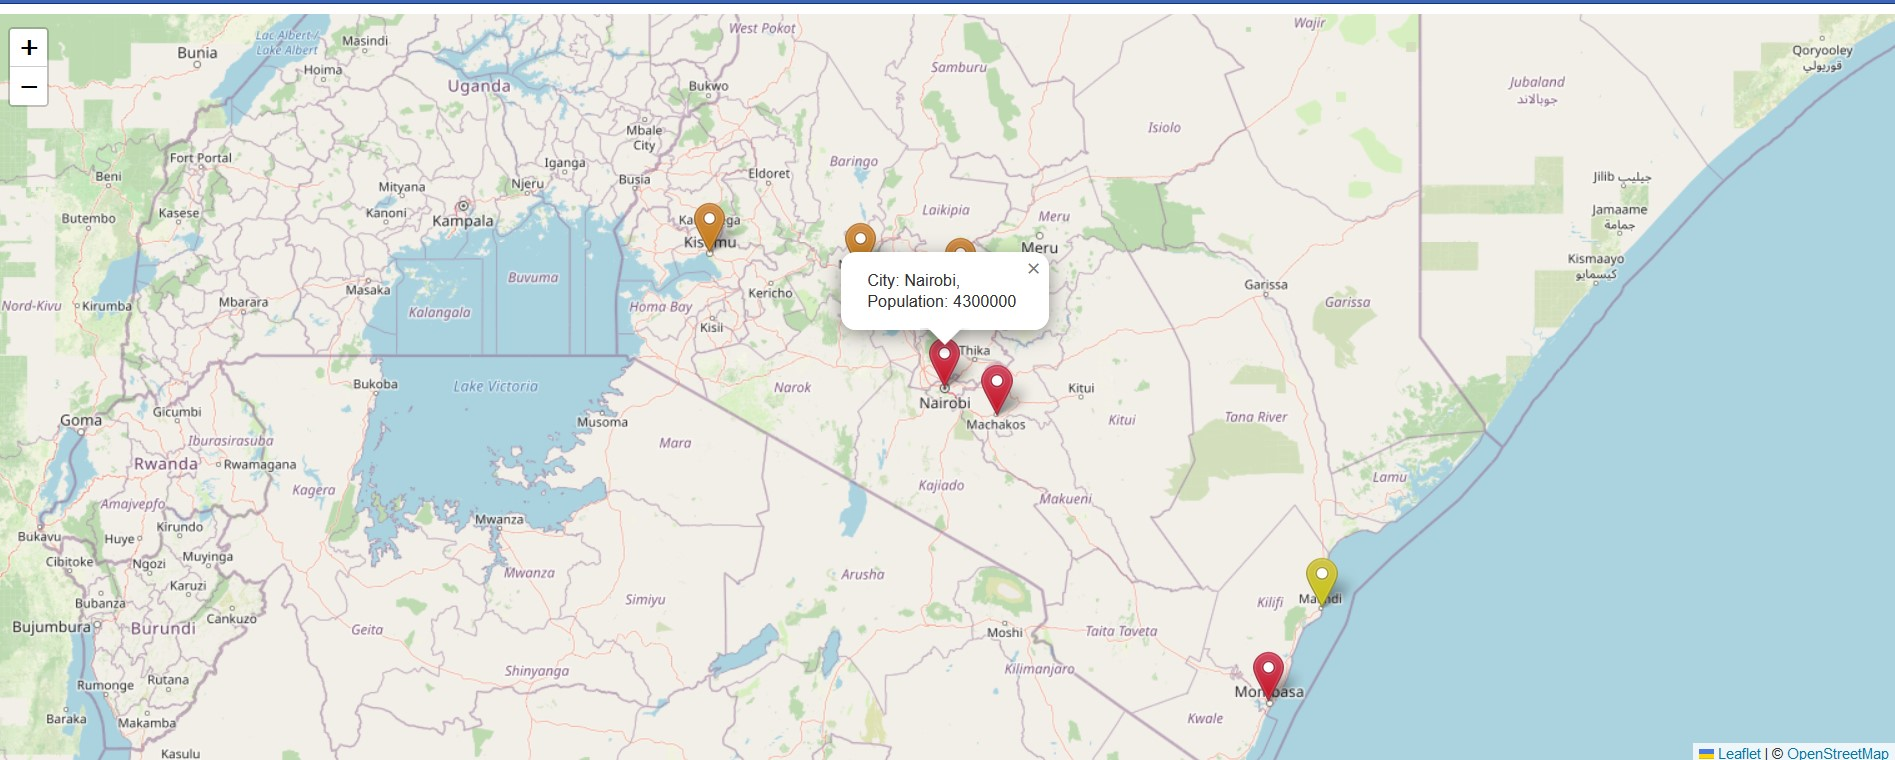
\includegraphics{../images/cities_colored.jpg}

\hypertarget{unique-custom-markers}{%
\section{Unique custom markers}\label{unique-custom-markers}}

This part may not be necessary, but it has been inserted to show you that there are various markers apart from the defaults provided by Leaflet. One can create custom markers outside of Leaflet using the \href{https://github.com/lennardv2/Leaflet.awesome-markers}{Leaflet.Awesome.Markers plugin}. Just like in the case of Ajax, you will need to provide the path to the plugin's dependencies using the \texttt{\textless{}script\textgreater{}} tag. Insert the following \texttt{\textless{}script\textgreater{}} tags into \texttt{map.html}.

\begin{verbatim}
<script src="Leaflet.awesome-markers-2.0-develop\Leaflet.awesome-markers-2.0-develop\dist\leaflet.awesome-markers.js"></script>

<script src="Leaflet.awesome-markers-2.0-develop\Leaflet.awesome-markers-2.0-develop\dist\leaflet.awesome-markers.css"></script>
\end{verbatim}

And also this \texttt{\textless{}link\textgreater{}} tag:

\begin{verbatim}
<link href="http://netdna.bootstrapcdn.com/font-awesome/4.0.0/css/font-awesome.css" rel="stylesheet"> 
\end{verbatim}

To make the best use of time, following the example on their site, we simply replace the value of our \texttt{icon} keys with the new \texttt{L.AwesomeMarkers.icon}. We also tweaked the colors for each icon to match those used previously. Because these markers signify various amenities, we made some overly simplified assumptions for the sake of demonstrating their use ie. big cities with a population above 1, 000, 000 have the best malls, those with a population between 250, 000 and 800, 000 must be having good coffee places, and those with populations below 250, 000 obviously have respectable industries. We assume fair play has been exercised in our assumptions. So here is the code.

\begin{verbatim}
L.geoJSON(cities, {
    pointToLayer: function (feature, latlng) {
      if (feature.properties.Population <= 250000) {
        return L.marker(latlng, {
          icon: L.AwesomeMarkers.icon({icon: 'cog', prefix: 'fa', markerColor: 'purple', iconColor: 'yellow'}) 
        });
      } else if (feature.properties.Population <= 800000) {
        return L.marker(latlng, {
          icon: L.AwesomeMarkers.icon({icon: 'coffee', prefix: 'fa', markerColor: 'red', iconColor: 'orange'}) 
        });
      } else {
        return L.marker(latlng, {
          icon: L.AwesomeMarkers.icon({icon: 'shopping-cart', prefix: 'fa', markerColor: 'blue', iconColor: 'red'})
        });
      }
      
    }
  }).bindPopup(function (layer) {
    return `City: ${layer.feature.properties.City},<br>
    Population: ${layer.feature.properties.Population}`;
  }).addTo(map);
\end{verbatim}

\begin{Shaded}
\begin{Highlighting}[]
\NormalTok{knitr}\SpecialCharTok{::}\FunctionTok{include\_graphics}\NormalTok{(}\FunctionTok{rep}\NormalTok{(}\StringTok{"D:/gachuhi/my{-}leaflet/images/extra{-}markers.jpg"}\NormalTok{))}
\end{Highlighting}
\end{Shaded}

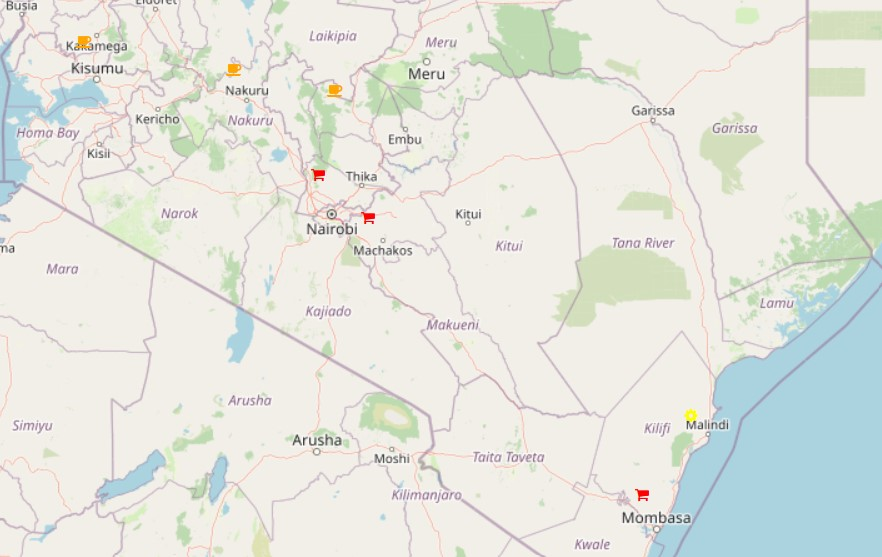
\includegraphics{../images/extra-markers.jpg}

The custom markers are also clickable!

\hypertarget{image-overlays}{%
\section{Image overlays}\label{image-overlays}}

Sometimes an image can act as good a marker. Overlaying images on a map is fairly easy. The below code inserts an image above a historical monument located in the Kenyan capital, Nairobi.

\begin{verbatim}
// Image overlays
var imageUrl = 'https://pbs.twimg.com/media/DddQBk5WsAAlbdJ?format=jpg&name=large';
var errorOverlayUrl = 'https://pbs.twimg.com/media/DddQBk5WsAAlbdJ?format=jpg&name=large';
var altText = 'The Galton - Fenzi Memorial: Source: Google and Twitter';
var latLngBounds = L.latLngBounds([[-1.2861259,36.8172709], [-1.2886193,36.8230413]]);

var imageOverlay = L.imageOverlay(imageUrl, latLngBounds, {
    opacity: 0.8,
    errorOverlayUrl: errorOverlayUrl,
    alt: altText,
    interactive: true
}).addTo(map);

\end{verbatim}

However, finding an image of just one location over the wide earth can be laborious, so we envelope it with a rectangle. The \texttt{map.fitBounds} function enables the browser to automatically zoom to where our image is placed.

\begin{verbatim}
L.rectangle(latLngBounds).addTo(map);
map.fitBounds(latLngBounds);
\end{verbatim}

\begin{Shaded}
\begin{Highlighting}[]
\NormalTok{knitr}\SpecialCharTok{::}\FunctionTok{include\_graphics}\NormalTok{(}\FunctionTok{rep}\NormalTok{(}\StringTok{"D:/gachuhi/my{-}leaflet/images/geltan{-}fenzi.jpg"}\NormalTok{))}
\end{Highlighting}
\end{Shaded}

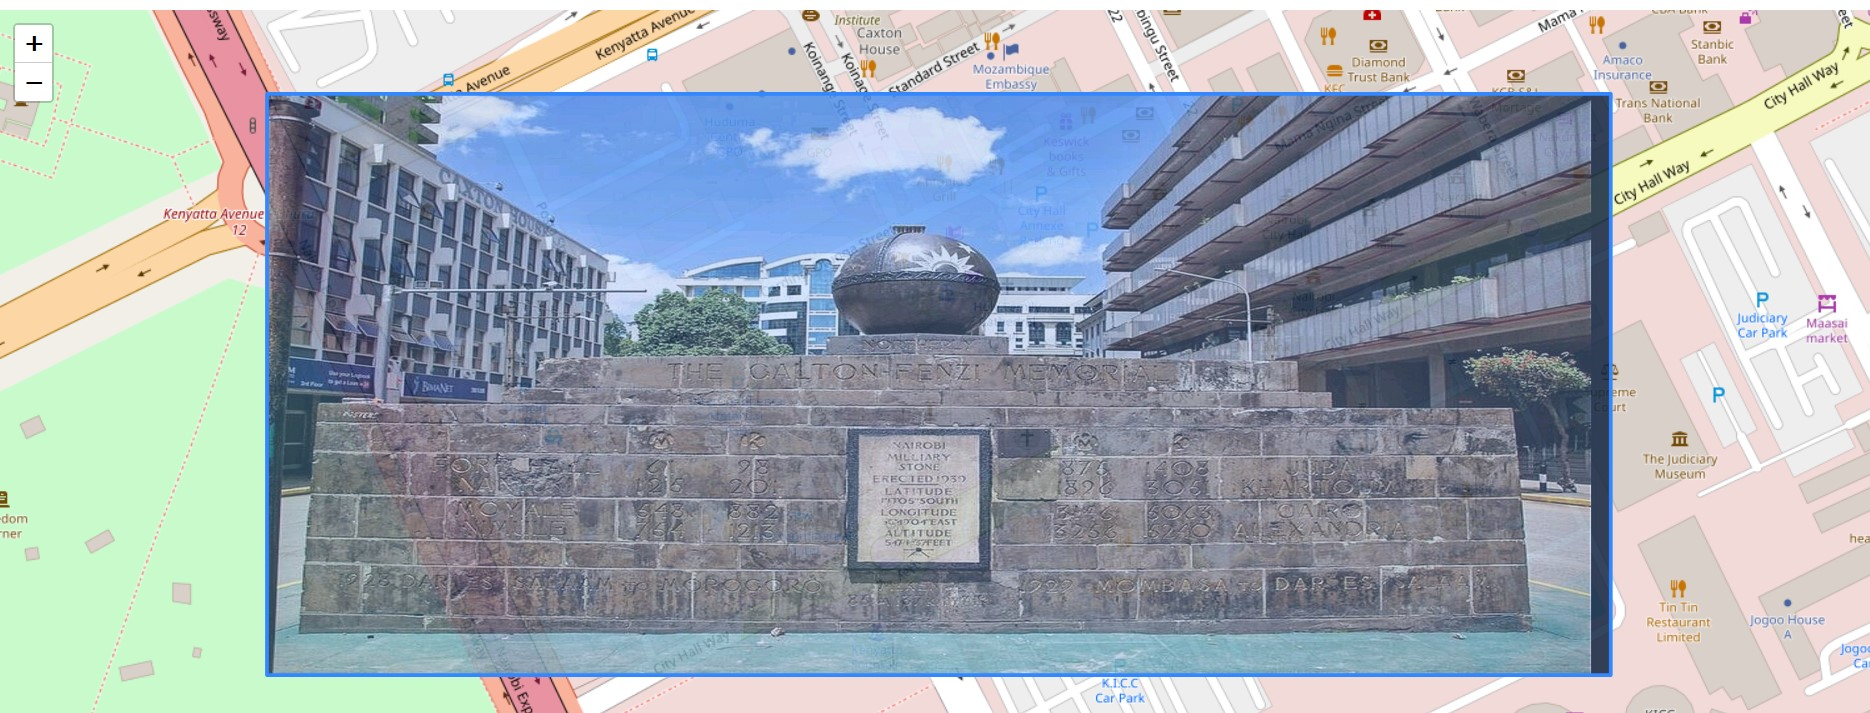
\includegraphics{../images/geltan-fenzi.jpg}

Mind you that landmark was set up in 1939 in honour of Lionel Douglas Galton-Fenzi; the first motorist to drive from Nairobi to Mombasa as early as 1926. The landmark is also inscribed with bearings to various East African cities but enough history for today.

Anyway, here is a quick breakdown of the attributes used in \texttt{L.imageOverlay}: a) the \texttt{var\ latLngBounds} uses the \texttt{L.latLngBounds} class to set the lat-lon coordinates. Notice they are two coordinate lists bound with a single \texttt{{[}{]}}. Failing to enclose the two coordinates with \texttt{{[}{]}} results in an error. b) \texttt{var\ ImageUrl} is the image source.

For the additional options parsed to the \texttt{L.imageOverlay()} class, they are described below:

\begin{enumerate}
\def\labelenumi{\arabic{enumi}.}
\item
  \texttt{opacity} - defines the opacity of the image overlay, it equals to 1.0 by default. Decrease this value to make an image overlay transparent and to expose the underlying map layer.
\item
  \texttt{errorOverlayUrl} - is a URL to the overlay image to show in place of the overlay that failed to load.
\item
  \texttt{alt} - sets the HTML alt attribute to provide an alternative text description of the image. It is quite helpful in describing an image in text form just in case it fails to load due to poor network connectivity. Moreover, it can improve the Search Engine Optimization (SEO) of the website it is hosted in.
\item
  \texttt{interactive} - is false by default. If true, the image overlay will emit mouse events when clicked or hovered.
\end{enumerate}

Full codes and files are \href{https://github.com/sammigachuhi/my-leaflet-project/tree/main/my-leaflet-code/chapter-6-custom-markers}{here}.

\hypertarget{summary-5}{%
\section{Summary}\label{summary-5}}

This was quite a long chapter that rendered justice on how to customize GeoJSON markers in Leaflet. Through the various exercises you encountered in this chapter, you have learnt the following:

\begin{itemize}
\item
  GeoJSON files, if in the correct format, can be rendered as a standalone map from Github. An example is \href{https://github.com/sammigachuhi/geojson_files/blob/main/cities-geojson.geojson}{here}.
\item
  One can customize marker colour or size based on the GeoJSON's file attributes. In this chapter, the city population values were used to define the marker's size and colour.
\item
  The \texttt{pointToLayer} key, when used as an option in \texttt{L.geoJSON}, will parse a particular function to every Lat-Lon coordinate of the GeoJSON object.
\item
  It is also possible to customize markers in the \texttt{fetch} API by simply specifying how they should appear, in form of functions, within the \texttt{L.geoJson} options environment.
\item
  There exist plenty of custom made icons outside of, but compatible with Leaflet. An example of such a library is \href{https://github.com/lennardv2/Leaflet.awesome-markers}{Leaflet Awesome Markers}.
\item
  Images can also be overlayed on a Leaflet map. This was done in the sub-chapter of \protect\hyperlink{image-overlays}{Image Overlays}.
\end{itemize}

\hypertarget{creating-an-interactive-choropleth-map}{%
\chapter{Creating an interactive choropleth map}\label{creating-an-interactive-choropleth-map}}

\hypertarget{what-is-a-choropleth-map}{%
\section{What is a choropleth map?}\label{what-is-a-choropleth-map}}

We will now move from markers to something larger than life --choropleth maps. \emph{What the heck are choropleth maps?} You may ask. Geographers will roll their eyes over this term because they have come across it innumerable times throughout their career. However, for the sake of new readers, a \href{https://datavizcatalogue.com/methods/choropleth.html}{choropleth map} is a map whose geographical areas or regions are colored, shaded or patterned in relation to a data variable. If during election time you have seen a map that has draped the winning candidate in (a) particular state(s) with their party theme colors, then that's a choropleth map. Most population maps are also choropleth maps. In this chapter, we will create a choropleth map of Kenyan counties, and make it interactive by leveraging the area and population characteristics of each county.

\begin{Shaded}
\begin{Highlighting}[]
\NormalTok{knitr}\SpecialCharTok{::}\FunctionTok{include\_graphics}\NormalTok{(}\FunctionTok{rep}\NormalTok{(}\StringTok{"D:/gachuhi/my{-}leaflet/images/choropleth.png"}\NormalTok{))}
\end{Highlighting}
\end{Shaded}

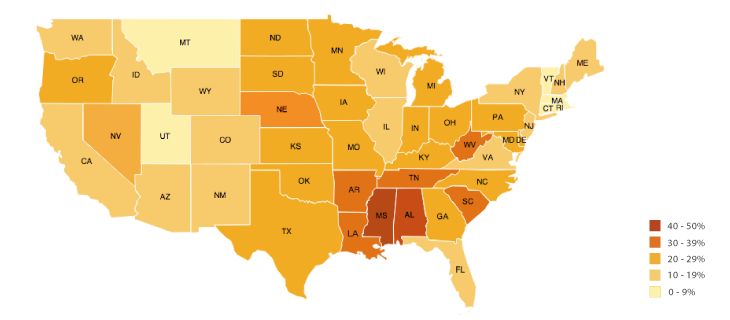
\includegraphics[width=10.14in]{../images/choropleth}

Source: \href{https://www.google.com/url?sa=i\&url=https\%3A\%2F\%2Fdatavizcatalogue.com\%2Fmethods\%2Fchoropleth.html\&psig=AOvVaw2doHr7xcU75mGuozmp6T5M\&ust=1689793060222000\&source=images\&cd=vfe\&opi=89978449\&ved=0CBMQjhxqFwoTCJiIu-v3mIADFQAAAAAdAAAAABAE}{The Data Visualization Catalogue}

\hypertarget{creating-a-choropleth-map-the-start}{%
\section{Creating a choropleth map: the start}\label{creating-a-choropleth-map-the-start}}

Obviously by now, without going into much details, you can now create a basic Leaflet map blindfolded. Anyway, seeing is believing, so lets start it right away anyway. Create another new JavaScript file called \texttt{interactive-choropleth.js}. To break the monotony, we shall use a different tile layer. Remember that Leaflet has several \href{https://leaflet-extras.github.io/leaflet-providers/preview/}{tile layer servers}, and CyclOSM, used in this chapter is just one among many.

\begin{verbatim}
var map = L.map('myMap').setView([0.3556, 37.5833], 6.5);

L.tileLayer('https://{s}.tile-cyclosm.openstreetmap.fr/cyclosm/{z}/{x}/{y}.png', {
    maxZoom: 20,
    attribution: '<a href="https://github.com/cyclosm/cyclosm-cartocss-style/releases" title="CyclOSM - Open Bicycle render">CyclOSM</a> | Map data: &copy; <a href="https://www.openstreetmap.org/copyright">OpenStreetMap</a> contributors'
}).addTo(map); // the CyclOSM tile layer available from Leaflet servers
\end{verbatim}

Now to the big part --the GeoJSON files. We would like to mention it was quite a hustle to set up the GeoJSON file to be in a format accessible by JavaScript's Fetch API. Only when we converted the GeoJSON to \texttt{.json} were we able to successfully view it using \texttt{fetch}. The raw json file for our Kenyan counties which we shall use in creating a choropleth map is available from \href{https://raw.githubusercontent.com/sammigachuhi/geojson_files/main/counties_json.json}{here} or \href{https://raw.githubusercontent.com/sammigachuhi/my-leaflet-project/main/geojson_files_updated/counties_json.json}{here}.

Let's fetch the counties json file.

\begin{verbatim}
fetch("https://raw.githubusercontent.com/sammigachuhi/geojson_files/main/counties_json.json")
    .then((response) =>{
        return response.json()
    })
    .then((data) => {
        L.geoJson(data, {style: style}).addTo(map);
    })
    .catch((error) => {
        console.log(`This is the error: ${error}`)
    })
    
\end{verbatim}

So far, you should get a result like below.

\begin{Shaded}
\begin{Highlighting}[]
\NormalTok{knitr}\SpecialCharTok{::}\FunctionTok{include\_graphics}\NormalTok{(}\FunctionTok{rep}\NormalTok{(}\StringTok{"D:/gachuhi/my{-}leaflet/images/kenya\_json.jpg"}\NormalTok{))}
\end{Highlighting}
\end{Shaded}

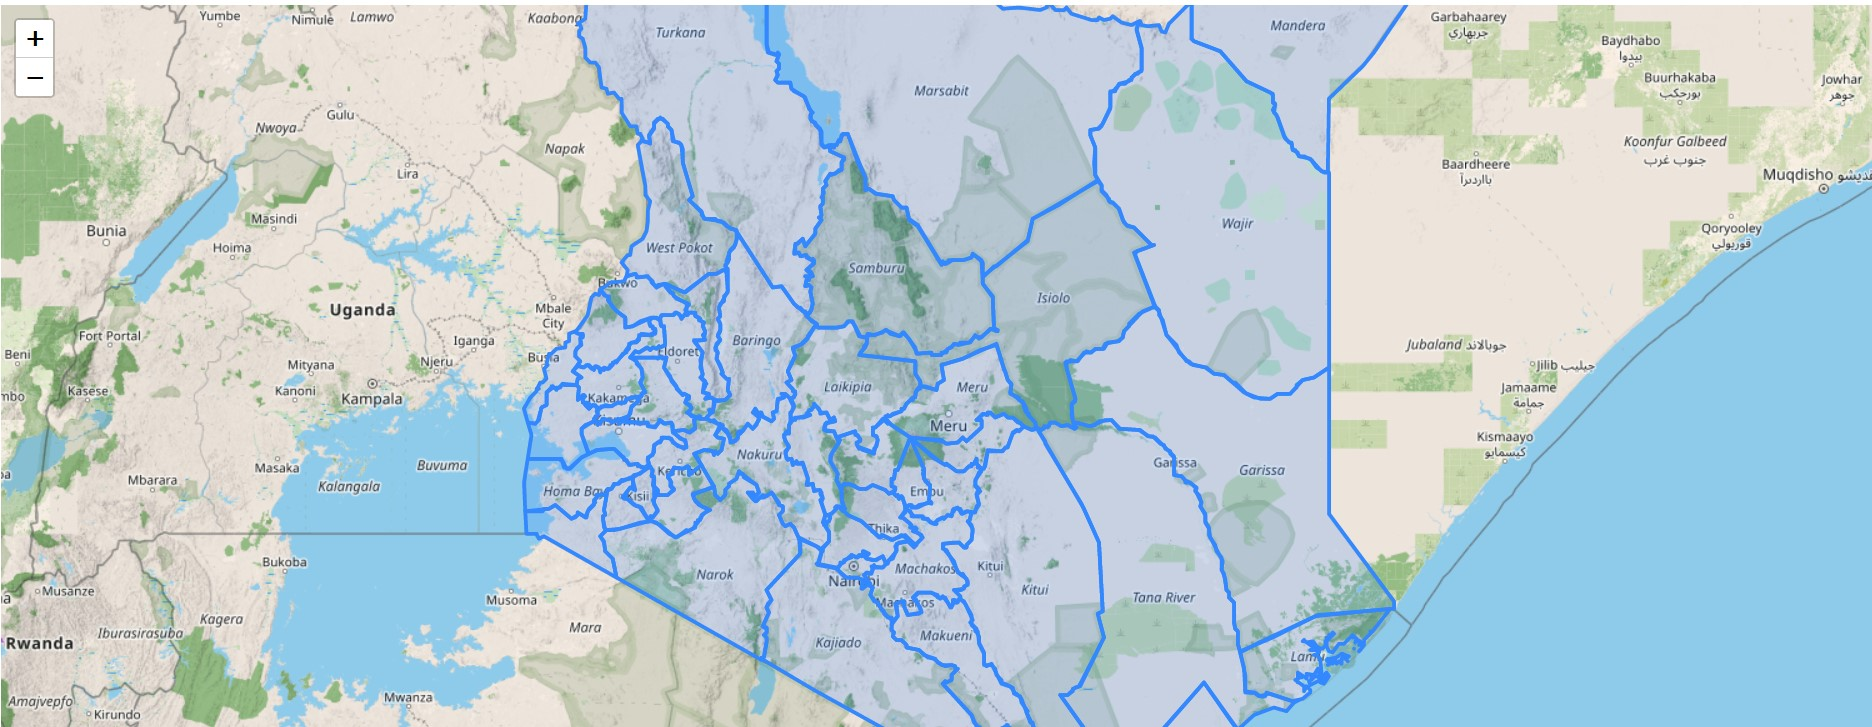
\includegraphics{../images/kenya_json.jpg}

\hypertarget{coloring-the-counties}{%
\section{Coloring the counties}\label{coloring-the-counties}}

Alright, we have been able to load our json file to a Leaflet map. However, it looks dull and provides no meaningful information to the casual observer. When making maps, aim to provide information at lightning speed. That is, inform the reader at first glance. The code snippets that follow have been heavily borrowed from Volodymyr's interactive \href{https://leafletjs.com/examples/choropleth/}{choropleth tutorial}.

First, let's create a function that sets a hex colour code for each population category. We used \href{https://colorbrewer2.org/\#type=sequential\&scheme=BuGn\&n=3}{color brewer} for this.

Take a look at this code and we shall explain.

\begin{verbatim}
//// Adding some color
function getColor(d) {
    return d > 1400 ? '#8c2d04' :
            d > 700 ? '#cc4c02' :
            d > 400 ? '#ec7014' :
            d > 100 ? '#fe9929' :
            d >  50 ?  '#fec44f':
            d > 25 ?   '#fee391':
                       '#ffffd4';
}
\end{verbatim}

The above function uses a question mark \texttt{?} to act as the \texttt{if...else} statement. In JavaScript, this is known as a \href{https://www.freecodecamp.org/news/how-the-question-mark-works-in-javascript/}{ternary operator}. A ternary operator? What's that? How does it work?

For a ternary operator, any statement to the right of the \texttt{?} is returned as true if it agrees with the value to the left of the \texttt{?}. Reread that last statement. If the value to the right of the \texttt{?} is false, then the value after the colon \texttt{:} is returned. Reread that last statement for this ternary operator concept to sink in.

If it still sounds fuzzy, the below image adapted from \href{https://www.freecodecamp.org/news/how-the-question-mark-works-in-javascript/}{FreeCodeCamp} should help.

\begin{Shaded}
\begin{Highlighting}[]
\NormalTok{knitr}\SpecialCharTok{::}\FunctionTok{include\_graphics}\NormalTok{(}\FunctionTok{rep}\NormalTok{(}\StringTok{"D:/gachuhi/my{-}leaflet/images/ternary.png"}\NormalTok{))}
\end{Highlighting}
\end{Shaded}

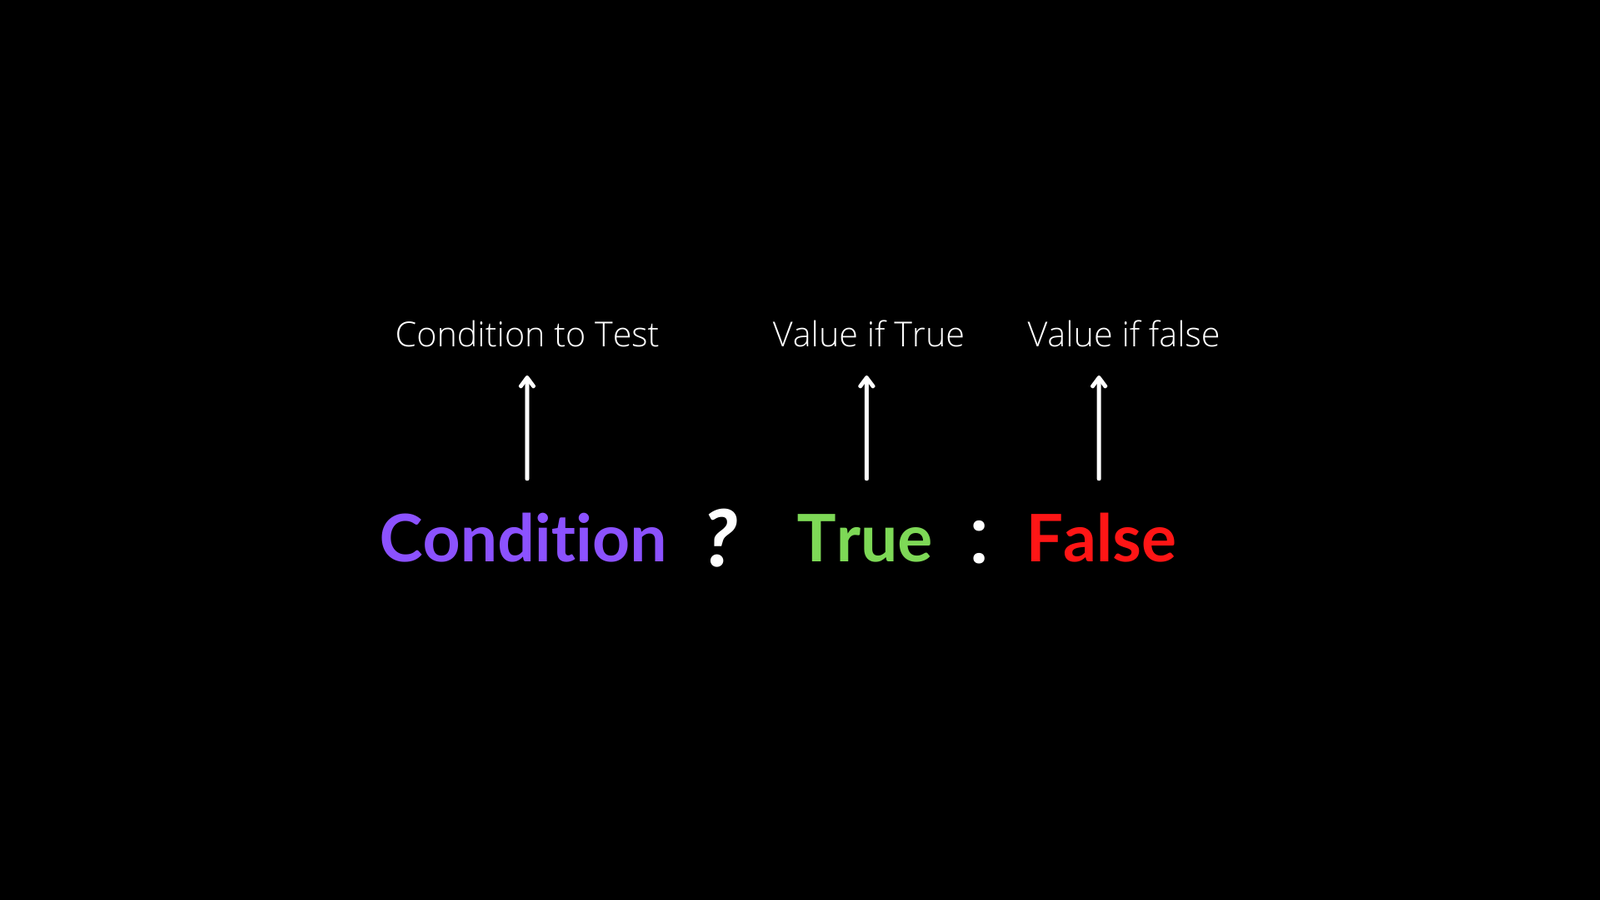
\includegraphics[width=22.22in]{../images/ternary}

In other words, the ternary operator is a short form of writing the \texttt{if...else} statement over several lines. Look at the below code which is simply the \texttt{if...else} version of the ternary operator we've used above. Definitely, the ternary operator wins the day in terms of brevity.

\begin{verbatim}
function getColor(d) {
  if (d > 1400) {
    return '#8c2d04';
  } else if (d > 700) {
    return '#cc4c02';
  } else if (d > 400) {
    return '#ec7014';
  } else if (d > 100) {
    return '#fe9929';
  } else if (d > 50) {
    return '#fec44f';
  } else if (d > 25) {
    return '#fee391';
  } else {
    return '#ffffd4';
  }
}
\end{verbatim}

Now that we've created the function of setting colors to our json file on Leaflet, we next also have to \emph{create} a function that applies the color designation to the counties in the GeoJSON file itself. Luckily, we have the \textbf{style} \href{https://leafletjs.com/reference.html\#geojson-style}{option from Leaflet} which is a function for precisely styling GeoJSON lines and polygons alone. We saw it in \protect\hyperlink{using-geojson-in-leaflet}{Chapter 5} and we shall also use it here.

\begin{verbatim}
var style = ((feature)=> {
    return {
        fillColor: getColor(feature.properties.Pop_Density),
        weight: 2,
        opacity: 1,
        color: 'gray',
        fillOpacity: 0.5
    }
})
\end{verbatim}

The above is an arrow function. Unlike regular JavaScript function declarations which are in the format of \texttt{function\ \textless{}name\ of\ function\textgreater{}\ (\textless{}parameter\textgreater{})}, we remove the \texttt{function} keyword, enclose everything in brackets and put an arrow \texttt{=\textgreater{}} between the parameter brackets and function body. That's just it. Arrow functions aren't so hard!

Remember we assign the arrow function to a variable called \texttt{var\ style} since we will parse it to the \texttt{L.geoJson} class.

Finally, we add the \texttt{style} variable to the \textbf{style} option of \texttt{L.geoJson} class.

\begin{verbatim}
fetch("https://raw.githubusercontent.com/sammigachuhi/geojson_files/main/counties_json.json")
    .then((response) =>{
        return response.json()
    })
    .then((data) => {
        L.geoJson(data, {style: style}).addTo(map);
    })
    .catch((error) => {
        console.log(`This is the error: ${error}`)
    })
    
\end{verbatim}

Since the \textbf{style} option is a key (and also a function), the value will be the \texttt{var\ style} which we created. This value is in and by itself a function that iterates over every county because of the \texttt{getColor(feature.properties.Pop\_Density)} contained in it as the \texttt{fillColor} value!

Enough JavaScript for one day!

\begin{Shaded}
\begin{Highlighting}[]
\NormalTok{knitr}\SpecialCharTok{::}\FunctionTok{include\_graphics}\NormalTok{(}\FunctionTok{rep}\NormalTok{(}\StringTok{"D:/gachuhi/my{-}leaflet/images/choropleth{-}map.jpg"}\NormalTok{))}
\end{Highlighting}
\end{Shaded}

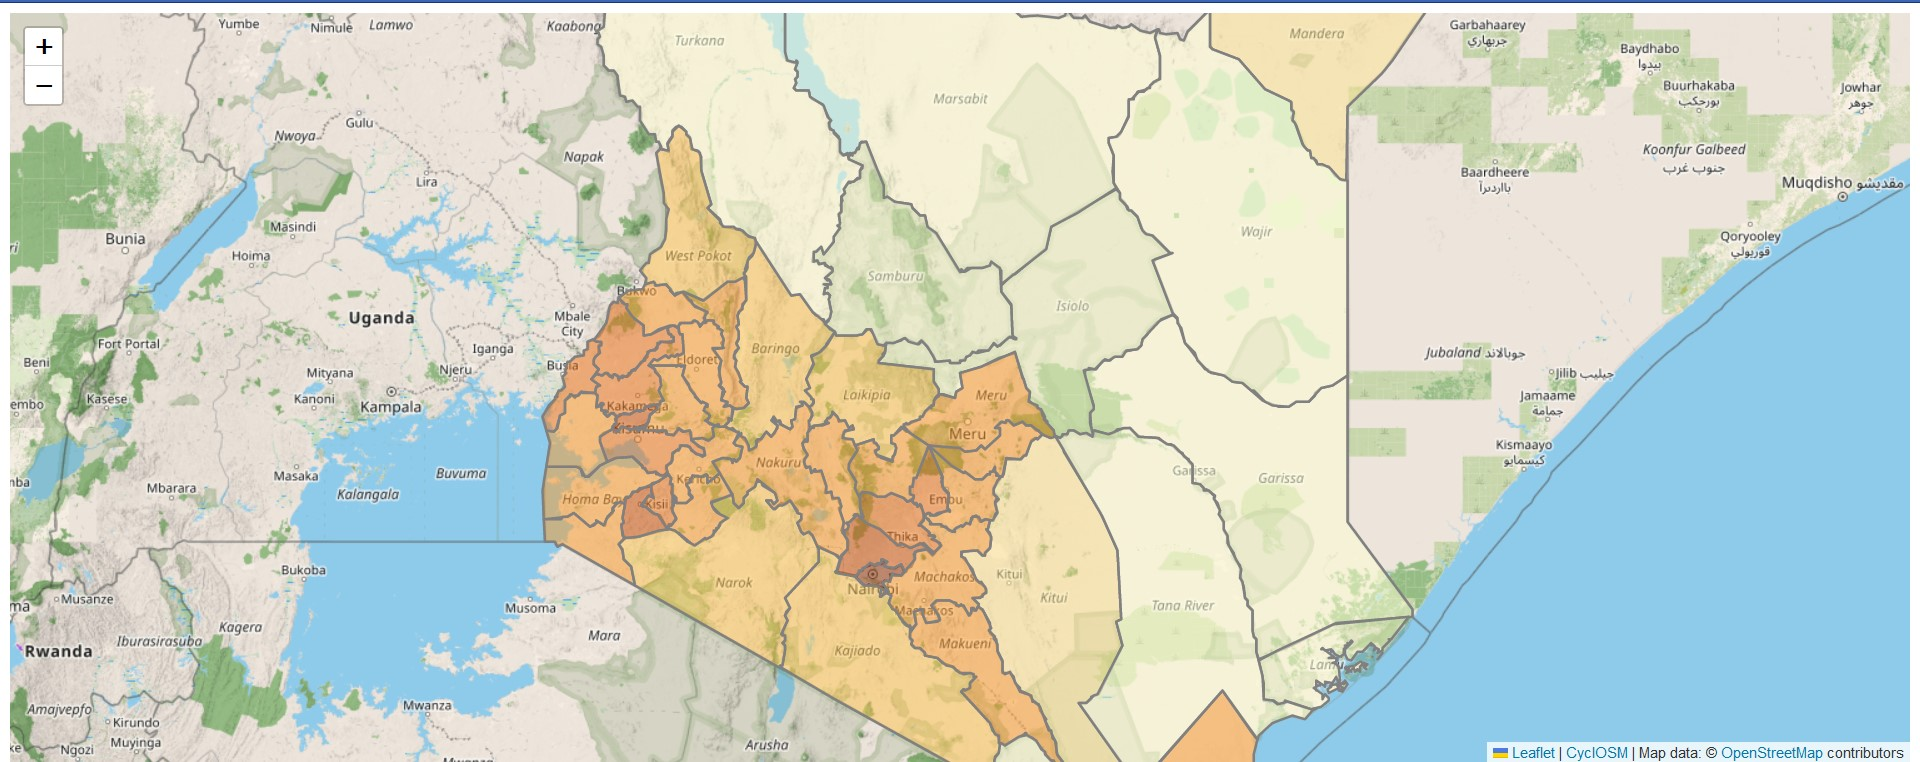
\includegraphics{../images/choropleth-map.jpg}

Our choropleth map is beginning to take shape.

\hypertarget{highlight-features}{%
\section{Highlight features}\label{highlight-features}}

Going on from where we last left, we would like the choropleth map to highlight any county that the screen pointer (or mouse) hovers over. Additionally, upon clicking, the map should zoom to the clicked county as well as display its attributes. The counties should also be reset to their default characteristics when the screen pointer hovers out.

Alright. It seems like we have our hands full.

Let's start simple, and scale upwards in terms of complexity.

Remember the \texttt{fetch} API we had used in retrieving our json file? We will tweak it a bit by adding the \texttt{var\ geojson} just before calling the \texttt{L.geoJson} class. We shall parse the variable \texttt{var\ geojson} to the \texttt{L.geoJson} class. We shall explain why we are assigning \texttt{L.geoJson} to a variable (\texttt{var\ geojson}) when we know very well it can work alone, as seen in the last two previous chapters.

\begin{verbatim}
fetch("https://raw.githubusercontent.com/sammigachuhi/geojson_files/main/counties_json.json")
    .then((response) =>{
        return response.json()
    })
    .then((data) => {
        var geojson;
        geojson = L.geoJson(data, {
            style: style,
            --snip--
    })
\end{verbatim}

We had initially mentioned that we wanted the county hovered over to be highlighted. The following code will highlight with a white hue the county hovered over while also seemingly popping it out above the rest.

\begin{verbatim}

        geojson = L.geoJson(data, {
            style: style,
            onEachFeature: ((feature, layer) => {
                layer.on('mouseover', ((e) => {
                    var layer = e.target;
                
                    layer.setStyle({
                        weight: 5,
                        color: '#FFFFFF',
                        dashArray: '',
                        fillOpacity: 0.7
                    });
                
                    layer.bringToFront();
                }))
                
                
\end{verbatim}

The purpose of \texttt{on} method is to add an event listener. Event listeners in JavaScript are functions that run a code when the browser user interacts with the browser in a specific way. Now what \texttt{on} method does is that it triggers the event listener \texttt{mouseover} for each county in our GeoJSON layer. The \texttt{mouseover} event is what makes our counties be highlighted and `pop' out when a screen pointer is \emph{over} them.

Since the change in state of an element in HTML is known as an event (denoted as \texttt{e} in our case), the \texttt{e.target} property returns the element on which the event is occurring on. Since it's a particular county in our case, we proceed to change its symbology through the parameters in the \texttt{setStyle} function. Thereafter we use the \texttt{bringToFront} method to make the element in which the event has happened on to `pop' out above the rest.

Remember we had mentioned we also want the counties to be reset to their default status when one hovers out to some other county or outside the map altogether. The following code does the job.

\begin{verbatim}
layer.on('mouseout', function() {
                    geojson.resetStyle(this);
                })
\end{verbatim}

We use the \texttt{resetStyle} function to return the layer to default settings but there is a twist. In the \texttt{resetStyle} case, we add the argument \texttt{this} in parenthesis to refer to the element that was received. In other words, when the mouse `hovers out' of a county, the element will revert to its original symbology.

Before, we end this monologue, we ensure we pass the variable \texttt{geojson} to \texttt{resetStyle} function or else it won't work. This appears to be the \emph{modus operandi} for resetting styles in Leaflet as shown in this \href{https://stackoverflow.com/questions/35072630/why-doesnt-resetstyle-of-leaflet-work-for-me}{Stack Overflow question} and also \href{https://stackoverflow.com/questions/21029533/reset-style-on-leaflet-polygon-on-click}{here}.

Finally, we mentioned we want to zoom to a particular county upon clicking it. The following code fits our map to the bounds of the particular county that was clicked. Note that \texttt{fitBounds} is parsed \texttt{getBounds} which gets the boundaries of the county clicked upon. The browser is able to identify the county clicked upon through the help of the \texttt{e} parameter and \texttt{e.target}.

\begin{verbatim}
layer.on('click', ((e) => {
                    map.fitBounds(e.target.getBounds())
                }))
\end{verbatim}

\begin{Shaded}
\begin{Highlighting}[]
\NormalTok{knitr}\SpecialCharTok{::}\FunctionTok{include\_graphics}\NormalTok{(}\FunctionTok{rep}\NormalTok{(}\StringTok{\textquotesingle{}D:/gachuhi/my{-}leaflet/images/highlightable{-}map.jpg\textquotesingle{}}\NormalTok{))}
\end{Highlighting}
\end{Shaded}

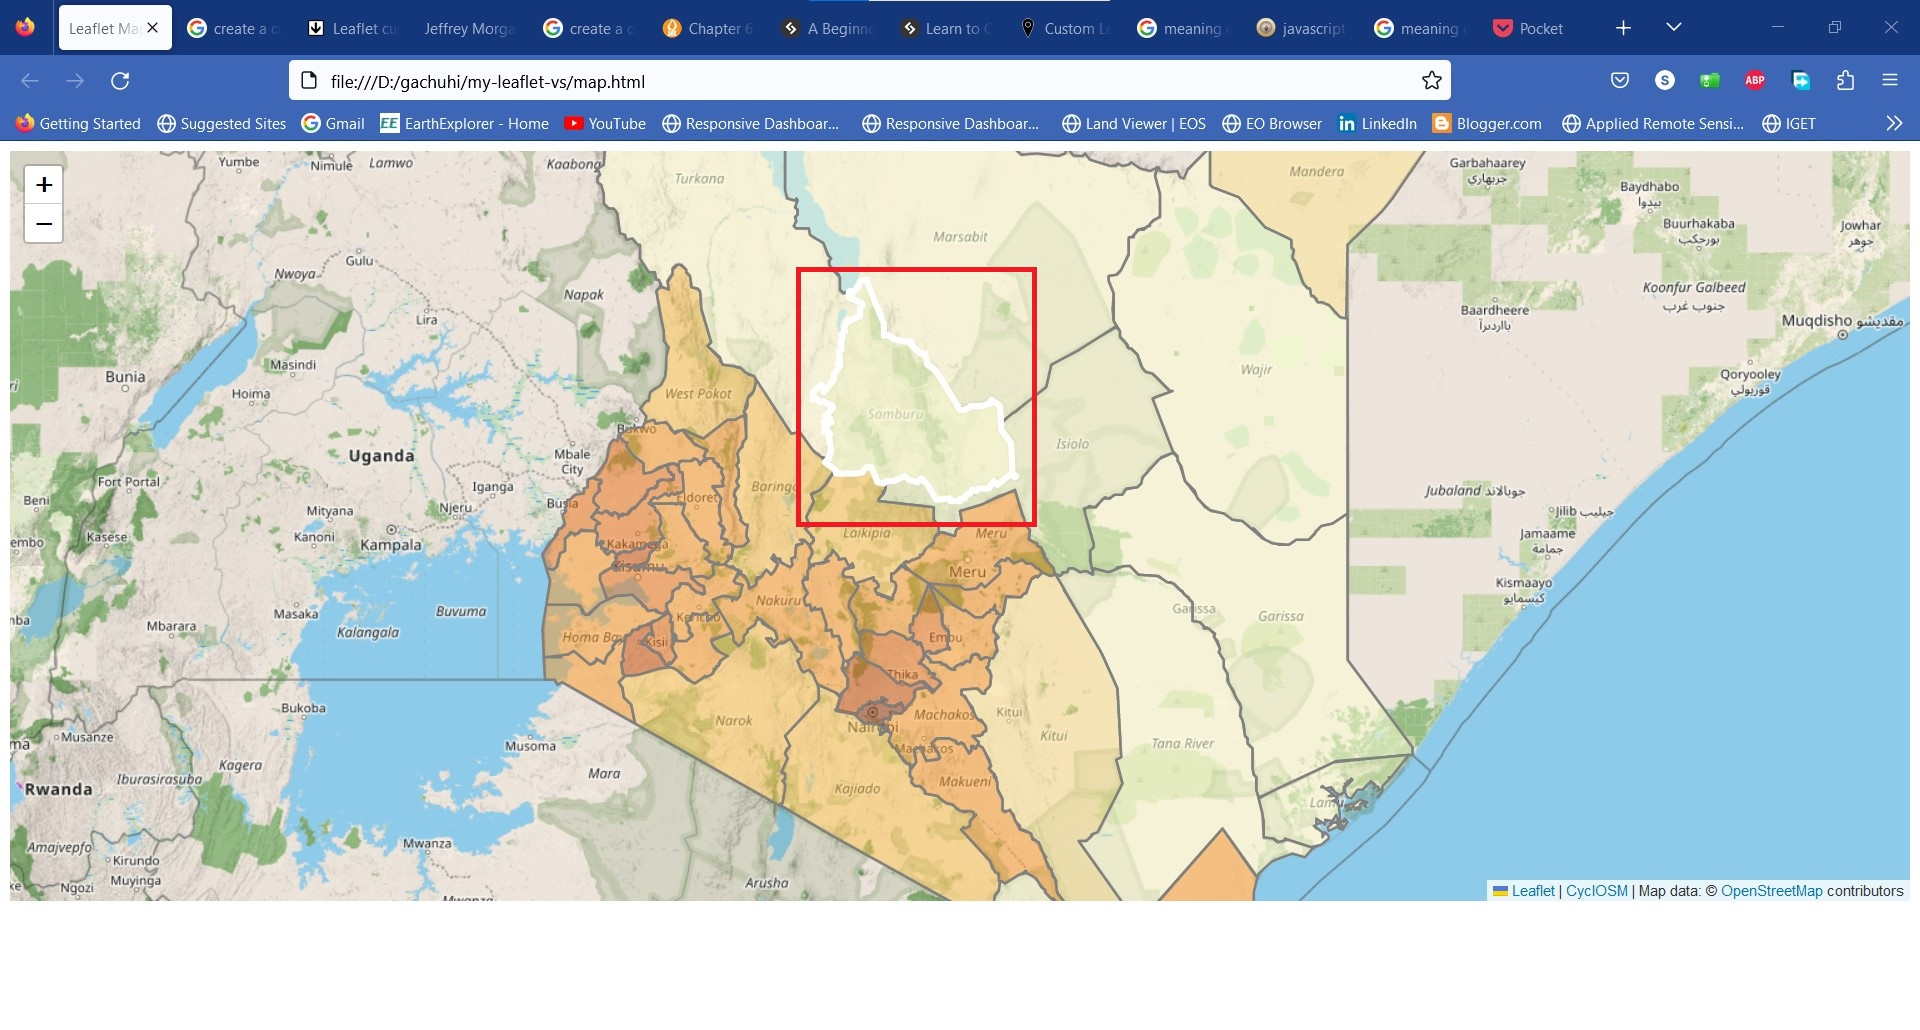
\includegraphics{../images/highlightable-map.jpg}

Your code within the \texttt{fetch} API should look like this.

\begin{verbatim}
fetch("https://raw.githubusercontent.com/sammigachuhi/geojson_files/main/counties_json.json")
    .then((response) =>{
        return response.json()
    })
    .then((data) => {
        var geojson;
        geojson = L.geoJson(data, {
            style: style,
            onEachFeature: ((feature, layer) => {
                layer.on('mouseover', ((e) => {  // highlight county on mouse hover
                    var layer = e.target;
                
                    layer.setStyle({
                        weight: 5,
                        color: '#FFFFFF',
                        dashArray: '',
                        fillOpacity: 0.7
                    });
                
                    layer.bringToFront();
                }))

                layer.on('mouseout', function () { // return to original symbology upon mouse hover out
                    geojson.resetStyle(this);
                })

                layer.on('click', ((e) => {  // Zoom to county upon clicking it
                    map.fitBounds(e.target.getBounds())
                }))

            })
        }).addTo(map);
    })
    .catch((error) => {
        console.log(`This is the error: ${error}`)
    })
\end{verbatim}

\hypertarget{creating-a-custom-info}{%
\section{Creating a custom info}\label{creating-a-custom-info}}

Our choropleth map works perfectly but lacks some interactivity. How about complementing it with an information interface next to it? Custom info controls are one way to do that. Think of a control as an UI element that allows interactivity. For our choropleth map, we want the custom control info to provide details of the name, total population and population density of each county hovered over.

\begin{verbatim}
// Add control
var info = L.control();

info.onAdd = function (map) {
    this.div = L.DomUtil.create('div', 'info');
    this.update();
    return this.div;
};

// Method that we will use to update the control based on feature properties passed
info.update = function (props) {
    this.div.innerHTML = '<h4>Kenya Population Density</h4>' + (props ? 
        '<b>' + props.ADM1_EN + '</br><br />' + 'Total Population' + '<br>' + props.County_pop + '<br> <br>' + 
        props.Pop_Density + ' people / km<sup>2</sup>': 'Hover over state')
};

info.addTo(map);
\end{verbatim}

Okay. Let's go through the above code bit by bit as best as we (hopefully!) can.

\begin{verbatim}
var info = L.control();
\end{verbatim}

The above creates a variable \texttt{info} that holds the base class \texttt{L.control()} for all map controls. For example, in \texttt{L.control.zoom}, the \texttt{L.control} class creates a zoom control in the map.

\begin{verbatim}
info.onAdd = function (map) {
    this.div = L.DomUtil.create('div', 'info');
    this.update();
    return this.div;
};
\end{verbatim}

The above code returns the DOM element for the control and creates a \texttt{\textless{}div\textgreater{}} of class \texttt{info}. This is done through the help of \texttt{L.DomUtil} which, according to the Leaflet website, provides utility functions to work with the Document Object Model (DOM)\footnote{The Document Object Model (DOM) is the data representation of the objects that comprise the structure and content of a document on the web.}. Actually, this new \texttt{\textless{}div\textgreater{}} of class \texttt{info} is created when you fire up your browser but will only exist in your browser. Don't expect it to magically appear in your static \texttt{map.html} file.

\begin{Shaded}
\begin{Highlighting}[]
\NormalTok{knitr}\SpecialCharTok{::}\FunctionTok{include\_graphics}\NormalTok{(}\FunctionTok{rep}\NormalTok{(}\StringTok{\textquotesingle{}D:/gachuhi/my{-}leaflet/images/div{-}info{-}element.jpg\textquotesingle{}}\NormalTok{))}
\end{Highlighting}
\end{Shaded}

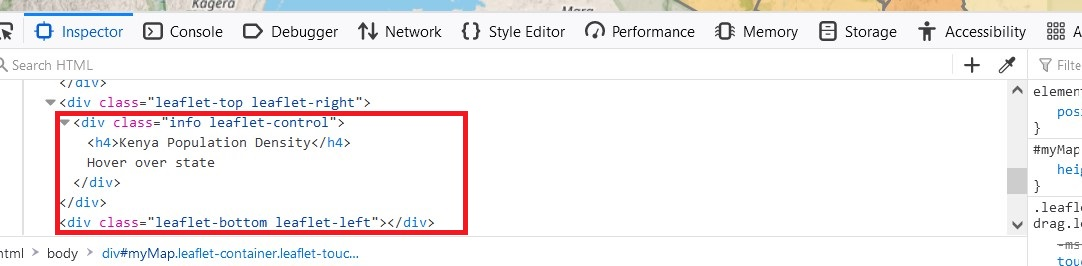
\includegraphics{../images/div-info-element.jpg}

In the aboe image, the \texttt{\textless{}div\textgreater{}} class bounded in red wasn't there before introducing the function containing \texttt{L.DomUtil}. Moving on forward, \texttt{this.update()} simply updates the content of the custom info control with the attributes of every newly clicked county.

\begin{verbatim}
// Method that we will use to update the control based on feature properties passed
info.update = function (props) {
    this.div.innerHTML = '<h4>Kenya Population Density</h4>' + (props ? 
        '<b>' + props.ADM1_EN + '</br><br />' + 'Total Population' + '<br>' + props.County_pop + '<br> <br>' + 
        props.Pop_Density + ' people / km<sup>2</sup>': 'Hover over state')
};

info.addTo(map);
\end{verbatim}

The above function updates the Leaflet map with the name, population and population density for each county. This function is passed to the variable \texttt{info.update} and thereafter added to the map using the method \texttt{addTo}. Inside this function exists the \texttt{this.div.innerHTML}. The purpose of \texttt{innerHtml} is to return the HTML content of an element. Since our map is rendered in a HTML page, the features will be returned as HTML.

Because the custom control info is a UI element, we need to set up its symbology in our CSS file. Paste the following to your \texttt{styles.css} file.

You may ask, ``I thought I don't have to put CSS styles to Leaflet because it seems to come with all batteries included, style 'n all''.

I get your point, but remember we created a new \texttt{\textless{}div\textgreater{}} called \texttt{info} that appears when our browser is powered up. And since this \texttt{\textless{}div\ class="info\ ..."\textgreater{}} must appear when the browser is powered up, CSS styles must be used to define its looks as well.

\begin{verbatim}
.info {
    padding: 6px 8px;
    font: 14px/16px Arial, Helvetica, sans-serif;
    background: white;
    background: rgba(255,255,255,0.8);
    box-shadow: 0 0 15px rgba(0,0,0,0.2);
    border-radius: 5px;
}

.info h4 {
    margin: 0 0 5px;
    color: #777;
}
\end{verbatim}

\hypertarget{create-a-legend}{%
\section{Create a legend}\label{create-a-legend}}

Having created a custom control info, the following code creates the legend.

\begin{verbatim}
var legend = L.control({position: 'bottomright'});

legend.onAdd = function (map) {
    var div = L.DomUtil.create('div', 'info legend'),
    grades = [0, 25, 50, 100, 400, 700, 1400],
    labels = [];

    // loop through our density intervals and generate a label with a colored square for each interval
    for (var i = 0; i < grades.length; i++) {
        div.innerHTML += 
            '<i style="background:' + getColor(grades[i] + 1) + '"></i> ' + 
            grades[i] + (grades[i + 1] ? '&ndash;' + grades[i + 1] + '<br>' : '+');
    }
    return div;
}

legend.addTo(map);
\end{verbatim}

Obviously the position of our legend is set using the \texttt{position} option in \texttt{L.control(\{position:\ \textquotesingle{}bottomright\textquotesingle{}\});}.

Apart from the other elements we discussed in our custom control info, we set the color interval of our legend through the \texttt{grades} array. The \texttt{for} loop that follows iterates through the grades array creating a color box for each interval.

Honestly, the code to create the legend color scheme is quite complicated. It has actually been copy pasted from the one in the Leaflet choropleth tutorial. The strangely looking \texttt{\&ndash} within the \texttt{for} loop of creating colors is simply how a hyphen (-) is written in HTML. But anyway, getting back to the \texttt{for} loop, it essentially creates a range within each interval, such as 0 - 25, 25 - 50 and so on. This takes place after the \texttt{?} ternary operator discussed earlier. Once it reaches the end of the loop, that is, it goes out of the range, the \texttt{+} is appended to the last value from our \texttt{grades} array. This last bit is made possible due to the \texttt{:} which returns values that are false in JavaScript.

The legend also needs its CSS properties or else it will not appear in the browser. The \texttt{\textless{}div\textgreater{}} class of \texttt{info\ legend} is also created when the browser fires up. You may be wondering why \texttt{info\ legend} and not just \texttt{legend}. Well, dear Golden Eye, the properties of \texttt{.info} class, such as background color and others are also inherited by the \texttt{legend} class by virtue of the browser, as in the case of HTML files, reading the CSS in a top-down format. The \texttt{legend} class will only override those properties that also appear in the \texttt{info\ legend} class. We also specify the CSS properties for the color intervals and text through the \texttt{.legend\ i} class.

Here's the CSS anyway.

\begin{verbatim}
.legend {
    line-height: 18px;
    color: #555;
}
.legend i {
    width: 18px;
    height: 18px;
    float: left;
    margin-right: 8px;
    opacity: 0.7;
}

\end{verbatim}

The legend is done and is finally added to the map.

\begin{Shaded}
\begin{Highlighting}[]
\NormalTok{knitr}\SpecialCharTok{::}\FunctionTok{include\_graphics}\NormalTok{(}\StringTok{\textquotesingle{}D:/gachuhi/my{-}leaflet/images/choropleth{-}legend.jpg\textquotesingle{}}\NormalTok{)}
\end{Highlighting}
\end{Shaded}

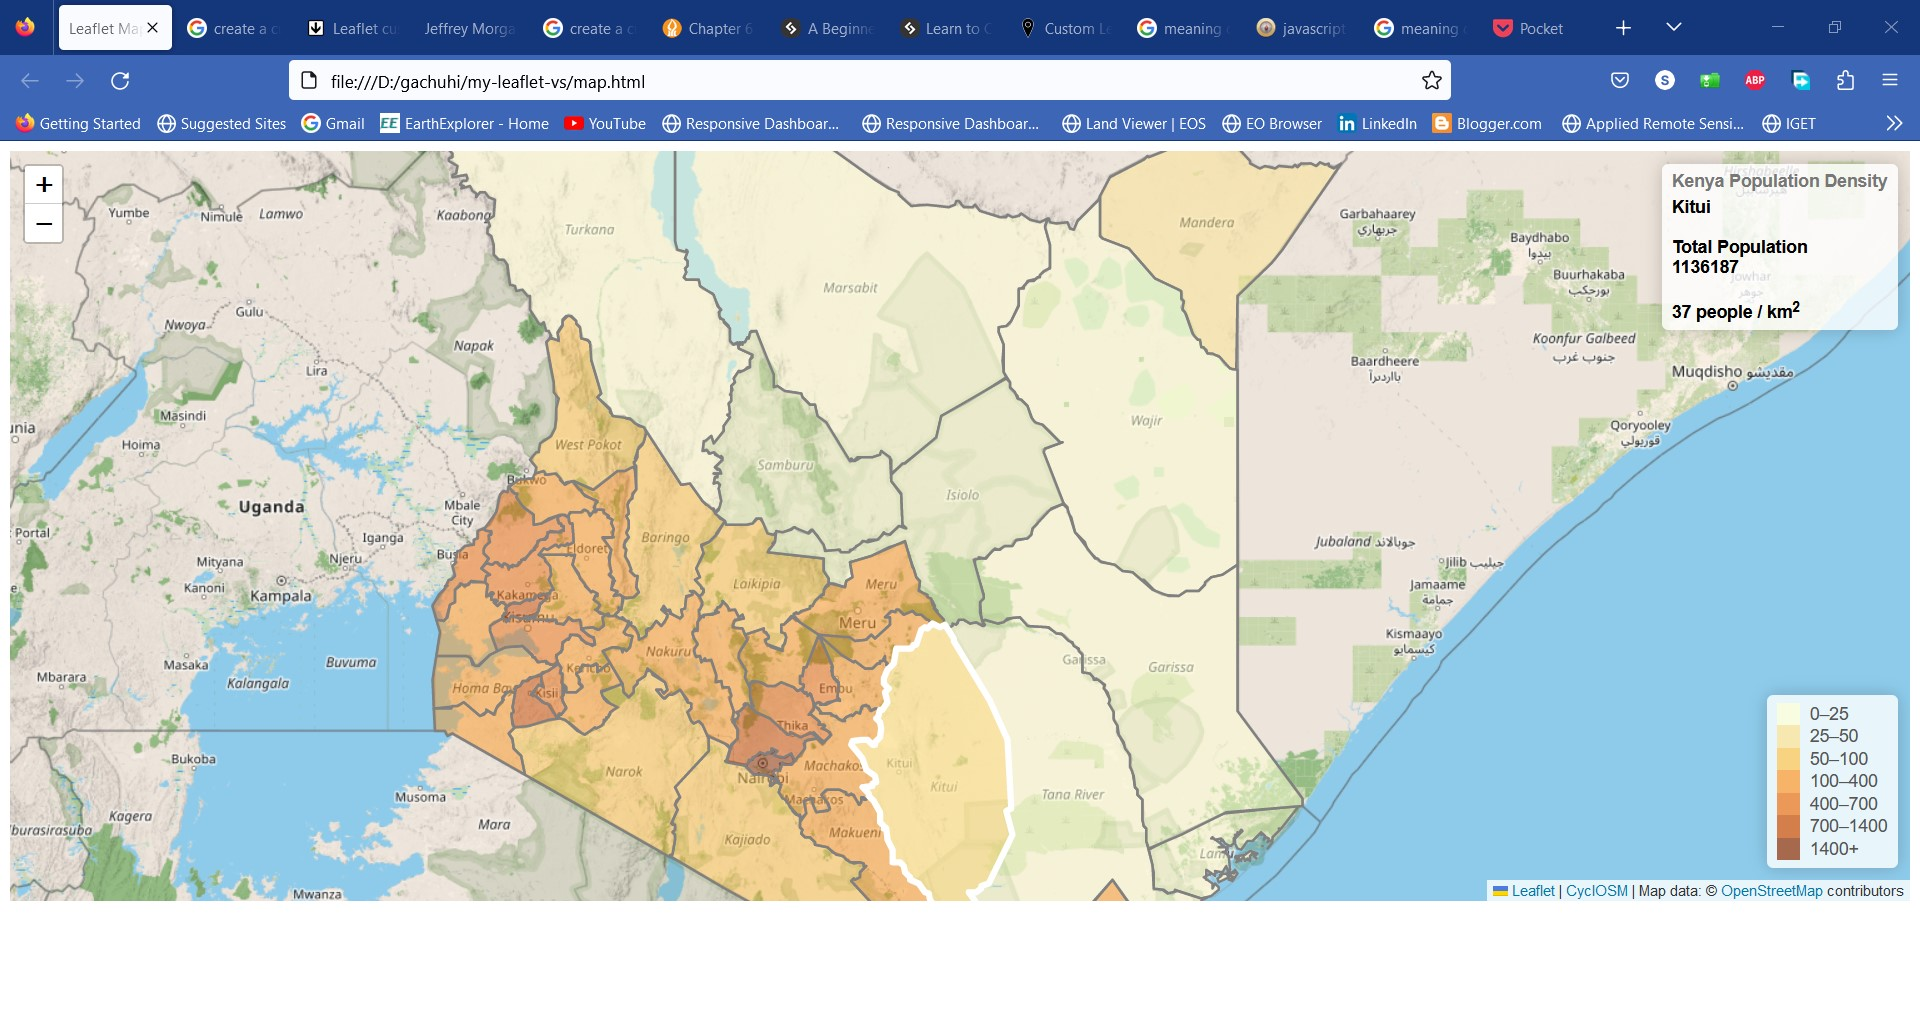
\includegraphics{../images/choropleth-legend.jpg}

The full code files are available from \href{https://github.com/sammigachuhi/my-leaflet-project/tree/main/my-leaflet-code/chapter-7-creating-interactive-choropleth-map}{here}.

When creating choropleth maps, aim for challenging and impacting the reader rather than merely informing.

\hypertarget{summary-6}{%
\section{Summary}\label{summary-6}}

This chapter was long and hard if not confusing. Nevertheless, here's our take home from this chapter:

\begin{itemize}
\item
  Choropleth maps are maps whose whose geographical areas or regions are colored, shaded or patterned in relation to a data variable. Good examples of choropleth maps are national population maps.
\item
  Ternary operators are short forms of the \texttt{if...else} statement. In a ternary operator, any statement to the right of the \texttt{?} is returned as true if it agrees with the value to the left of the \texttt{?}. Conversely,
  any value after the colon \texttt{:} is returned if the value to the right \texttt{?} is false.
\item
  \texttt{style} is a special key in the \texttt{L.geoJson} class that applies custom styles to each layer in the GeoJSON file.
\item
  \texttt{mouseover} is an event listener that triggers a certain action when
  a screen pointer is over a certain feature.
\item
  We can reset features back to their defaults using \texttt{resetStyle}.
\item
  The \texttt{L.control()} class is the base class for enabling most Leaflet controls. For example, the \texttt{L.control.zoom} creates the zoom controls.
\item
  \texttt{L.control()} can also be used to customize the appearance and information displayed by the legend.
\end{itemize}

\hypertarget{layer-groups-and-controls}{%
\chapter{Layer groups and controls}\label{layer-groups-and-controls}}

\hypertarget{purpose-of-layer-groups-and-controls}{%
\section{Purpose of layer groups and controls}\label{purpose-of-layer-groups-and-controls}}

Sometimes, one may wish for their webmap to consist of several baselayers or overlay maps. Suppose you want your Leaflet to have two basemap layers, and an additional overlay with the option of switching to any of them, how would you proceed?

\hypertarget{set-up-the-basemaps}{%
\section{Set up the basemaps}\label{set-up-the-basemaps}}

In order to create controls, we have to parse the objects holding our map variables into a \texttt{L.control.layers} class. Thereafter, the \texttt{L.controls.layers} class is used to parse the object values to the Leaflet map and create a UI control. To demonstrate this, open a new JavaScript file and name it \texttt{groups\_controls.js}. Insert the following code which will save our basemaps to the respective variables of \texttt{osm} and \texttt{cyclOSM}.

\begin{verbatim}
var osm = L.tileLayer('https://tile.openstreetmap.org/{z}/{x}/{y}.png', {
    maxZoom: 19,
    attribution: '&copy; <a href="http://www.openstreetmap.org/copyright">OpenStreetMap</a>'
});

var cyclOSM = L.tileLayer('https://{s}.tile-cyclosm.openstreetmap.fr/cyclosm/{z}/{x}/{y}.png', {
    maxZoom: 20,
    attribution: '<a href="https://github.com/cyclosm/cyclosm-cartocss-style/releases" title="CyclOSM - Open Bicycle render">CyclOSM</a> | Map data: &copy; <a href="https://www.openstreetmap.org/copyright">OpenStreetMap</a> contributors'
}); // the CyclOSM tile layer available from Leaflet servers
\end{verbatim}

We will pass the above two variables of \texttt{osm} and \texttt{cyclOSM} to the \texttt{L.map} class which has an option of \texttt{layers} in which one can parse the layers they wish to be displayed on the map.

\begin{verbatim}
var map = L.map('myMap', {
    layers: [osm, cyclOSM]
}).setView([-1.295287148, 36.81984753], 7);
\end{verbatim}

However, that will only add the first basemap variable --that for \texttt{osm} while blocking out that of \texttt{cylcOSM}. This is shown below.

\begin{Shaded}
\begin{Highlighting}[]
\NormalTok{knitr}\SpecialCharTok{::}\FunctionTok{include\_graphics}\NormalTok{(}\FunctionTok{rep}\NormalTok{(}\StringTok{\textquotesingle{}D:/gachuhi/my{-}leaflet/images/no{-}control.jpg\textquotesingle{}}\NormalTok{))}
\end{Highlighting}
\end{Shaded}

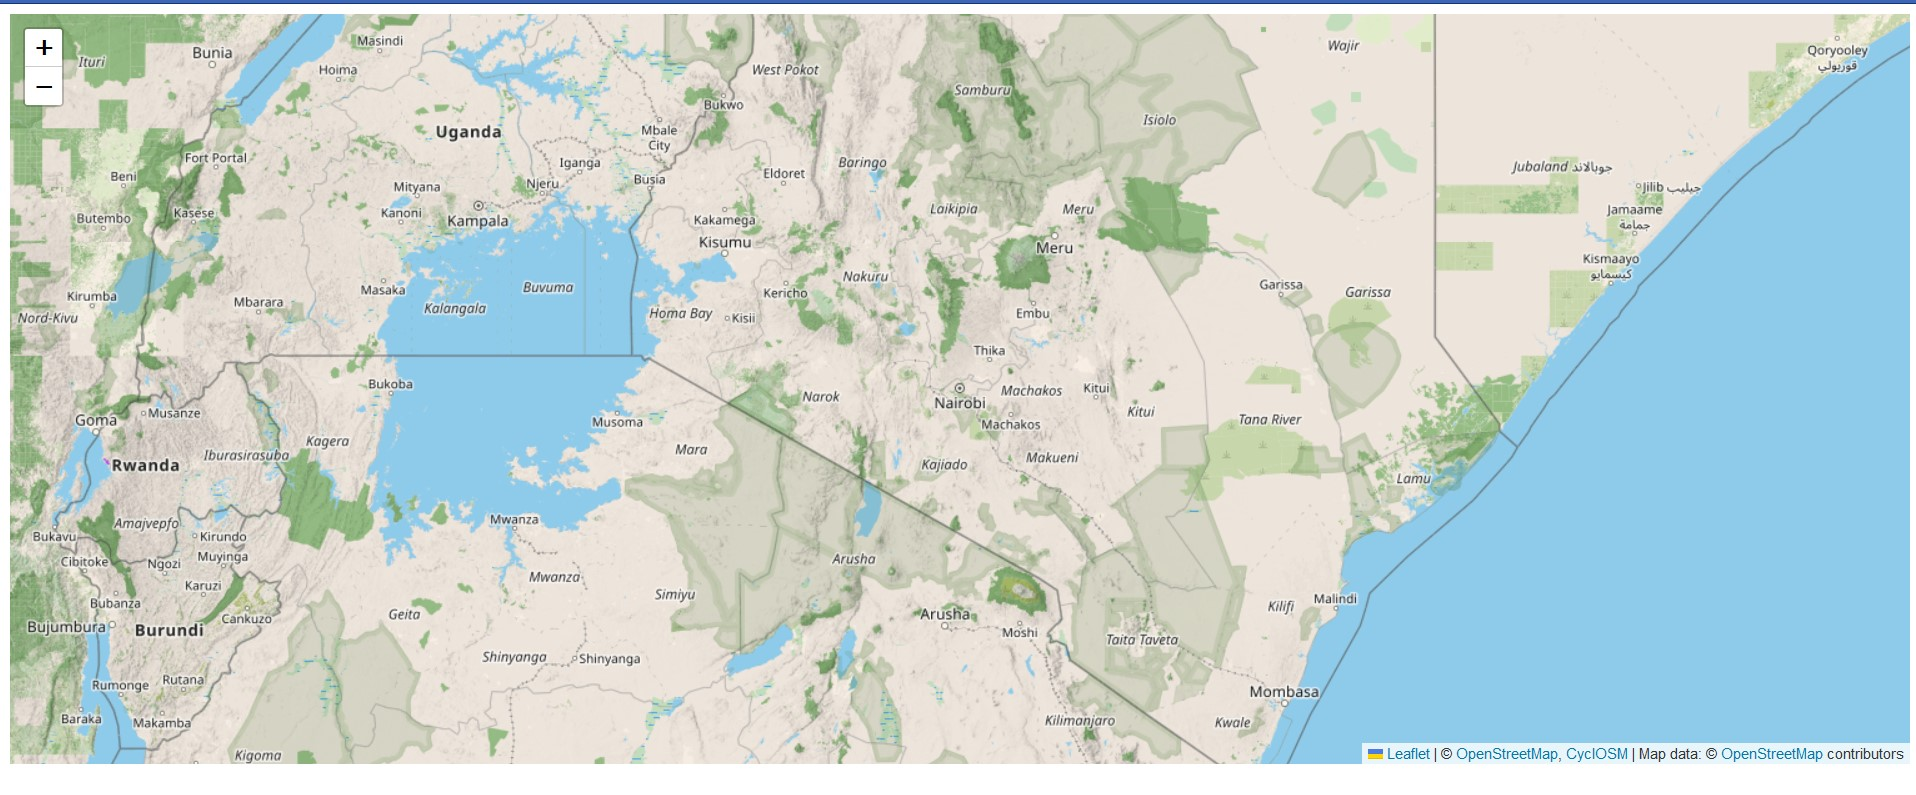
\includegraphics{../images/no-control.jpg}

\hypertarget{creating-the-controls}{%
\section{Creating the controls}\label{creating-the-controls}}

However, in order to give \texttt{cyclOSM} a fair chance, we need to store them in an object say \texttt{var\ basemaps} and parse it to \texttt{L.controls.layer} which shall create a checkbutton for each basemap. The below code does just that.

\begin{verbatim}
// Set object for the basemaps
var basemaps = {
    "OpenStreetMap": osm,
    'cycleOsm': cyclOSM,
}

L.control.layers(basemaps).addTo(map);

\end{verbatim}

This is the result you get.

\begin{Shaded}
\begin{Highlighting}[]
\NormalTok{knitr}\SpecialCharTok{::}\FunctionTok{include\_graphics}\NormalTok{(}\FunctionTok{rep}\NormalTok{(}\StringTok{\textquotesingle{}D:/gachuhi/my{-}leaflet/images/controls.jpg\textquotesingle{}}\NormalTok{))}
\end{Highlighting}
\end{Shaded}

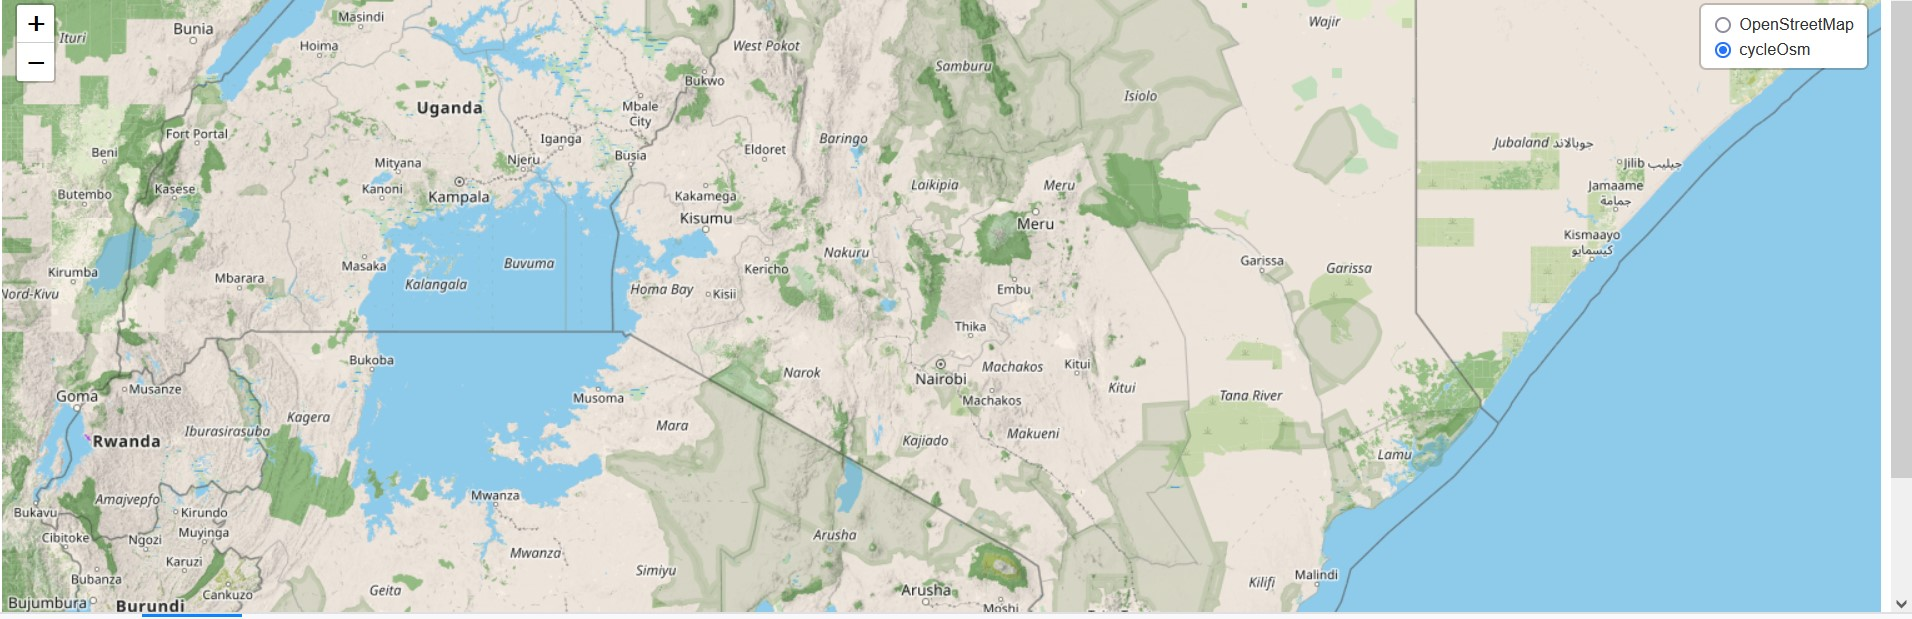
\includegraphics{../images/controls.jpg}

\hypertarget{adding-overlay-maps}{%
\section{Adding overlay maps}\label{adding-overlay-maps}}

Now we have seen how to add two or more basemaps to Leaflet and make all of them appear in the layer control. Adding an overlay map follows the same procedure as well.

The first overlay we would like to create is a choropleth map displaying the percentage of conventional households with access to main sewers as per the \href{https://housingfinanceafrica.org/app/uploads/VOLUME-IV-KPHC-2019.pdf}{2019 census}. For simplicity purposes and to bypass errors we faced, we shall reuse the Ajax plugin for fetching GeoJSON files from online servers. As a reminder, we load Ajax into Leaflet by inserting it to the following \texttt{\textless{}script\textgreater{}} tags of our \texttt{map.html}.

\begin{verbatim}
<script src="leaflet-ajax-gh-pages\dist\leaflet.ajax.js"></script>

<script src="leaflet-ajax-gh-pages\dist\leaflet.ajax.min.js"></script>
        <script src="leaflet-ajax-gh-pages\example\leaflet.spin.js"></script>
        <script src="leaflet-ajax-gh-pages\example\spin.js"></script> 
\end{verbatim}

Using \texttt{fetch} API to load the json file brought up several errors requiring out-of-the-box thinking to solve, but using the alternative Ajax plugin was a safe landing. The following chunks of code will add the color function and styling for our countrywide sanitation map. The resulting coloring function shall be parsed to the Ajax function.

\begin{verbatim}
//// Adding some color
function getColor(d) {
    return d > 20 ? '#3288bd' :
            d > 10 ? '#99d594' :
            d > 6 ? '#e6f598' :
            d > 4 ? '#fee08b' :
            d >  2 ? '#fc8d59':
                     '#d53e4f';
                       
}

// Function for setting color (using arrow function)
var style = ((feature)=> {
    return {
        fillColor: getColor(feature.properties.Human_waste_disposal),
        weight: 2,
        opacity: 1,
        color: 'gray',
        fillOpacity: 0.9
    }
})
\end{verbatim}

Now let's add the overlay map that will display the population's accessibility to main sewer sanitation services. Spoiler alert: the statistics are quite grim.

\begin{verbatim}
// Adding the first overlay - map of household access to main sewer
var countySanitation = new L.geoJson.ajax("https://raw.githubusercontent.com/sammigachuhi/geojson_files/main/counties_sanitation.json", {
    style: style
})
.bindPopup(function (layer) {
            return `<b>County Name: </b> ${layer.feature.properties.ADM1_EN} <br>
            <b>Total County Population: </b><br> 
            ${layer.feature.properties.County_pop.toString()} <br><br>
            <b>% of Conventional Households with access to main sewer: </b><br><br>
            ${layer.feature.properties.Human_waste_disposal.toString()}`
        }).addTo(map);
\end{verbatim}

Let's add an accompanying legend for the above map. If you worked through \protect\hyperlink{creating-an-interactive-choropleth-map}{Chapter 7} that dealt with interactive choropleths, some of the below code should look familiar.

\begin{verbatim}

// Create a legend
var legend = L.control({position: 'bottomright'});

legend.onAdd = function (map) {
    var div = L.DomUtil.create('div', 'info legend'),
    grades = [0, 2, 4, 6, 10, 20],
    labels = [];

    // loop through our density intervals and generate a label with a colored square for each interval
    for (var i = 0; i < grades.length; i++) {
        div.innerHTML += 
            '<i style="background:' + getColor(grades[i] + 1) + '"></i> ' + 
            grades[i] + (grades[i + 1] ? '&ndash;' + grades[i + 1] + '<br>' : '+');
    }
    return div;
}

legend.addTo(map);
\end{verbatim}

Now set an object to hold one of our two overlay maps.

\begin{verbatim}
var overlays = {
    'countySanitation': countySanitation,
}
\end{verbatim}

Finally parse the \texttt{overlays} object to the \texttt{L.controls.layer} class.

\begin{verbatim}
// Add layer controls
L.control.layers(basemaps, overlays).addTo(map);
\end{verbatim}

\begin{Shaded}
\begin{Highlighting}[]
\NormalTok{knitr}\SpecialCharTok{::}\FunctionTok{include\_graphics}\NormalTok{(}\FunctionTok{rep}\NormalTok{(}\StringTok{\textquotesingle{}D:/gachuhi/my{-}leaflet/images/controls{-}overlay.jpg\textquotesingle{}}\NormalTok{))}
\end{Highlighting}
\end{Shaded}

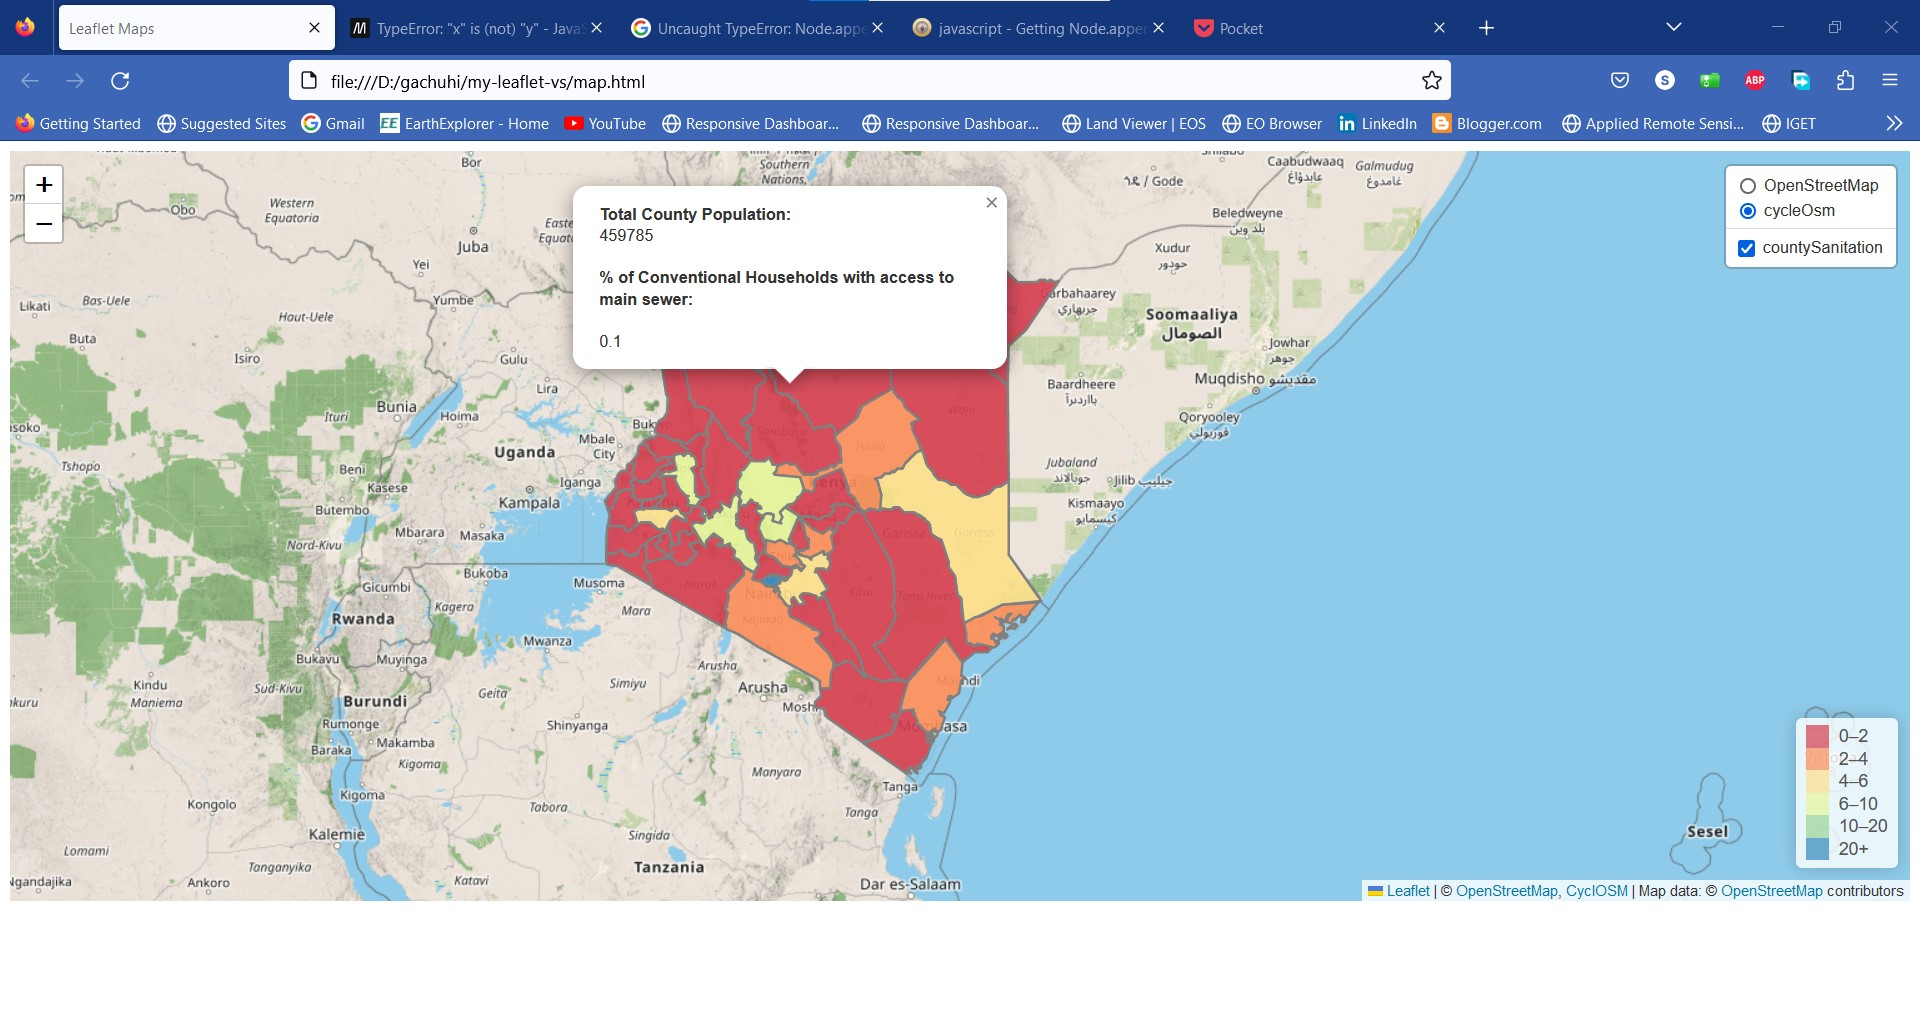
\includegraphics{../images/controls-overlay.jpg}

If you click in any one of the counties, you will see popups appear.

There is one more overlay we will add to our display to bring our experimentation with layer controls back full circle. Remember the GeoJSON of our \texttt{cities} variable? Let's call it back to action. But first let's load the custom icon markers that differentiate our cities based on population.

\begin{verbatim}
// Color icons
// Yellow Icon
var yellowIcon = new L.Icon({
    iconUrl: 'https://raw.githubusercontent.com/pointhi/leaflet-color-markers/master/img/marker-icon-2x-yellow.png',
    shadowUrl: 'https://cdnjs.cloudflare.com/ajax/libs/leaflet/0.7.7/images/marker-shadow.png',
    iconSize: [25, 41],
    iconAnchor: [12, 41],
    popupAnchor: [1, -34],
    shadowSize: [41, 41]
  });

// Orange Icon
var orangeIcon = new L.Icon({
    iconUrl: 'https://raw.githubusercontent.com/pointhi/leaflet-color-markers/master/img/marker-icon-2x-orange.png',
    shadowUrl: 'https://cdnjs.cloudflare.com/ajax/libs/leaflet/0.7.7/images/marker-shadow.png',
    iconSize: [25, 41],
    iconAnchor: [12, 41],
    popupAnchor: [1, -34],
    shadowSize: [41, 41]
  });

// Red Icon
var redIcon = new L.Icon({
    iconUrl: 'https://raw.githubusercontent.com/pointhi/leaflet-color-markers/master/img/marker-icon-2x-red.png',
    shadowUrl: 'https://cdnjs.cloudflare.com/ajax/libs/leaflet/0.7.7/images/marker-shadow.png',
    iconSize: [25, 41],
    iconAnchor: [12, 41],
    popupAnchor: [1, -34],
    shadowSize: [41, 41]
  });
\end{verbatim}

Let's load the \texttt{cities} GeoJSON with its icons.

\begin{verbatim}
var cities = L.geoJson.ajax("https://raw.githubusercontent.com/sammigachuhi/geojson_files/main/cities-geojson2.geojson.txt", {
    pointToLayer: function (feature, latlng) {
            if (feature.properties.Population <= 250000) {
              return L.marker(latlng, {
                icon: yellowIcon 
              });
            } else if (feature.properties.Population <= 800000) {
              return L.marker(latlng, {
                icon: orangeIcon 
              });
            } else {
              return L.marker(latlng, {
                icon: redIcon 
              });
            }
            
          }
}).bindPopup(function (layer) {
      return `City: ${layer.feature.properties.City},<br>
      Population: ${layer.feature.properties.Population}`;
    }).addTo(map);
    
\end{verbatim}

Add the \texttt{cities} variable as one of the keys to our \texttt{overlays} variable and finally parse the \texttt{overlays} object to \texttt{L.control.layers}.

\begin{verbatim}
// Set object for the overlay maps
var overlays = {
    'countySanitation': countySanitation,
    'cities': cities
}

// Add layer controls
L.control.layers(basemaps, overlays).addTo(map);
\end{verbatim}

In the \protect\hyperlink{creating-an-interactive-choropleth-map}{chapter 7}, we ended by saying that we strive to make our choropleths map challenge rather than merely inform. This looks like a sketchy map, but it clearly shows the discrepancy of access to basic sanitation services in a large portion of the population.

Finally, it seems changing the position of the \texttt{L.controls.layer} from its default top-right position is impossible. For example, setting the position to left, in the \texttt{L.controls.layer(basemap,\ overlaymap,\ \{position:\ \textquotesingle{}topleft\textquotesingle{}\})} results in the UI layers control disappearing completely off the map. This may likely be a yet to be reported bug.

\begin{Shaded}
\begin{Highlighting}[]
\NormalTok{knitr}\SpecialCharTok{::}\FunctionTok{include\_graphics}\NormalTok{(}\FunctionTok{rep}\NormalTok{(}\StringTok{\textquotesingle{}D:/gachuhi/my{-}leaflet/images/controls{-}all.jpg\textquotesingle{}}\NormalTok{))}
\end{Highlighting}
\end{Shaded}

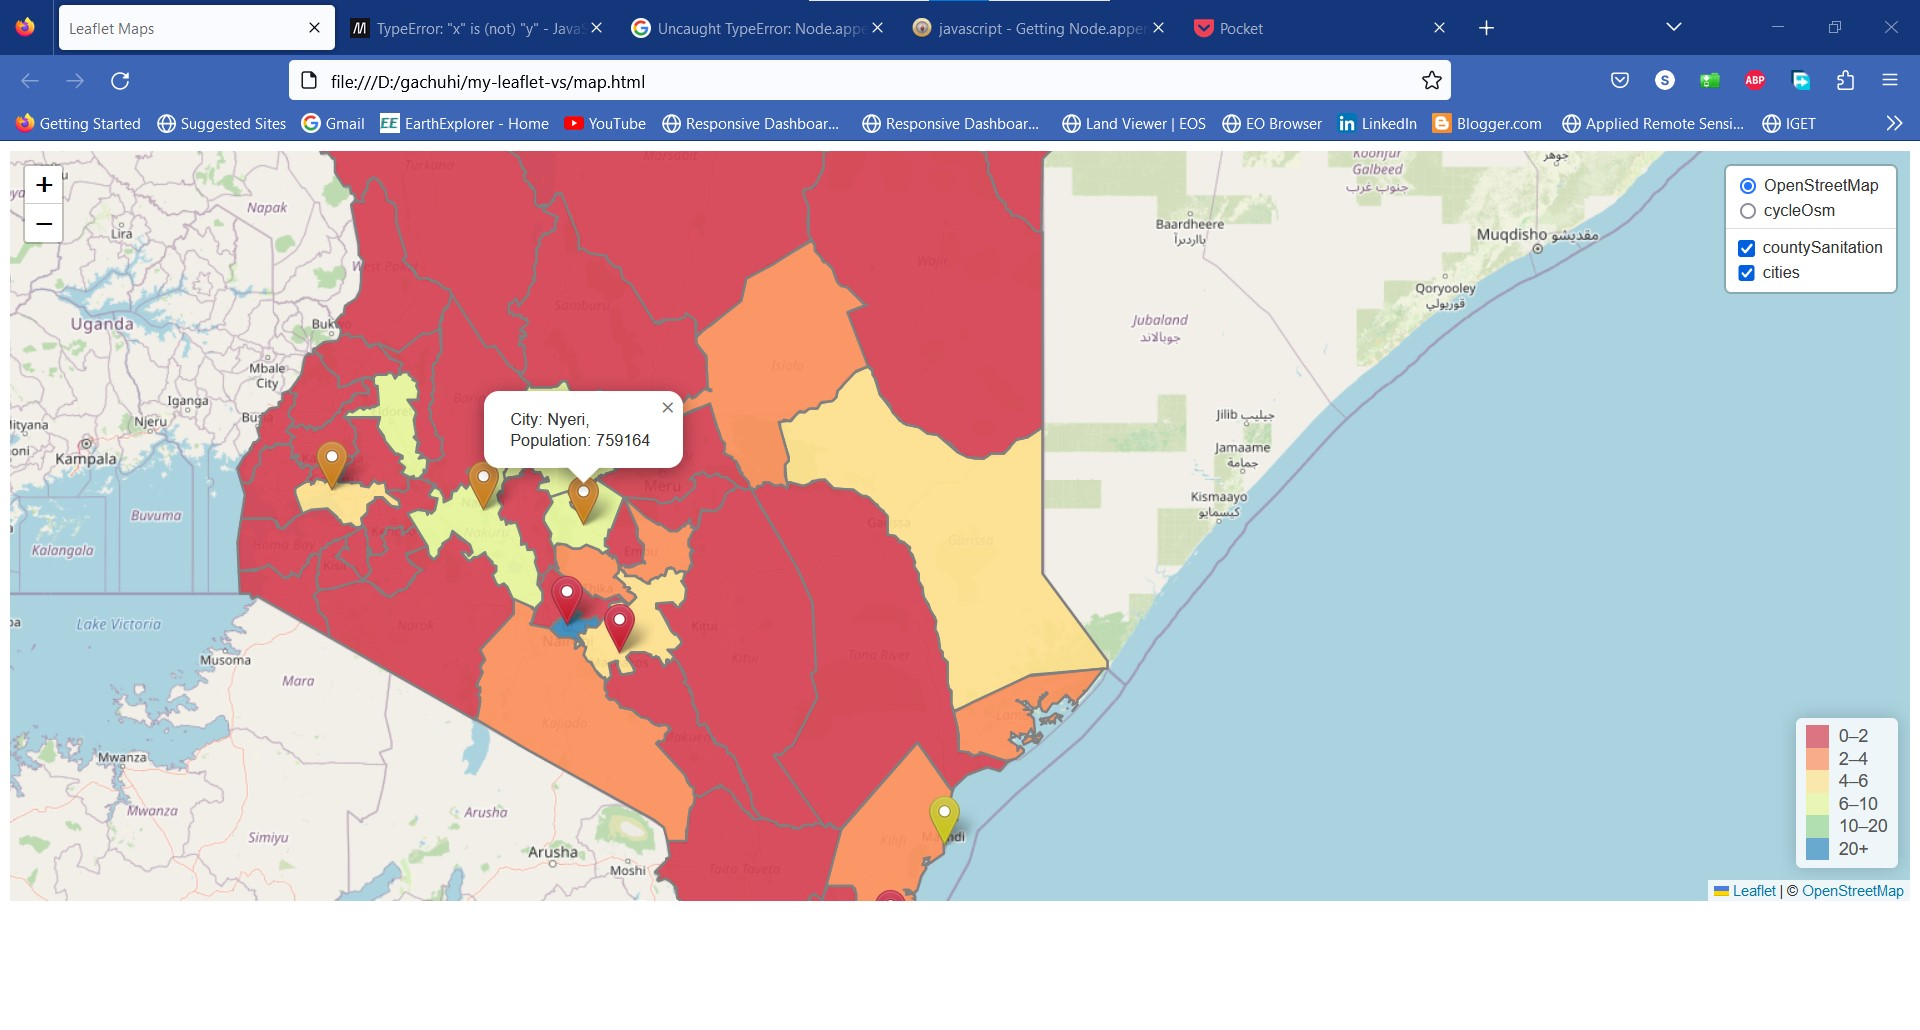
\includegraphics{../images/controls-all.jpg}

\hypertarget{add-a-scale-bar}{%
\section{Add a scale bar}\label{add-a-scale-bar}}

Scales are one of the key elements of any map. One may wonder what's their use in a webmap, but they are useful in estimating size and length of features. Adding a small reactive scale will not hurt!

\begin{verbatim}
// Add scale
L.control.scale({position:'bottomleft'}).addTo(map);
\end{verbatim}

\begin{Shaded}
\begin{Highlighting}[]
\NormalTok{knitr}\SpecialCharTok{::}\FunctionTok{include\_graphics}\NormalTok{(}\FunctionTok{rep}\NormalTok{(}\StringTok{\textquotesingle{}D:/gachuhi/my{-}leaflet/images/controls{-}scale.jpg\textquotesingle{}}\NormalTok{))}
\end{Highlighting}
\end{Shaded}

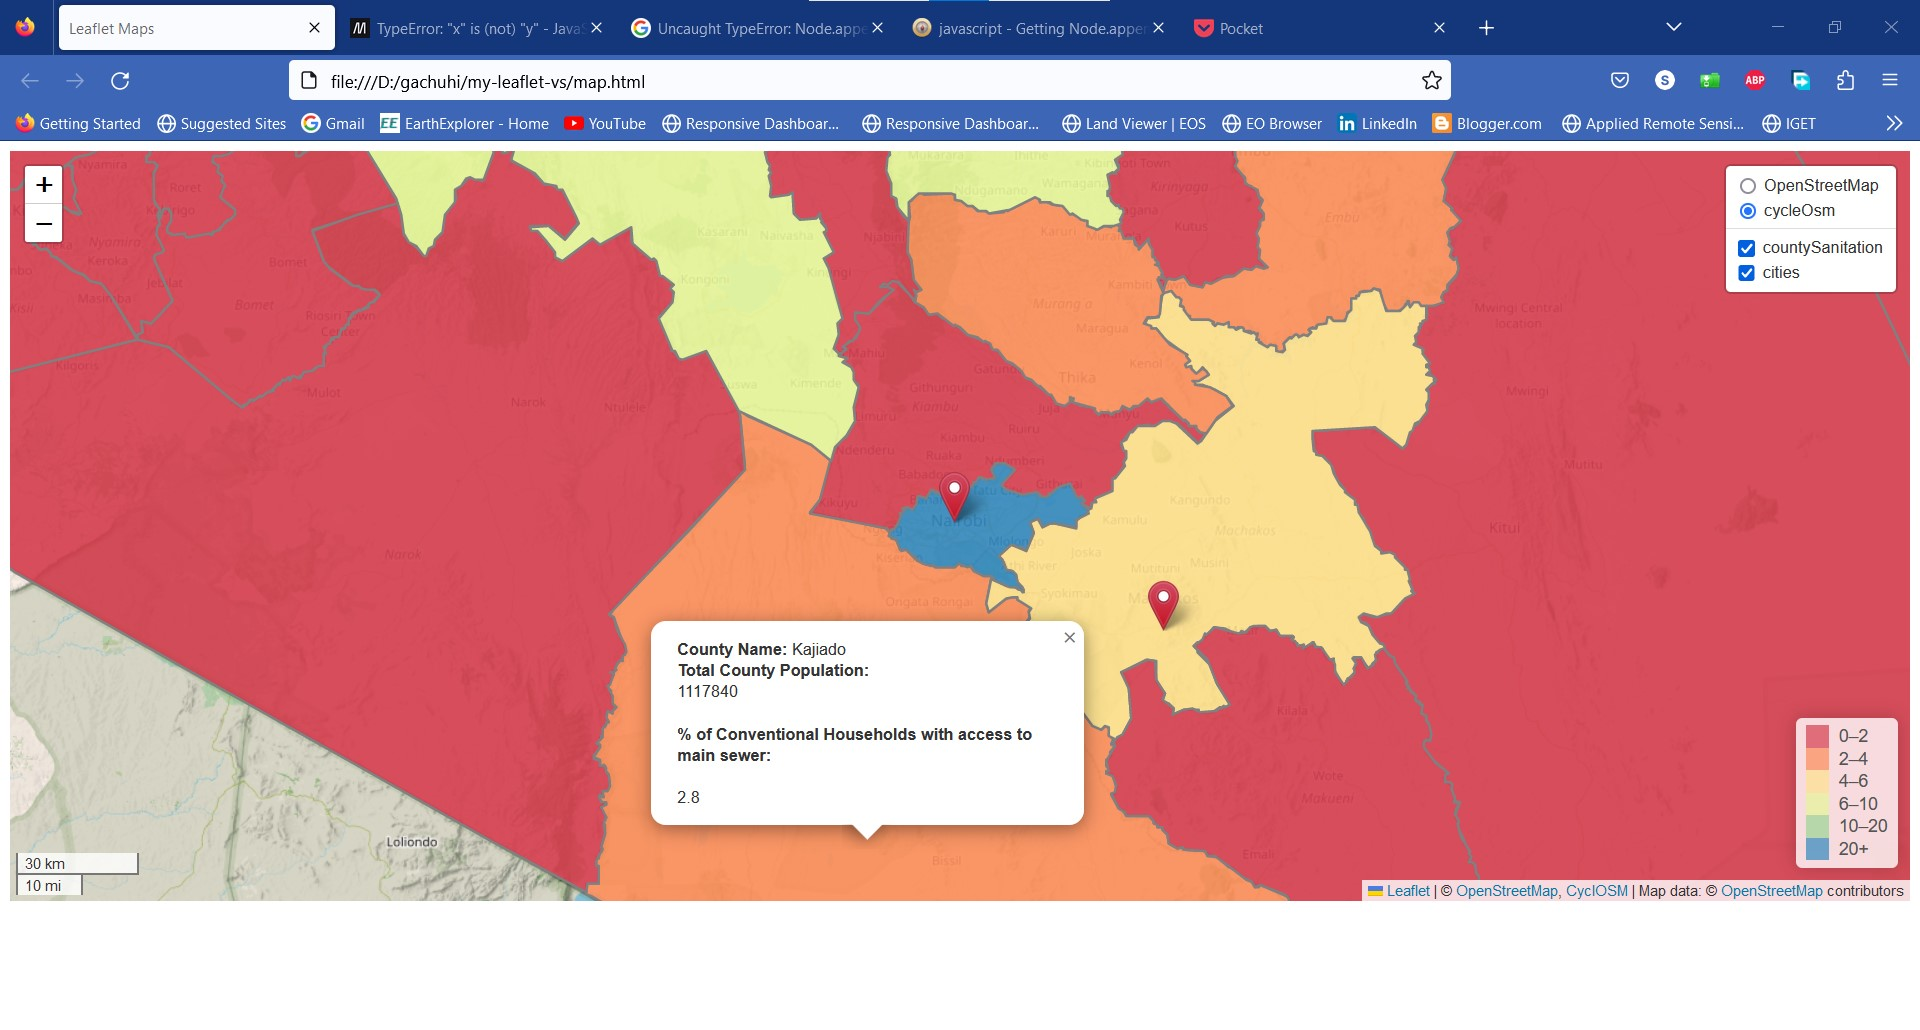
\includegraphics{../images/controls-scale.jpg}

All the files and scripts used in this chapter can be accessed \href{https://github.com/sammigachuhi/my-leaflet-project/tree/main/my-leaflet-code/chapter-8-layer_groups_and_controls}{here}.

\hypertarget{summary-7}{%
\section{Summary}\label{summary-7}}

Unlike paper maps, webmaps provide us the ability to include several basemaps and overlays all in one platform. Here's is what you have learnt from this chapter.

\begin{itemize}
\item
  Several basemaps and overlays can be parsed into Leaflet by holding the basemap and overlay variable names in a JavaScript dictionary object.
\item
  To create a layers control, parse the JavaScript object containing the basemap and overlay names to the \texttt{L.control.layers()} class.
\item
  GeoJSON features can also be parsed to the layer control. All that is needed is to save the function calling the GeoJSON file into a variable. For example, the Ajax function \texttt{var\ cities} was parsed to the \texttt{L.control.layers()} class.
\item
  Scales are useful for size and length estimation, even in webmaps. Leaflet provides the \texttt{L.control.scale} class to add custom scales to your webmap.
\end{itemize}

\hypertarget{heatmaps}{%
\chapter{Heatmaps}\label{heatmaps}}

\hypertarget{what-are-heatmaps}{%
\section{What are heatmaps?}\label{what-are-heatmaps}}

\href{https://www.gislounge.com/heat-maps-in-gis/}{Heatmaps} are a type of maps that geographically visualize locations with patterns of higher than average occurrence of particular variables say crime, disease, service centres and et cetera.

\hypertarget{loading-the-heatmap-plugin}{%
\section{Loading the heatmap plugin}\label{loading-the-heatmap-plugin}}

Leaflet does not have a prepackaged tool for drawing heatmaps. Instead, we have to use an external plugin by the name of \href{https://github.com/Leaflet/Leaflet.heat}{Leaflet.heat}. The link to the zipfile is available \href{https://codeload.github.com/Leaflet/Leaflet.heat/zip/refs/heads/gh-pages}{here}. Download and extract the folder to the same directory as your \texttt{map.html}.

Once you have extracted the zip file contents, open your \texttt{map.html} and add the following \texttt{\textless{}script\textgreater{}} tag within your \texttt{\textless{}head\textgreater{}} element.

\begin{verbatim}
<script src="Leaflet.heat-gh-pages\Leaflet.heat-gh-pages\dist\leaflet-heat.js"></script>
\end{verbatim}

Thereafter, we will have to think of a way of loading the GeoJson to a new JavaScript file called \texttt{heatmap.js}. This is where we shall write our heatmap code. You may think of using \texttt{fetch} or \texttt{L.geoJson.ajax} for this purpose but not so fast! The aforementioned methods failed in creating a heatmap. According to the documentation, heatmaps are created using \texttt{L.heatLayer}. Parsing \texttt{fetch} or \texttt{L.geoJson.ajax} into \texttt{L.heatLayer} to supposedly create a heatmap out of our GeoJSON points was not working. This is despite the two GeoJSON methods working well for various purposes in previous chapters. Thus, a new approach was needed.

After much internet searching, a code in Stack Overflow came to the rescue. However, it only works after inserting another Ajax plugin. Luckily no download is needed so insert this new \texttt{\textless{}script\textgreater{}} into your \texttt{map.html}.

\begin{verbatim}
<script src="https://ajax.googleapis.com/ajax/libs/jquery/2.1.4/jquery.min.js"></script>
\end{verbatim}

\hypertarget{creating-the-leaflet-heatmap}{%
\section{Creating the Leaflet heatmap}\label{creating-the-leaflet-heatmap}}

Let's call the usual suspects of adding a basemap.

\begin{verbatim}
var map = L.map('myMap').setView([0.3556, 37.5833], 6.5);

L.tileLayer('https://tile.openstreetmap.org/{z}/{x}/{y}.png', {
    attribution: '&copy; <a href="https://www.openstreetmap.org/copyright">OpenStreetMap</a> contributors'
}).addTo(map);
\end{verbatim}

Thereafter, we add the following large code chunks.

\begin{verbatim}
var geoJsonUrl = "https://raw.githubusercontent.com/sammigachuhi/geojson_files/main/selected_hospitals.json"

    var geojsonLayer = $.ajax({
    url : geoJsonUrl,
    dataType : 'json',
    jsonpCallback: 'getJson',
    success : console.log("Data successfully loaded!"),
    });

geoJson2heat = ((geojson) => {
        return geojson.features.map(function(feature) {
        return [parseFloat(feature.geometry.coordinates[1]), 
                parseFloat(feature.geometry.coordinates[0])];
        });
        });


$.when(geojsonLayer).done(function() {
        // var kill = L.geoJSON(geojsonLayer.responseJSON);
        var layer = geoJson2heat(geojsonLayer.responseJSON, 4);
        var heatMap = L.heatLayer(layer, { 
                radius: 40,
                blur: 10, 
                gradient: {
                        '0': 'Navy', '0.25': 'Navy',
                        '0.26': 'Green',
                        '0.5': 'Green',
                        '0.51': 'Yellow',
                        '0.75': 'Yellow',
                        '0.76': 'Red',
                        '1': 'Red'
                      },
                maxZoom: 13});
        map.addLayer(heatMap);
        });
\end{verbatim}

To give credit where it is due, the code chunks were taken from \href{https://gis.stackexchange.com/questions/337294/heatmap-with-geojson-leaflet-and-leaflet-heat-plugin?utm_source=pocket_reader}{this Stack Overflow question} and modified a bit. Let's do everyone some justice by going through the preceding code bit by bit.

\begin{verbatim}
var geoJsonUrl = "https://raw.githubusercontent.com/sammigachuhi/geojson_files/main/selected_hospitals.json"

    var geojsonLayer = $.ajax({
    url : geoJsonUrl,
    dataType : 'json',
    jsonpCallback: 'getJson',
    success : console.log("Data successfully loaded!"),
    });

\end{verbatim}

The \texttt{var\ geoJsonUrl} holds the link to our hospitals json file. The \texttt{var\ geojsonLayer} uses the Asynchronous Javascript And Xml (Ajax) method to load data from our Github server. If successful, we get the message ``Data successfully loaded!'' in our browser console.

\begin{verbatim}
geoJson2heat = ((geojson) => {
        return geojson.features.map(function(feature) {
        return [parseFloat(feature.geometry.coordinates[1]), 
                parseFloat(feature.geometry.coordinates[0])];
        });
        });
        
\end{verbatim}

The above code chunk is fairly easy to understand. The function passed to \texttt{geoJson2heat} uses the \texttt{map} method to iterate over every element, such as cities in the json file and retrieve the longitude and latitude coordinates. Notice the format has been inverted. Rather than {[}0{]}\ldots{} {[}1{]} for Lat-Lon, we use {[}1{]}\ldots{[}0{]}.

The final is a jQuery function that will return the desired heatmap layer.

\begin{verbatim}
$.when(geojsonLayer).done(function() {
        // var kill = L.geoJSON(geojsonLayer.responseJSON);
        var layer = geoJson2heat(geojsonLayer.responseJSON, 4);
        var heatMap = L.heatLayer(layer, { 
                radius: 40,
                blur: 10, 
                gradient: {
                        '0': 'Navy', '0.25': 'Navy',
                        '0.26': 'Green',
                        '0.5': 'Green',
                        '0.51': 'Yellow',
                        '0.75': 'Yellow',
                        '0.76': 'Red',
                        '1': 'Red'
                      },
                maxZoom: 13});
        map.addLayer(heatMap);
        });
\end{verbatim}

Honestly the last was a bit of a stretch since jQuery is hardly used in Leaflet or in normal JavaScript programming nowadays.

\begin{Shaded}
\begin{Highlighting}[]
\NormalTok{knitr}\SpecialCharTok{::}\FunctionTok{include\_graphics}\NormalTok{(}\FunctionTok{rep}\NormalTok{(}\StringTok{\textquotesingle{}D:/gachuhi/my{-}leaflet/images/heatmap.jpg\textquotesingle{}}\NormalTok{))}
\end{Highlighting}
\end{Shaded}

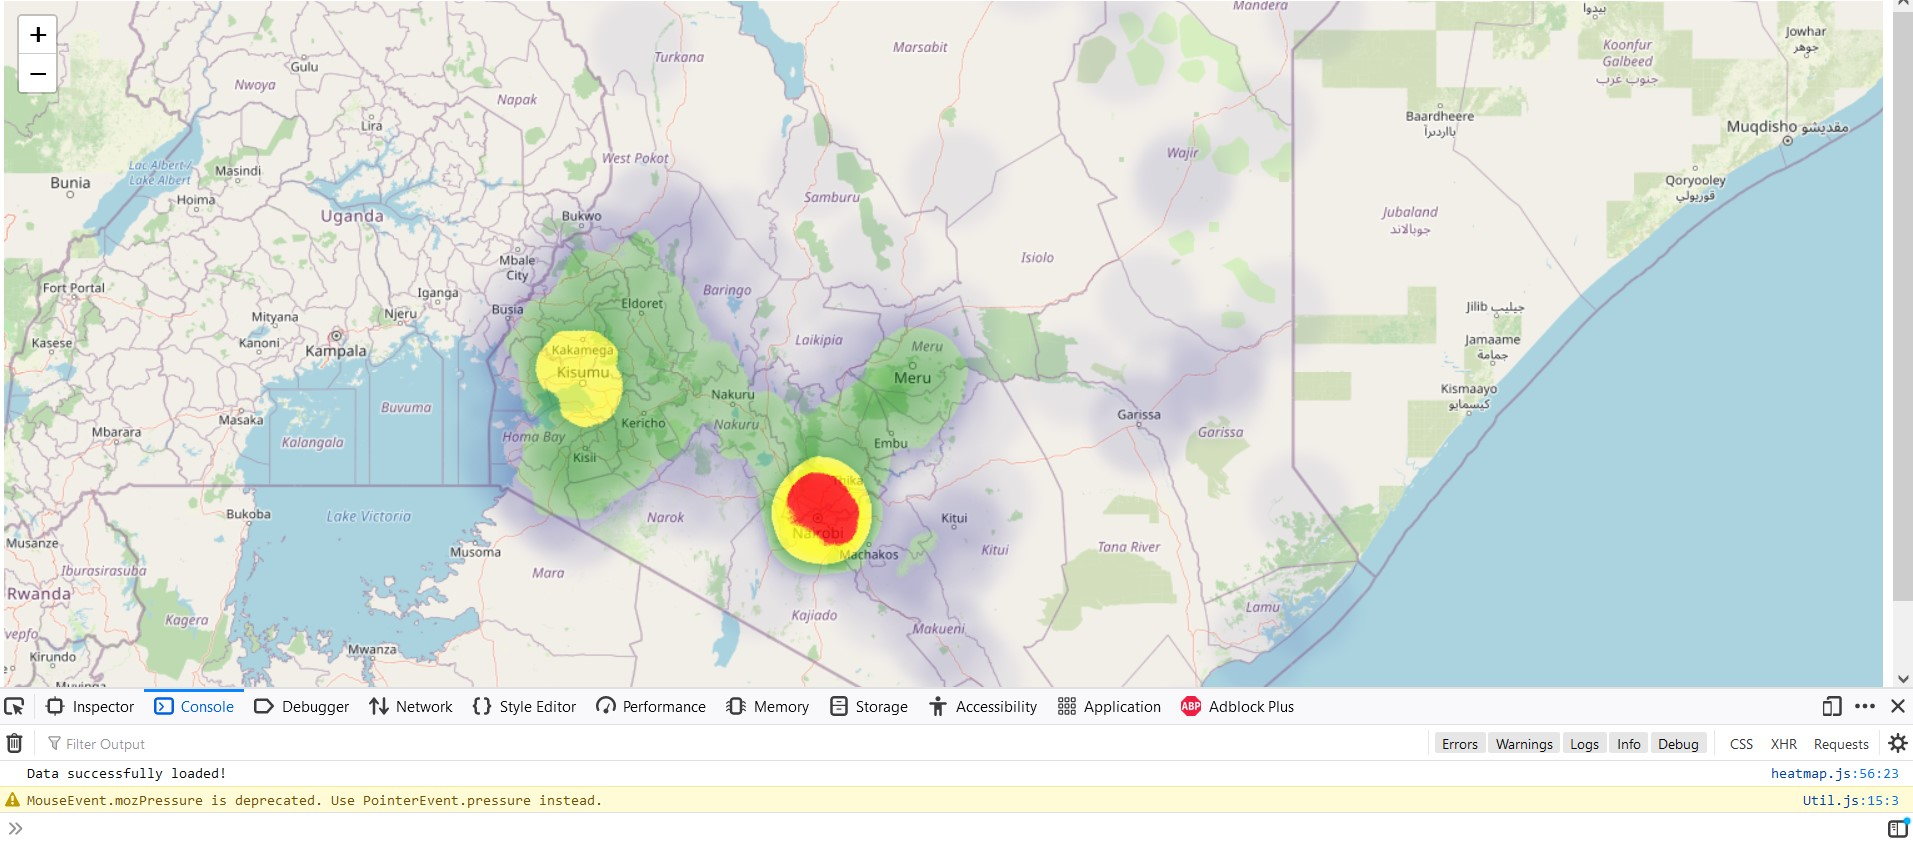
\includegraphics{../images/heatmap.jpg}

The full code files are available from \href{https://github.com/sammigachuhi/my-leaflet-project/tree/main/my-leaflet-code/chapter-9-Heatmaps}{here}.

\textbf{NB:} It should be noted that all manner of efforts were employed to \href{https://chat.openai.com/share/b76f0402-b1df-4585-997e-d2421cd68b6b}{create a heatmap} using \texttt{L.heatLayer}. The most promising seemed nesting the \texttt{L.heatLayer} within the simple \texttt{L.geoJson.ajax} class encountered numerous times so far. All attempts, including \href{https://chat.openai.com/share/7230d651-2959-407e-8e92-5500d470c8af}{asking ChatGPT} for a plausible solution, were unsuccessful.
\#\# Summary

Heatmaps are one of the simplest forms of maps in geography. They use color and hue to visualize the concentration of phenomena across space. Here are the take home notes from this chapter.

\begin{itemize}
\item
  Heatmaps are a type of maps that geographically visualize locations with patterns of higher than average occurrence of particular variables.
\item
  In order to draw heatmaps using Leaflet, we have to download the \texttt{Leaflet.heat} plugin. Thereafter, the path to the plugin is parsed to the \texttt{script} tag of your HTML file.
\item
  Apart from using L.heatLayer, the other alternative of creating heatmaps from GeoJSON data is through a combination of Ajax and jQuery.
\end{itemize}

\hypertarget{cluster-to-reduce-the-clutter}{%
\chapter{Cluster to reduce the clutter}\label{cluster-to-reduce-the-clutter}}

\hypertarget{a-map-full-of-clutter}{%
\section{A map full of clutter}\label{a-map-full-of-clutter}}

There comes a time when it is convenient to coalesce several points into a single multi-cluster point. Consider the following example: you have a GeoJSON file with over 10000 points of houses within a densely populated island of 5km by 5km, if by any chance such a scenario exists. Will you want to display such a gigantic number of points within such a small area? That would be an overkill! Moreover, the map would be incomprehensible to the viewer. Consider the following example we set up in a new JavaScript file which we fondly called \texttt{cluster-markers.js}.

\begin{verbatim}
var map = L.map('myMap').setView([-1.295287148, 36.81984753], 7);

L.tileLayer('https://tile.openstreetmap.org/{z}/{x}/{y}.png', {
    maxZoom: 19,
    attribution: '&copy; <a href="http://www.openstreetmap.org/copyright">OpenStreetMap</a>'
}).addTo(map);


url = 'https://raw.githubusercontent.com/sammigachuhi/geojson_files/main/selected_hospitals.json'

L.geoJson.ajax(url).addTo(map);

var markers = L.markerClusterGroup();
\end{verbatim}

The following is the result.

\begin{Shaded}
\begin{Highlighting}[]
\NormalTok{knitr}\SpecialCharTok{::}\FunctionTok{include\_graphics}\NormalTok{(}\FunctionTok{rep}\NormalTok{(}\StringTok{\textquotesingle{}D:/gachuhi/my{-}leaflet/images/clutter{-}points.jpg\textquotesingle{}}\NormalTok{))}
\end{Highlighting}
\end{Shaded}

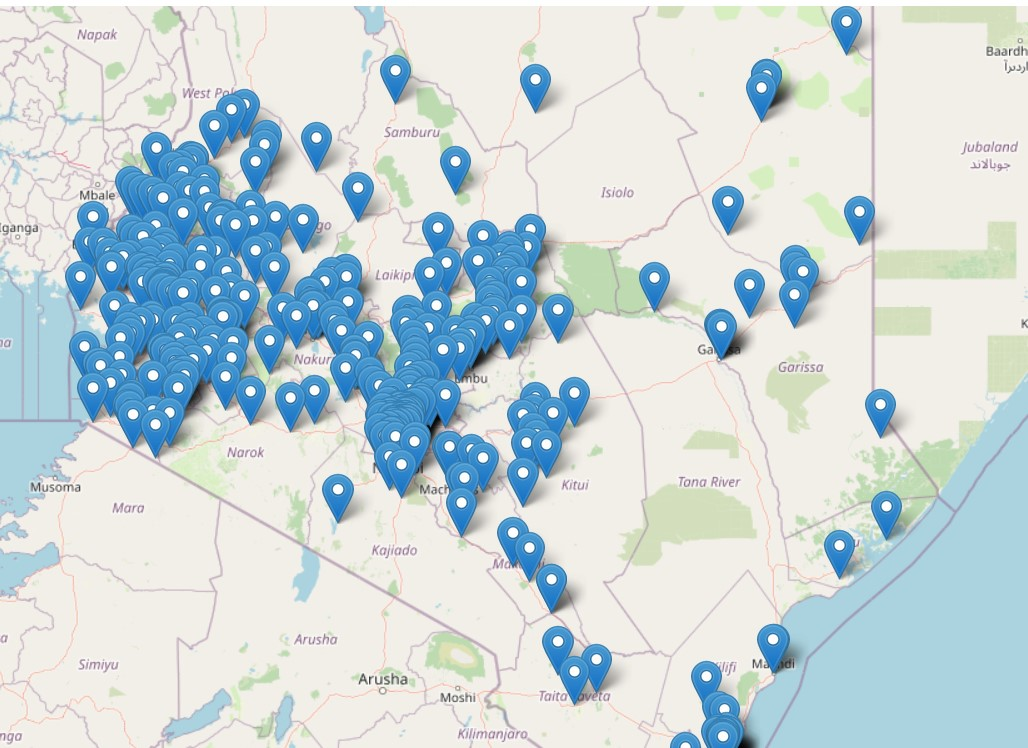
\includegraphics{../images/clutter-points.jpg}

Not good at all. The \texttt{Leaflet.markercluster} plugin is what transforms a clutter map into one of neatly arranged clustered marker points.

\hypertarget{preparations}{%
\section{Preparations}\label{preparations}}

Creating a cluster marker map is fairly easy. You will first have to insert the \texttt{Leaflet.markerCluster} plugin into \texttt{map.html}. The plugin is available from \href{https://github.com/Leaflet/Leaflet.markercluster/archive/refs/heads/master.zip}{here}. Insert the following \texttt{\textless{}script\textgreater{}} tag into the \texttt{\textless{}head\textgreater{}} element of your \texttt{map.html}.

\begin{verbatim}
<script src="Leaflet.markercluster-1.4.1\Leaflet.markercluster-1.4.1\dist\leaflet.markercluster.js"></script>
\end{verbatim}

You will also have to insert the \texttt{Leaflet.markercluster} CSS properties via the \texttt{\textless{}link\textgreater{}} tag too. Add the following \texttt{\textless{}link\textgreater{}} tag for \texttt{Leaflet.markercluster}. For legibility and clean code, place below the other \texttt{\textless{}link\textgreater{}} properties.

\begin{verbatim}
<link rel="stylesheet" href="Leaflet.markercluster-master\Leaflet.markercluster-master\dist\MarkerCluster.Default.css"> 
\end{verbatim}

Don't underestimate them. These CSS properties are necessary to style your cluster points in a nice way that's easy on the eye. It is also assumed you have already inserted the name of your JavaScript file, the \texttt{cluster-marker.js} within the \texttt{script} tag enclosed by the \texttt{\textless{}body\textgreater{}} element of your \texttt{map.html} file.

If you had done the small exercise at the beginning of the chapter, the following code should be present.

\begin{verbatim}
var map = L.map('myMap').setView([-1.295287148, 36.81984753], 7);

L.tileLayer('https://tile.openstreetmap.org/{z}/{x}/{y}.png', {
    maxZoom: 19,
    attribution: '&copy; <a href="http://www.openstreetmap.org/copyright">OpenStreetMap</a>'
}).addTo(map);


url = 'https://raw.githubusercontent.com/sammigachuhi/geojson_files/main/selected_hospitals.json'
\end{verbatim}

\hypertarget{behold-a-cluster-marker-map}{%
\section{Behold, a cluster marker map!}\label{behold-a-cluster-marker-map}}

Delete the \texttt{L.geoJson.ajax(url).addTo(map);}, we won't need it now. Our real work of creating a cluster marker map begins with the \texttt{markerClusterGroup} class. Let's proceed!

\begin{verbatim}
var markers = L.markerClusterGroup();
\end{verbatim}

We shall use Ajax again but this time round we shall parse in some functions to customize the appearance and functionalities of our GeoJson markers.

\begin{verbatim}

L.geoJson.ajax(url, {
    pointToLayer: ((feature, latLng) => {
        return markers.addLayer(L.circleMarker(latLng));
    }),

    onEachFeature: ((feature, layer) => {
        layer.bindPopup(`<b>Facility Name:</b> ${feature.properties.Facility_N} <br>
        <b>Type:</b> ${feature.properties.Type}`)
    })
}).addTo(map);
\end{verbatim}

Remember \texttt{pointToLayer} of Leaflet GeoJSON files? It defines how the GeoJson file will appear. The \texttt{pointToLayer} retrieves the Latitude-Longitude coordinates before finally creating circle markers out of them as enabled by \texttt{...return\ markers.addLayer(L.circleMarker(latLng))},

How about for \texttt{onEachFeature}? You can guess. It simply means-- \emph{O}n \emph{E}ach \emph{F}eature, \emph{do this and that}. In our case we bind a popup of facility name and type which will appear when a circle marker is clicked upon.

Actually, the above code sort of finished the work for us.

\begin{Shaded}
\begin{Highlighting}[]
\NormalTok{knitr}\SpecialCharTok{::}\FunctionTok{include\_graphics}\NormalTok{(}\FunctionTok{rep}\NormalTok{(}\StringTok{\textquotesingle{}D:/gachuhi/my{-}leaflet/images/cluster{-}marker{-}map.jpg\textquotesingle{}}\NormalTok{))}
\end{Highlighting}
\end{Shaded}

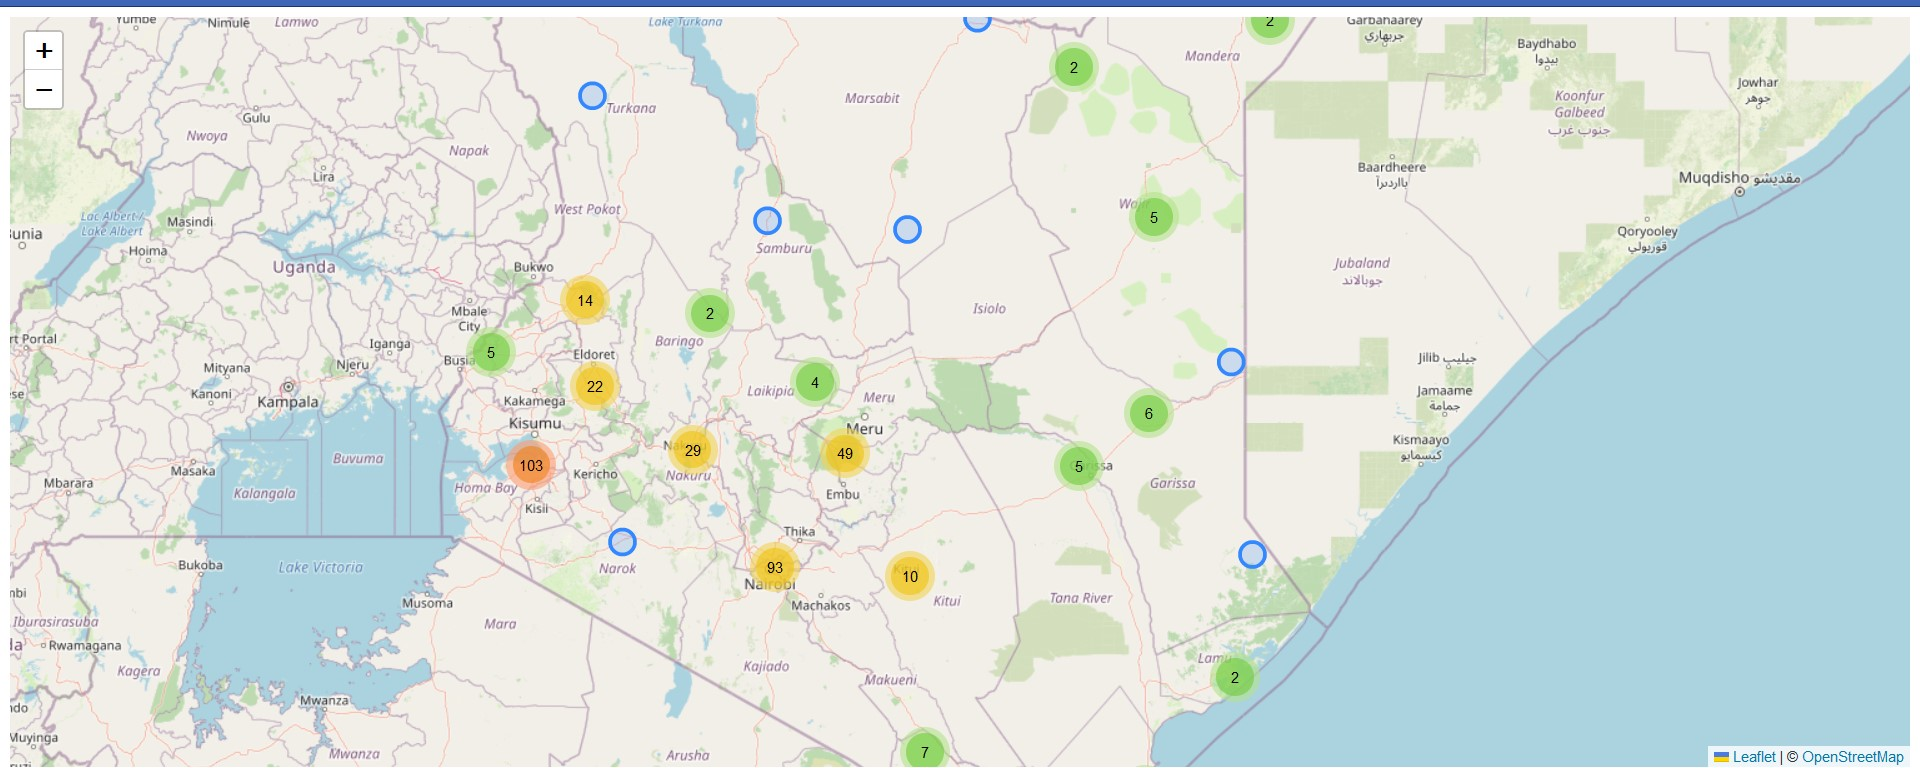
\includegraphics{../images/cluster-marker-map.jpg}

Zoom in and out and watch the circle markers \emph{spidefy} the individual points with a popup. I have restrained from tweaking the markers because the defaults are already good enough. See them from this \href{https://github.com/Leaflet/Leaflet.markercluster}{Github Page}.

However, as good practice, we need to add the \texttt{markers} global variable to the map. We do so by using the following code.

\begin{verbatim}
map.addLayer(markers)
\end{verbatim}

\texttt{addLayers}, just like the name suggests, adds the given layer to the map.

The \texttt{L.circleMarker} in the \texttt{pointToLayer} key of the Ajax function can be replaced with \texttt{L.marker()}. Below is how some spiderfied hospital markers look like, but they are less aesthetically pleasing than the circle markers.

\begin{Shaded}
\begin{Highlighting}[]
\NormalTok{knitr}\SpecialCharTok{::}\FunctionTok{include\_graphics}\NormalTok{(}\FunctionTok{rep}\NormalTok{(}\StringTok{\textquotesingle{}D:/gachuhi/my{-}leaflet/images/cluster{-}marker{-}plain.jpg\textquotesingle{}}\NormalTok{))}
\end{Highlighting}
\end{Shaded}

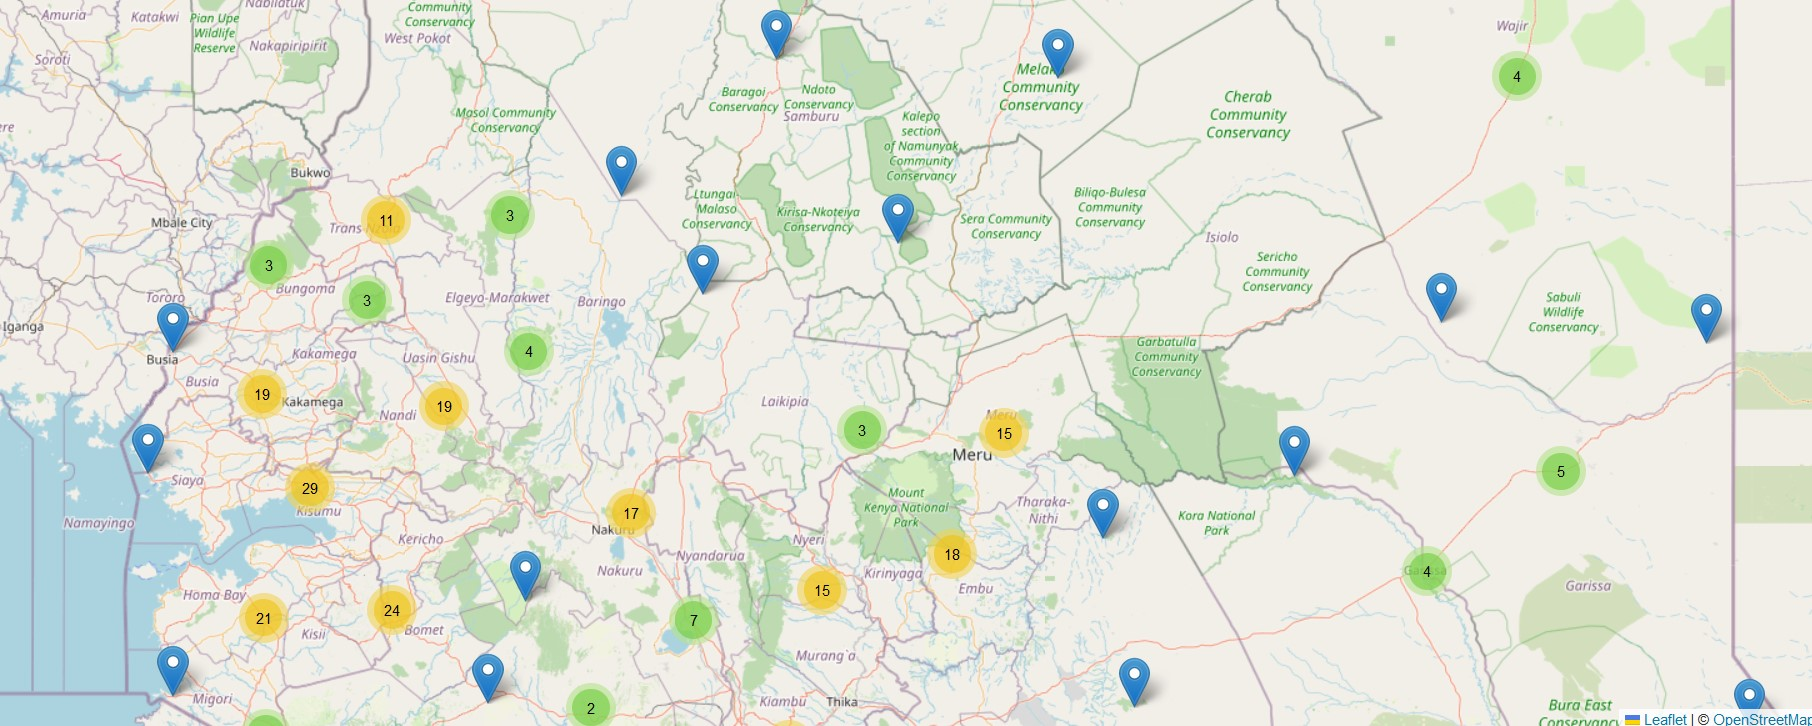
\includegraphics{../images/cluster-marker-plain.jpg}

Coming back full circle, circle markers are way better.

Most of the Ajax code was inspired by this \href{https://www.youtube.com/watch?v=R-V7XFUbrkw\&t=625s}{video}.

But wait! Hold your horses, there is a bug. Try to click on any of the spiderfied or lone hospitals and you will notice something that will raise eyebrows. All hospitals display the following popup when clicked:

\begin{verbatim}
Facility Name: Wajir Tb Manyatta Sub - District Hospital
Type: Sub-District Hospital
\end{verbatim}

\begin{Shaded}
\begin{Highlighting}[]
\NormalTok{knitr}\SpecialCharTok{::}\FunctionTok{include\_graphics}\NormalTok{(}\FunctionTok{rep}\NormalTok{(}\StringTok{\textquotesingle{}D:/gachuhi/my{-}leaflet/images/cluster{-}marker{-}bug.jpg\textquotesingle{}}\NormalTok{))}
\end{Highlighting}
\end{Shaded}

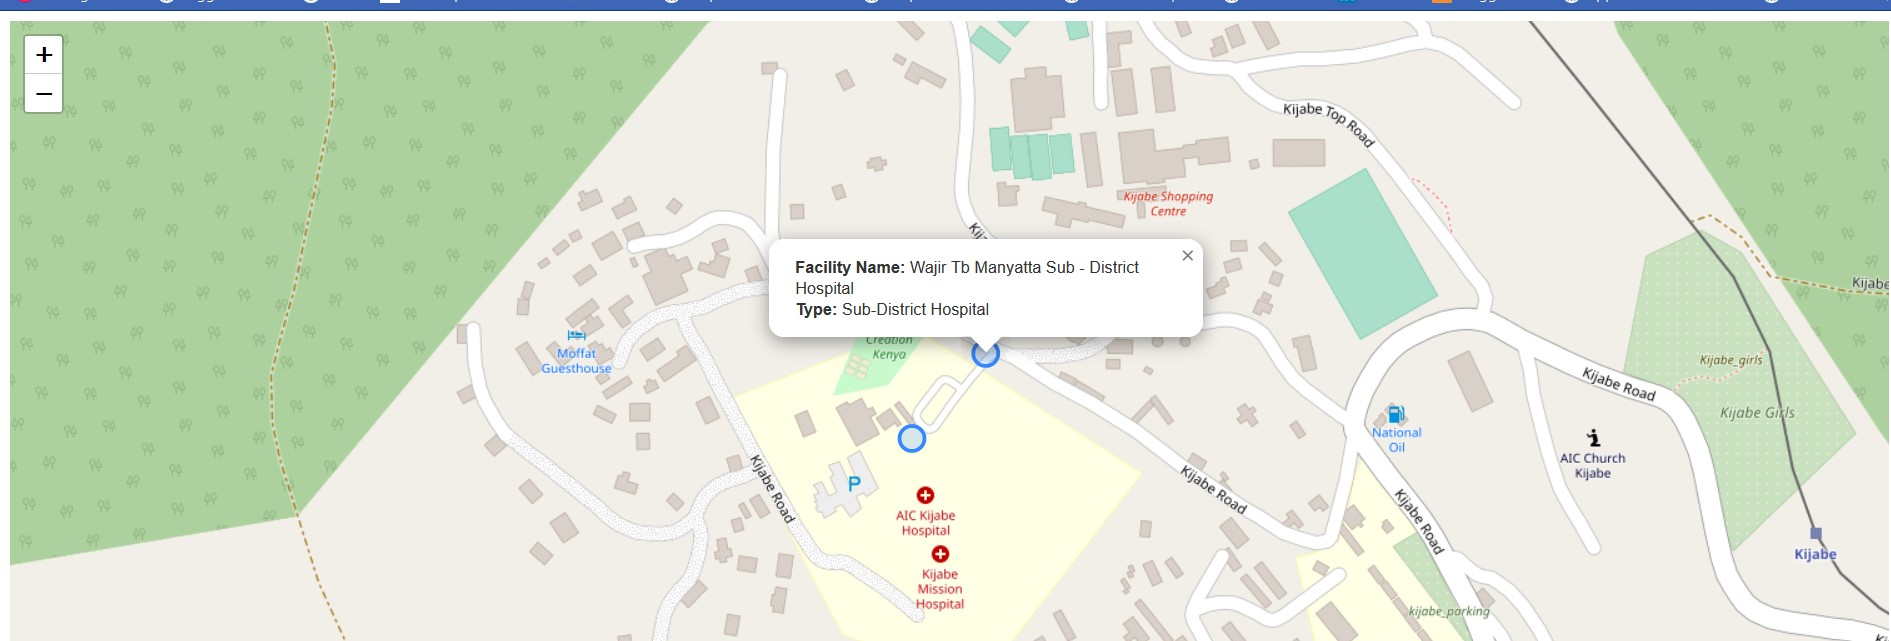
\includegraphics{../images/cluster-marker-bug.jpg}

Unless a developer would like to be left with an egg on the face for assigning the same place names to all hospitals, this should be dealt with expeditiously. Our code is alright, since it works in other scenarios such as \href{https://gis.stackexchange.com/questions/346104/popup-with-leaflet-markercluster-in-leaflet-map?utm_source=pocket_reader}{here}. However, it is unnacceptable to assign wrong place names in the world wide web.

Time to try a different strategy: using \texttt{fetch} API. We have worked with \texttt{fetch} before so we will not explain it that much here. Feel free to google about it as a refresher. Comment out the earlier code beginning from \texttt{var\ markers} to \texttt{map.addLayer(markers)} and replace it with the following code chunk.

\begin{verbatim}
fetch(url)
    .then((response) =>{
        return response.json()
    })
    .then((data) => {
        var markers = L.markerClusterGroup();

        var geojsonGroup = L.geoJSON(data, {
            onEachFeature : function(feature, layer){
                layer.bindPopup(`<b>Facility Name:</b> ${feature.properties.Facility_N} <br>
                <b>Type:</b> ${feature.properties.Type}`);
            },
            pointToLayer: function (feature, latlng) {
                return L.circleMarker(latlng);
            }
        });

        markers.addLayer(geojsonGroup);
        map.addLayer(markers);

    })
    .catch((error) => {
        console.log(`This is the error: ${error}`)
    })
\end{verbatim}

\begin{Shaded}
\begin{Highlighting}[]
\NormalTok{knitr}\SpecialCharTok{::}\FunctionTok{include\_graphics}\NormalTok{(}\FunctionTok{rep}\NormalTok{(}\StringTok{\textquotesingle{}D:/gachuhi/my{-}leaflet/images/cluster{-}marker{-}map{-}fixed.jpg\textquotesingle{}}\NormalTok{))}
\end{Highlighting}
\end{Shaded}

\includegraphics{../images/cluster-marker-map-fixed.jpg}

Now all points have their rightful and respective names.

\hypertarget{additional-features-of-cluster-marker-plugin}{%
\section{Additional features of Cluster marker plugin}\label{additional-features-of-cluster-marker-plugin}}

The official documentation of the plugin lists many other features that come along with the tool. We can't go through all of them but let's surmise just one important functionality: the \texttt{mouseover} event. A \texttt{mouseover} event triggers an action when a mouse hovers of a feature in Leaflet.

Let's demonstrate adding a hover event to our cluster marker map, thanks to this \href{https://gnisitricks.de/2019/03/Adding-Click-and-Mouseover-Events-simultaneously-to-GeoJson-Markers-on-a-Leaflet-Map/}{answer}.

\begin{verbatim}
/////// Added `mouseover` event

fetch(url)
    .then((response) =>{
        return response.json()
    })
    .then((data) => {
        var markers = L.markerClusterGroup({chunkedLoading: true}); // Splits the add layers to small intervals to prevent page freezing

        var geojsonGroup = L.geoJSON(data, {
            onEachFeature : function(feature, layer){
                layer.bindPopup(`<b>Facility Name:</b> ${feature.properties.Facility_N} <br>
                <b>Type:</b> ${feature.properties.Type}`);
            },
            pointToLayer: function (feature, latlng) {
                return L.circleMarker(latlng).on('mouseover', function(){
                    this.bindPopup(`Nearest_Center: ${feature.properties.Nearest_To}`).openPopup(); // Add mouseover event
                });
            }
        });

        markers.addLayer(geojsonGroup);
        map.addLayer(markers);

    })
    .catch((error) => {
        console.log(`This is the error: ${error}`)
    })
\end{verbatim}

From the above code, we added the \texttt{mouseover} event to each marker point using the \texttt{on} method. The \texttt{this} keyword in \texttt{this.bindPopup()} ties popups of selected variables to coordinates in the \texttt{var\ geojsonGroup} variable. We also sped the rendering of our Leaflet map by adding \texttt{chunkedLoading:\ true} parameter to \texttt{L.markerCluster()} function.

Hovering over each marker point will show a value of the \texttt{Nearest\_To} attribute which is an actual town centre in closest proximity to the hospital marker.

\begin{Shaded}
\begin{Highlighting}[]
\NormalTok{knitr}\SpecialCharTok{::}\FunctionTok{include\_graphics}\NormalTok{(}\FunctionTok{rep}\NormalTok{(}\StringTok{\textquotesingle{}D:/gachuhi/my{-}leaflet/images/cluster{-}marker{-}mouseover.jpg\textquotesingle{}}\NormalTok{))}
\end{Highlighting}
\end{Shaded}

\includegraphics{../images/cluster-marker-mouseover.jpg}

The code files used for this chapter are available from \href{https://github.com/sammigachuhi/my-leaflet-project/tree/main/my-leaflet-code/chapter-10-Cluster_marker_points}{here}.

\hypertarget{summary-8}{%
\section{Summary}\label{summary-8}}

Cluster marker points are a neat way of displaying several points. Upon zooming out, the spatially sparsed points coalesce to a single unit displaying a figure standing for the number of markers it holds. Upon zooming in, the points spiderfy, (think of spreading out) to their appropriate locations. Here are the lessons from this chapter.

\begin{itemize}
\item
  Clustering points is at times useful for map neatness. In Leaflet, this is made possible with the \texttt{Leaflet.markercluster} plugin.
\item
  It is possible to customize how the spiderfied marker points will appear. For example, instead of settling for the default styles of individual markers, we used the circle markers to show individual points.
\item
  It is also possible to add events to the spiderfied marker points. When clicked, the spiderfied marker points can show a popup, or trigger any other event as specified in its code block.
\end{itemize}

\hypertarget{mobile-friendly-webapps}{%
\chapter{Mobile Friendly Webapps}\label{mobile-friendly-webapps}}

\hypertarget{the-need-for-mobile-friendly-web-apps}{%
\section{The need for mobile friendly web apps}\label{the-need-for-mobile-friendly-web-apps}}

Short story. Not too long ago I was the proud owner of a famous phone brand on the decline. One time, when taking a photo of the iconic Ngong Hills for \href{https://www.wikilovesafrica.net/wikipedias-photographic-competition-focuses-on-africas-climate-weather/}{Wikipedia's Africa Climate photo contest}, the phone just died. That was it. A quick visit to the authorized dealer was greeted with the unbelievable and bemusing words of, ``We no longer ship the motherboard to the country anymore.'' Some healing has taken place, but I was totally heartbroken, and occassionaly suffer some nostalgia of the `good times' I had with my phone.

Now back to business. Webapps can be heavy, and they can load slowly on smaller devices such as smartphones. Apps that load slow can put off your web app users, so it is prudent to customize your webapp for your user's phones.

For this chapter, we will work on making our cluster marker app mobile friendly. We shall also add other functionalities to make the web app `heavier' in order to test to destruction if our ambitions of making our app load faster have worked.

In order to create a mobile friendly Leaflet experience, insert the below code within the \texttt{\textless{}head\textgreater{}} element of your \texttt{map.html}. The below \texttt{meta} tag tells the browser to disable unwanted scaling of the page and instead set it to its actual size.

\begin{verbatim}
<meta name="viewport" content="width=device-width, initial-scale=1.0, maximum-scale=1.0, user-scalable=no" />
\end{verbatim}

\hypertarget{the-basemaps}{%
\section{The basemaps}\label{the-basemaps}}

If you have gone through \protect\hyperlink{layer-groups-and-controls}{Chapter 8} where we created controls, the following will look familiar. We will add some basemaps and later on create their control widgets.

\begin{verbatim}
// Basemaps
var osm = L.tileLayer('https://tile.openstreetmap.org/{z}/{x}/{y}.png', {
    maxZoom: 19,
    attribution: '&copy; <a href="http://www.openstreetmap.org/copyright">OpenStreetMap</a>'
});

var cyclOSM = L.tileLayer('https://{s}.tile-cyclosm.openstreetmap.fr/cyclosm/{z}/{x}/{y}.png', {
    maxZoom: 20,
    attribution: '<a href="https://github.com/cyclosm/cyclosm-cartocss-style/releases" title="CyclOSM - Open Bicycle render">CyclOSM</a> | Map data: &copy; <a href="https://www.openstreetmap.org/copyright">OpenStreetMap</a> contributors'
}); // the CyclOSM tile layer available from Leaflet servers
\end{verbatim}

Let's add our basemaps to Leaflet.

\begin{verbatim}
// Add the Leaflet basemaps
var map = L.map('myMap', {
    layers: [osm, cyclOSM]
}).setView([-1.295287148, 36.81984753], 7);
\end{verbatim}

\hypertarget{adding-the-features}{%
\section{Adding the features}\label{adding-the-features}}

Remember our hospital json layer? Let's call it again and transform it to a cluster marker with \texttt{fetch}.

\begin{verbatim}
// Add hospital dataset

url = 'https://raw.githubusercontent.com/sammigachuhi/geojson_files/main/selected_hospitals.json'

var cluster = fetch(url)
    .then((response) =>{
        return response.json()
    })
    .then((data) => {
        var markers = L.markerClusterGroup();

        var geojsonGroup = L.geoJSON(data, {
            onEachFeature : function(feature, layer){
                var popupContent =  `<b>Facility Name:</b> ${feature.properties.Facility_N} <br>
                <b>Type:</b> ${feature.properties.Type}`;
                layer.bindPopup(popupContent)
            },
            pointToLayer: function (feature, latlng) {
                return L.circleMarker(latlng);
            }
        });

        markers.addLayer(geojsonGroup);
        map.addLayer(markers);

    })
    .catch((error) => {
        console.log(`This is the error: ${error}`)
    })
\end{verbatim}

Why was the \texttt{fetch} code being parsed to \texttt{var\ cluster}? Well, we were aiming for the stars. We wanted to have a layer control for our \texttt{cluster} variable too but unfortunately this plan failed.

Let's put our \texttt{basemaps} and \texttt{cluster} variables into JavaScript objects in order to create a layer control for each.

\begin{verbatim}
// Set object for the basemaps
var basemaps = {
    "OpenStreetMap": osm,
    'cycleOsm': cyclOSM,
}

////Don't add the 'overlays' object. For demonstration purposes only
// Set object for the overlay maps
var overlays = {
    'Hospitals': cluster
}
\end{verbatim}

Before you head on any further, inserting the \texttt{overlays} object into the \texttt{L.control.layers()} class results in several errors. This is why we were unable to create a control for the markers held in \texttt{var\ cluster}. The image below shows the errors appearing in the console after inserting the \texttt{overlays} object into \texttt{L.control.layers()}.

\begin{Shaded}
\begin{Highlighting}[]
\NormalTok{knitr}\SpecialCharTok{::}\FunctionTok{include\_graphics}\NormalTok{(}\FunctionTok{rep}\NormalTok{(}\StringTok{\textquotesingle{}D:/gachuhi/my{-}leaflet/images/mobile{-}friendly{-}error.jpg\textquotesingle{}}\NormalTok{))}
\end{Highlighting}
\end{Shaded}

\includegraphics{../images/mobile-friendly-error.jpg}

To get rid of the error showcased above, just comment out the \texttt{overlays} object and remove it from \texttt{L.control.layers()}. The \texttt{L.control.layers()} class should only contain the \texttt{basemap} object.

\hypertarget{zooming-to-the-mobile-users-location}{%
\section{Zooming to the mobile user's location}\label{zooming-to-the-mobile-users-location}}

According to the Leaflet official documentation, Leaflet has a handy shortcut of zooming in to the user's location. If for some reason it will not pinpoint the exact coordinates, it will create a buffer around the mobile user's approximate location.

\begin{verbatim}
// Zoom to your location
map.locate({setView: true, maxZoom: 16});
\end{verbatim}

\hypertarget{add-marker-to-mobile-users-geolocation}{%
\section{Add marker to mobile user's geolocation}\label{add-marker-to-mobile-users-geolocation}}

Even if the location is off by a couple of miles, at least a marker to show the triangulated position will help. At least you will not be \emph{all over} the map! The following code adds a marker to the mobile user's triangulated Latitude-Longitude coordinates, and displays a message showing the radius in which the mobile user is most likely to be found from the marker point.

\begin{verbatim}
// Add marker at your location
function onLocationFound(e) {
    var radius = e.accuracy;

    L.marker(e.latlng).addTo(map)
        .bindPopup("You are within " + Number((radius/1000).toFixed(2)) + " kilometers from this point").openPopup();

    L.circle(e.latlng, radius).addTo(map);
}
\end{verbatim}

Incase you forgot, the \texttt{on} method adds listeners. As a gentle reminder, listeners are codes that run when an event is triggered, such as the simple hovering of a mouse over a feature. In the below code, the listener \texttt{\textquotesingle{}locationfound\textquotesingle{}} triggers the \texttt{onLocationFound} function in case Leaflet successfully approximated the user's location.

\begin{verbatim}
map.on('locationfound', onLocationFound);
\end{verbatim}

The \texttt{locationfound} listener is responsible for the message bounded in red below when a browser loads a Leaflet map. Clicking \textbf{Allow} will give the browser the heads up to zoom to the user's location as it best can.

\begin{Shaded}
\begin{Highlighting}[]
\NormalTok{knitr}\SpecialCharTok{::}\FunctionTok{include\_graphics}\NormalTok{(}\FunctionTok{rep}\NormalTok{(}\StringTok{\textquotesingle{}D:/gachuhi/my{-}leaflet/images/location{-}found.jpg\textquotesingle{}}\NormalTok{))}
\end{Highlighting}
\end{Shaded}

\includegraphics{../images/location-found.jpg}

What if, getting the mobile user's geolocation is unsuccessful? We will create a function that outputs the error event to our console, as shown below.

\begin{verbatim}
// Error displayed after finding location failed
function onLocationError(e) {
    alert(e.message);
}
\end{verbatim}

Actually, \texttt{message} is an error event that displays the error message of a parameter. The \texttt{message} event is parsed to the \texttt{onLocationError} function. If the browser fails to approximate the user's location, the \texttt{onLocationError} function returns `true' which triggers an error alert on the browser.

\begin{verbatim}
map.on('locationerror', onLocationError);
\end{verbatim}

\hypertarget{the-mobile-webmap-app}{%
\section{The mobile webmap app}\label{the-mobile-webmap-app}}

Yours truly has saved you the hustle of detailing how this chapter's files have been saved to Github and subsequently converted to a webpage. The key thing to note is that the HTML file has to be named as \texttt{index.html} and not any other name such as \texttt{map.html} since the name `index' is the easiest way to render a file on the fly on Github. Some additional steps exist to launch our Leaflet map to the global web but to ensure brevity in this chapter, we suggest you visit this authoritative \href{https://docs.github.com/en/pages/getting-started-with-github-pages/creating-a-github-pages-site}{Github page} for further guidance. The link below should nevertheless allow you to view the webapp on your phone.

\url{https://sammigachuhi.github.io/hospitals_webapp/}

\begin{Shaded}
\begin{Highlighting}[]
\NormalTok{knitr}\SpecialCharTok{::}\FunctionTok{include\_graphics}\NormalTok{(}\FunctionTok{rep}\NormalTok{(}\StringTok{\textquotesingle{}D:/gachuhi/my{-}leaflet/images/mobile{-}app.jpg\textquotesingle{}}\NormalTok{))}
\end{Highlighting}
\end{Shaded}

\includegraphics{../images/mobile-app.jpg}

We had initially aimed for the stars by wanting to create a web app that in addition to the basemap layers, it would also feature some layer controls. However, it seemed like we landed on the skies instead. Nevertheless, this looks like a good hospital locations app. The sky is only the baseline for what further features can be built on top of this app.

The full code script is available from \href{https://github.com/sammigachuhi/my-leaflet-project/tree/main/my-leaflet-code/chapter-11-mobile-friendly-webapps}{here}.

\hypertarget{summary-9}{%
\section{Summary}\label{summary-9}}

Enabling a Leaflet map to be mobile friendly allows the Leaflet map to load fast as well as scale efficiently on a smartphone. Here is what you've learnt.

\begin{itemize}
\item
  A special \texttt{meta} tag is inserted in the \texttt{\textless{}head\textgreater{}} element of your HTML file to enable the browser scale smoothly when a user is viewing a Leaflet map on a smartphone.
\item
  Leaflet has a special function, the \texttt{map.locate} that geolocates and zooms to the user's exact coordinates. If for some reason precision fails, it creates a buffer around the mobile user's approximate location.
\item
  In case Leaflet is unable to approximate the user's location, one can resort to the \texttt{message} event which throws back an error on the browser.
\end{itemize}

\hypertarget{web-map-service-layers}{%
\chapter{Web Map Service Layers}\label{web-map-service-layers}}

\hypertarget{what-are-web-map-service-wms-layers}{%
\section{What are Web Map Service (WMS) Layers?}\label{what-are-web-map-service-wms-layers}}

A \href{https://gisgeography.com/web-mapping-services-wms/}{Web Mapping Service (WMS)} consists of geospatial data hosted through the internet with standards set by the Open Geospatial Consortium (OGS).

A WMS enables the exchange of spatial information and viewing over the web in the form of a map or image to your browser. The most common formats of Web Mapping Services are Web Map Services (WMS), Web Feature Services (WFS), Web Coverage Services (WCS), Web Processing Services (WPS), Web Map Tile Services (WMTS), and Web Coverage Processing Services (WCPS). However, the Web Map Services (WMS) layer is the most used. It offers basic panning, zooming and quick rendering speeds.

\hypertarget{loading-a-wms-server}{%
\section{Loading a WMS server}\label{loading-a-wms-server}}

To load a WMS layer into Leaflet, we use the \texttt{L.tileLayer.wms} class. As simple as that. So let's set up our Leaflet map. Create a new JavaScript file named \texttt{wms\_layers.js} and insert the following code:

\begin{verbatim}
let map = L.map('myMap').setView([-1.295287148, 36.81984753], 7);

let tileLayer = L.tileLayer('https://tile.openstreetmap.org/{z}/{x}/{y}.png', {
    maxZoom: 19,
    attribution: '&copy; <a href="http://www.openstreetmap.org/copyright">OpenStreetMap</a>'
});
\end{verbatim}

We have added an OSM layer because we want to create a layer control widget that also contains WMS layers so that you can switch between an Open Street Map (OSM) layer and a WMS. For this exercise, we shall add two WMS layers.

\begin{verbatim}
let wmsLayerTopo = L.tileLayer.wms('https://www.gmrt.org/services/mapserver/wms_merc_mask?', {
    layers: 'topo',
    format: 'image/png'
})

let wmsLayerTopomask = L.tileLayer.wms('https://www.gmrt.org/services/mapserver/wms_merc_mask?', {
    layers: 'topo-mask',
    format: 'image/png'
})
\end{verbatim}

\hypertarget{adding-wms-to-layer-control}{%
\section{Adding WMS to layer control}\label{adding-wms-to-layer-control}}

Let's insert the above web map layers into a JavaScript object before parsing it to a layer control.

\begin{verbatim}
var basemaps = {
    OSM: tileLayer,
    Topo: wmsLayerTopo,
    Topo_mask: wmsLayerTopomask,
}
\end{verbatim}

Now let's parse the object into a control. If you did \protect\hyperlink{layer-groups-and-controls}{Chapter 8} then this should look familiar.

\begin{verbatim}
L.control.layers(basemaps).addTo(map);

basemaps.Topo.addTo(map);  // To have the Topo as the default map layer
\end{verbatim}

The last line \texttt{basemaps.Topo.addTo(map)} serves to set up the default layer that will appear when the map is loaded. In this case it is the \texttt{Topo} key in \texttt{var\ basemaps}. If this last line is omitted, Leaflet will only show a blank canvas unless one of the radioitems is selected.

\begin{Shaded}
\begin{Highlighting}[]
\NormalTok{knitr}\SpecialCharTok{::}\FunctionTok{include\_graphics}\NormalTok{(}\FunctionTok{rep}\NormalTok{(}\StringTok{\textquotesingle{}D:/gachuhi/my{-}leaflet/images/wms\_layer.jpg\textquotesingle{}}\NormalTok{))}
\end{Highlighting}
\end{Shaded}

\includegraphics{../images/wms_layer.jpg}

And that's it!

Even though we wanted to work with African-based WMS layers, of which \href{https://training.digitalearthafrica.org/en/latest/OWS_tutorial.html}{Digital Earth Africa} provides plenty of them, for some reason this was not possible despite diligently following their documentation. It is quite ironic that they can be easily loaded in Qgis and not Leaflet.

Interested in getting other WMS layers? Go to \href{https://directory.spatineo.com/}{Spartineo.com}.

The files used in this chapter are available \href{https://github.com/sammigachuhi/my-leaflet-project/tree/main/my-leaflet-code/chapter-12-Web_map_service_layers}{here}.

\hypertarget{summary-10}{%
\section{Summary}\label{summary-10}}

A Web Mapping Service (WMS) layer in many respects looks and acts like a basemap. Just like Open Street Map and other similar servers, WMS layers host data through the internet. Here are the take homes from this chapter.

\begin{itemize}
\item
  A Web Mapping Service consists of geospatial data hosted through the internet with standards set by the Open Geospatial Consortium (OGS).
\item
  The most common formats of Web Mapping Services are Web Map Services (WMS), Web Feature Services (WFS), Web Coverage Services (WCS), Web Processing Services (WPS), Web Map Tile Services (WMTS), and Web Coverage Processing Services (WCPS).
\item
  The \texttt{L.tileLayer.wms} class is used to load WMS layers into Leaflet.
\item
  Just like any other basemap, one can parse WMS layer into Leaflet controls, as seen with \texttt{wmsLayerTopo} and \texttt{wmsLayerTopomask}.
\end{itemize}

\hypertarget{standard-website-with-leaflet-project}{%
\chapter{Standard Website with Leaflet Project}\label{standard-website-with-leaflet-project}}

\hypertarget{get-the-html-template}{%
\section{Get the HTML Template}\label{get-the-html-template}}

Back in \protect\hyperlink{embedding-leaflet-map-to-an-external-website}{Chapter 4} we inserted a Leaflet map into a pale looking website. Taking that exercises a little further, we would like to demonstrate how Leaflet can be added to a standard, professional looking HTML website. This chapter will train you how to insert a Leaflet map into your company's, client's or even colleague's website.

The template used in this exercise was acquired from \href{https://www.free-css.com/free-css-templates}{Free CSS.com} and is available \href{https://www.free-css.com/assets/files/free-css-templates/download/page291/elearning.zip}{here}. Extract the files and take a look at the HTML documents. That is, the \texttt{index.html}, \texttt{about.html}, \texttt{contact.html}, \texttt{courses.html}, \texttt{team.html} and \texttt{testimonial.html} files. Pay special attention to the \texttt{\textless{}head\textgreater{}} element and the \texttt{\textless{}div\textgreater{}} containing the Gallery section of the website. The Gallery \texttt{\textless{}div\textgreater{}} looks like so:

\begin{verbatim}
<div class="col-lg-3 col-md-6">
                    <h4 class="text-white mb-3">Gallery</h4>
                    <div class="row g-2 pt-2">
                        <div class="col-4">
                            <img class="img-fluid bg-light p-1" src="img/course-1.jpg" alt="">
                        </div>
                        <div class="col-4">
                            <img class="img-fluid bg-light p-1" src="img/course-2.jpg" alt="">
                        </div>
                        <div class="col-4">
                            <img class="img-fluid bg-light p-1" src="img/course-3.jpg" alt="">
                        </div>
                        <div class="col-4">
                            <img class="img-fluid bg-light p-1" src="img/course-2.jpg" alt="">
                        </div>
                        <div class="col-4">
                            <img class="img-fluid bg-light p-1" src="img/course-3.jpg" alt="">
                        </div>
                        <div class="col-4">
                            <img class="img-fluid bg-light p-1" src="img/course-1.jpg" alt="">
                        </div>
                    </div>
                </div>
\end{verbatim}

Here is where the Gallery in the eLearning webpage is situated (bounded in red).

\begin{Shaded}
\begin{Highlighting}[]
\NormalTok{knitr}\SpecialCharTok{::}\FunctionTok{include\_graphics}\NormalTok{(}\FunctionTok{rep}\NormalTok{(}\StringTok{\textquotesingle{}D:/gachuhi/my{-}leaflet/images/gallery.jpg\textquotesingle{}}\NormalTok{))}
\end{Highlighting}
\end{Shaded}

\includegraphics{../images/gallery.jpg}

Why do we want to change the gallery, or rather, to insert a Leaflet map in its place? It seemed a good idea to replace the pretty looking pictures with a webmap since this website is for demonstration purposes only.

\hypertarget{embed-leaflet-to-standard-html-website}{%
\section{Embed Leaflet to standard html website}\label{embed-leaflet-to-standard-html-website}}

Since we want to integrate a Leaflet map to the eLearning website, we will have to load the requisite Leaflet links and scripts to the eLearning dummy website's \texttt{\textless{}head\textgreater{}} element, just like we used to do to our \texttt{map.html}. Thereafter, we shall replace the entire gallery section with just one \texttt{\textless{}div\textgreater{}} that references one of our many Leaflet JavaScript files.

Ready? Let's go.

Assuming you are working on VSCode, copy all the plugin files for Leaflet, such as the \texttt{Leaflet.markercluster-master} folder and all the others you have extracted at one point or another in previous chapters. The names of these folders are enclosed with a red border in the image below.

\begin{Shaded}
\begin{Highlighting}[]
\NormalTok{knitr}\SpecialCharTok{::}\FunctionTok{include\_graphics}\NormalTok{(}\FunctionTok{rep}\NormalTok{(}\StringTok{\textquotesingle{}D:/gachuhi/my{-}leaflet/images/elearning{-}plugins.jpg\textquotesingle{}}\NormalTok{))}
\end{Highlighting}
\end{Shaded}

\includegraphics{../images/elearning-plugins.jpg}

Why are we ensuring that the Leaflet plugin folders are in the same directory as our eLearning template files? It is because we want to avoid the need of tinkering with the relative path, which has to change if the (plugin) folders were located in a different directory from that of our eLearning website.

Go to the \texttt{index.html} file of your eLearning template. From the \texttt{\textless{}head\textgreater{}} to \texttt{\textless{}/head\textgreater{}} tags, replace the existing code with the following:

\begin{verbatim}
<meta charset="utf-8">
    <!-- For leaflet and mobile compatibility -->
    <meta name="viewport" content="width=device-width, initial-scale=1.0, maximum-scale=1.0, user-scalable=no" />

    <title>eLEARNING - eLearning HTML Template</title>
    <meta content="width=device-width, initial-scale=1.0" name="viewport">
    <meta content="" name="keywords">
    <meta content="" name="description">

    <!-- Favicon -->
    <link href="img/favicon.ico" rel="icon">

    <!-- Google Web Fonts -->
    <link rel="preconnect" href="https://fonts.googleapis.com">
    <link rel="preconnect" href="https://fonts.gstatic.com" crossorigin>
    <link href="https://fonts.googleapis.com/css2?family=Heebo:wght@400;500;600&family=Nunito:wght@600;700;800&display=swap" rel="stylesheet">

    <!-- Icon Font Stylesheet -->
    <link href="https://cdnjs.cloudflare.com/ajax/libs/font-awesome/5.10.0/css/all.min.css" rel="stylesheet">
    <link href="https://cdn.jsdelivr.net/npm/bootstrap-icons@1.4.1/font/bootstrap-icons.css" rel="stylesheet">

    <!-- Libraries Stylesheet -->
    <link href="lib/animate/animate.min.css" rel="stylesheet">
    <link href="lib/owlcarousel/assets/owl.carousel.min.css" rel="stylesheet">

    <!-- Customized Bootstrap Stylesheet -->
    <link href="css/bootstrap.min.css" rel="stylesheet">

    <!-- Template Stylesheet -->
    <link href="css/style.css" rel="stylesheet">

    <!-- For leaflet -->
    <link rel="stylesheet" href="https://unpkg.com/leaflet@1.9.3/dist/leaflet.css"
        integrity="sha256-kLaT2GOSpHechhsozzB+flnD+zUyjE2LlfWPgU04xyI="
        crossorigin=""/>
    <link rel="stylesheet" href="Leaflet.Control.Opacity-master\Leaflet.Control.Opacity-master\dist\L.Control.Opacity.css">
    <!-- For Leaflet marker clusters -->
    <link rel="stylesheet" href="Leaflet.markercluster-master\Leaflet.markercluster-master\dist\MarkerCluster.Default.css">  

    <!-- For leaflet scripts -->
    <script src="https://unpkg.com/leaflet@1.9.3/dist/leaflet.js"
        integrity="sha256-WBkoXOwTeyKclOHuWtc+i2uENFpDZ9YPdf5Hf+D7ewM="
        crossorigin=""></script>
    <script src="leaflet-ajax-gh-pages\dist\leaflet.ajax.js"></script>
    <script src="leaflet-ajax-gh-pages\dist\leaflet.ajax.min.js"></script>
    <script src="leaflet-ajax-gh-pages\example\leaflet.spin.js"></script>
    <script src="leaflet-ajax-gh-pages\example\spin.js"></script> 
    <script src="Leaflet.heat-gh-pages\Leaflet.heat-gh-pages\dist\leaflet-heat.js"></script>
    <script src="https://ajax.googleapis.com/ajax/libs/jquery/2.1.4/jquery.min.js"></script>
    <!-- For leaflet cluster markers -->
    <script src="Leaflet.markercluster-1.4.1\Leaflet.markercluster-1.4.1\dist\leaflet.markercluster.js"></script>
    <script src="Leaflet.markercluster-1.4.1\Leaflet.markercluster-1.4.1\dist\leaflet.markercluster-src.js"></script>
    
\end{verbatim}

The first alteration we will do to our eLearning website's HTML folder is to add the relevant Leaflet \texttt{\textless{}link\textgreater{}} and \texttt{\textless{}script\textgreater{}} tags. These \texttt{\textless{}link\textgreater{}} and \texttt{\textless{}script\textgreater{}} tags have just been copy pasted from the \texttt{map.html} file we have been dealing with so far.

Now that we have the requisite \texttt{\textless{}link\textgreater{}} and \texttt{\textless{}script\textgreater{}} tags to embed Leaflet into our eLeaflet demo website, we only need to insert the path to our JavaScript file containing the Leaflet code. The JavaScript is of course responsible for firing up the Leaflet map in our eLearning website. For this exercise, we shall use the \texttt{cluster\_markers.js} file we have had so much fun with. Copy paste this file into the same folder containing your eLeaflet website's folders.

Alright.

Time to add the leaflet map. Where? At the gallery section.

As a reminder, it looks like this:

\begin{verbatim}
<div class="col-lg-3 col-md-6">
                    <h4 class="text-white mb-3">Gallery</h4>
                    <div class="row g-2 pt-2">
                        <div class="col-4">
                            <img class="img-fluid bg-light p-1" src="img/course-1.jpg" alt="">
                        </div>
                        <div class="col-4">
                            <img class="img-fluid bg-light p-1" src="img/course-2.jpg" alt="">
                        </div>
                        <div class="col-4">
                            <img class="img-fluid bg-light p-1" src="img/course-3.jpg" alt="">
                        </div>
                        <div class="col-4">
                            <img class="img-fluid bg-light p-1" src="img/course-2.jpg" alt="">
                        </div>
                        <div class="col-4">
                            <img class="img-fluid bg-light p-1" src="img/course-3.jpg" alt="">
                        </div>
                        <div class="col-4">
                            <img class="img-fluid bg-light p-1" src="img/course-1.jpg" alt="">
                        </div>
                    </div>
                </div>
\end{verbatim}

You may have to scroll \emph{really} down to locate it. Right under the \texttt{\textless{}h4\ class="text-white\ mb-3"\textgreater{}Gallery\textless{}/h4\textgreater{}} tag, replace it with the following code, all the way to the \texttt{\textless{}div\textgreater{}} tag after \texttt{\textless{}img\ class="img-fluid\ bg-light\ p-1"\ src="img/course-1.jpg"\ alt=""\textgreater{}}.

\begin{verbatim}
<div id="myMap"> 
                        <script src="cluster-markers.js">

                        </script>
                    </div>
\end{verbatim}

Perhaps an image will clarify matters a bit. This is where you are to insert the path to your \texttt{cluster-markers.js} file.

\begin{Shaded}
\begin{Highlighting}[]
\NormalTok{knitr}\SpecialCharTok{::}\FunctionTok{include\_graphics}\NormalTok{(}\FunctionTok{rep}\NormalTok{(}\StringTok{\textquotesingle{}D:/gachuhi/my{-}leaflet/images/div\_replace.jpg\textquotesingle{}}\NormalTok{))}
\end{Highlighting}
\end{Shaded}

\includegraphics{../images/div_replace.jpg}

Also as a heads up, remember to replace the \texttt{\textless{}h4\textgreater{}} tags with the statement \texttt{Our\ Location}. It's no longer a gallery but a webmap!

As if that was not enough, we also have to set the CSS properties for our Leaflet map.

\hypertarget{editing-the-css}{%
\section{Editing the CSS}\label{editing-the-css}}

Open the \texttt{style.css} file of your eLearning template in your text editor (such as VS code). The path to the CSS file is as follows:

\begin{verbatim}
elearning-template\css\style.css
\end{verbatim}

Scroll down to the very bottom of \texttt{style.css} and paste the following CSS properties for our Leaflet map.

\begin{verbatim}
#myMap { 
    height: 400px;
    width: auto; 
}
\end{verbatim}

Remember the \texttt{\#} and the text that follows references the specific name of that \texttt{ID} attribute from the countless HTML tags in \texttt{index.html}. The above CSS selector references the \texttt{\textless{}div\textgreater{}} with the ID-- \texttt{\#myMap}.

After reloading \texttt{index.html}, this is how our Leaflet map looks inside the eLearning template.

\begin{Shaded}
\begin{Highlighting}[]
\NormalTok{knitr}\SpecialCharTok{::}\FunctionTok{include\_graphics}\NormalTok{(}\FunctionTok{rep}\NormalTok{(}\StringTok{\textquotesingle{}D:/gachuhi/my{-}leaflet/images/location\_elearning.jpg\textquotesingle{}}\NormalTok{))}
\end{Highlighting}
\end{Shaded}

\includegraphics{../images/location_elearning.jpg}

Good.

\hypertarget{embedding-leaflet-to-every-webpage}{%
\section{Embedding Leaflet to every webpage}\label{embedding-leaflet-to-every-webpage}}

Now click the \textbf{About}, \textbf{Courses}, \textbf{Pages/Our Team}, \textbf{Pages/Testimonial} and \textbf{Contact} web pages. Is the Leaflet map there in each case? No.~It's the same ol' gallery. Imagine you will have to replace the \texttt{\textless{}head\textgreater{}} and Gallery \texttt{\textless{}div\textgreater{}} elements of the respective \texttt{about.html}, \texttt{courses.html}, \texttt{team.html}, \texttt{testimonial.html} and \texttt{contact.html} webpages here as well with the relevant Leaflet paths! Luckily, since you have hopefully got the gist of it, the following link contains the eLearning folder with Leaflet map embedded in all the aforementioned webpages.

\href{https://github.com/sammigachuhi/my-leaflet-project/tree/main/elearning-template}{elearning\_template\_demo}

\hypertarget{posting-the-html-website-to-the-world}{%
\section{Posting the Html website to the world}\label{posting-the-html-website-to-the-world}}

This chapter will leave out the details of saving your files to Github. Nevertheless, as mentioned in \protect\hyperlink{mobile-friendly-webapps}{Chapter 11}, the name \texttt{index} in your HTML file is automatically considered the root HTML file by Github. With that said, here is the link to our eLearning website with a Leaflet webmap embedded therein.

\href{https://sammigachuhi.github.io/elearning_template_demo/}{eLearning website}

\hypertarget{summary-11}{%
\section{Summary}\label{summary-11}}

Having the necessary Leaflet folders in the same directory as your HTML website's files prevents the Leaflet map from failing to load due to a broken path. Here are other lesson's we have encountered.

\begin{itemize}
\item
  In order to embed a Leaflet map into your website, you have to load the requisite Leaflet \texttt{\textless{}link\textgreater{}} and \texttt{\textless{}script\textgreater{}} tags into your \texttt{\textless{}head\textgreater{}} and where necessary, \texttt{\textless{}div\textgreater{}} elements.
\item
  Insert the JavaScript code that fires up your Leaflet using the \texttt{\textless{}script\textgreater{}} tags. This was the method used to insert the JavaScript file \texttt{cluster-markers.js} into the eLeaflet dummy website.
\item
  It is also important to ensure your Leaflet map appears in the right place in all the child webpages. For example, Leaflet also had to be embedded in the webpages of \texttt{about.html}, \texttt{courses.html}, \texttt{team.html}, \texttt{testimonial.html} and \texttt{contact.html} at the Gallery section just as it was done for their parent file-- \texttt{index.html}.
\end{itemize}

\hypertarget{esri-and-leaflet}{%
\chapter{ESRI and Leaflet}\label{esri-and-leaflet}}

\hypertarget{an-overview-of-esri}{%
\section{An overview of ESRI}\label{an-overview-of-esri}}

Alright. If you are a GIS practitioner, you have probably heard about ESRI, one of the world's leading geospatial software and services provider. You (might) have also come across various ESRI basemap servers, such as ESRI topographic, ESRI streets and ESRI Imagery layers. They also have plugins that allow Leaflet users to access the ArcGIS functionalities. For example, the ESRI plugins for Leaflet allow you to access some ESRI basemaps and products, while also allowing you to become an ESRI ArcGIS JavaScript developer.

To use ESRI Leaflet, you have to create an \href{https://developers.arcgis.com/dashboard/}{ArcGIS Developer account} and also get an \href{https://developers.arcgis.com/esri-leaflet/authentication/create-an-api-key/}{API key}. Kindly do so before proceeding.

\hypertarget{esri-leaflet-plugins}{%
\section{ESRI Leaflet plugins}\label{esri-leaflet-plugins}}

As we had mentioned earlier, you need ESRI Leaflet plugins to experience all the ArcGIS functionalities possible with your Application Programming Interface (API) key. Remember your \texttt{map.html} file? To experience Leaflet in ESRI, add the following \texttt{\textless{}script\textgreater{}} tags to the \texttt{\textless{}head\textgreater{}} element of your \texttt{map.html} file.

\begin{verbatim}
<!-- Load Esri Leaflet from CDN -->
        <script src="https://unpkg.com/esri-leaflet@3.0.10/dist/esri-leaflet.js"></script>
        <script src="https://unpkg.com/esri-leaflet-vector@4.0.2/dist/esri-leaflet-vector.js"></script>
\end{verbatim}

Create a new JavaScript file called \texttt{esri\_leaflet.js} and get ready to enjoy ESRI services!

\hypertarget{creating-an-esri-leaflet-map}{%
\section{Creating an ESRI Leaflet map}\label{creating-an-esri-leaflet-map}}

On your blank \texttt{esri\_leaflet.js} file, create a variable to store your API Key. This key is important to access your ESRI benefits, much like the magic phrase ``Open Sesame'' which would open a doorway to a cave full of treasures in the legendary story of \emph{Ali Baba and the Forty Thieves}!

Below is an example of how to access your API key from your ArcGIS Developer account.

\begin{Shaded}
\begin{Highlighting}[]
\NormalTok{knitr}\SpecialCharTok{::}\FunctionTok{include\_graphics}\NormalTok{(}\FunctionTok{rep}\NormalTok{(}\StringTok{\textquotesingle{}D:/gachuhi/my{-}leaflet/images/esri\_leaflet\_api.jpg\textquotesingle{}}\NormalTok{))}
\end{Highlighting}
\end{Shaded}

\includegraphics{../images/esri_leaflet_api.jpg}

Copy paste that key to your \texttt{esri\_leaflet.js} file.

\begin{verbatim}
const apiKey = "Your key";
\end{verbatim}

Let's proceed to create a basemap. To create one, just create a variable called \texttt{basemapEnum} that stores the ESRI basemap identifier. In ESRI Leaflet, a basemap is called by parsing the provider name and the desired style, like so: \texttt{\{Provider\}:\{Style\ name\}} or
\texttt{\{Provider\}:\{Style\ name\}:\{Component\}}. In our case, we want the ArcGIS streets basemap layer.

\begin{verbatim}
const basemapEnum = "ArcGIS:Streets";
\end{verbatim}

Alright. It's about time we fired up our mapping power. Create an ESRI Leaflet map instance much like we have always been doing.

\begin{verbatim}
const map = L.map("myMap", {
    minZoom: 2
}).setView([0.3556, 37.5833], 6.5);
\end{verbatim}

We had created a basemap variable earlier, so we will parse it to the \texttt{L.esri.Vector.vectorBasemapLayer} class which is responsible for creating basemaps. Actually one can also parse the \texttt{\{Provider\}:\{Style\ name\}} to the \texttt{L.esri.vector.vectorBasemapLayer()} class but our method of using variable names looks cleaner.

\begin{verbatim}
L.esri.Vector.vectorBasemapLayer(basemapEnum, {
    apiKey: apiKey,
}).addTo(map);
\end{verbatim}

Now open your \texttt{map.html} file. It should look like below.

\begin{Shaded}
\begin{Highlighting}[]
\NormalTok{knitr}\SpecialCharTok{::}\FunctionTok{include\_graphics}\NormalTok{(}\FunctionTok{rep}\NormalTok{(}\StringTok{\textquotesingle{}D:/gachuhi/my{-}leaflet/images/esri\_leaflet\_basemap.jpg\textquotesingle{}}\NormalTok{))}
\end{Highlighting}
\end{Shaded}

\includegraphics{../images/esri_leaflet_basemap.jpg}

Now imagine there are other basemap styles as shown in this \href{https://developers.arcgis.com/documentation/mapping-apis-and-services/maps/services/basemap-layer-service/\#default-basemap-styles}{webpage}.

\hypertarget{geocode-search}{%
\section{Geocode search}\label{geocode-search}}

Of course there are other ESRI Leaflet functionalities. Out of curiousity, a brief search was made to find out an ESRI plugin that loads raster layers in the hope it would be simpler in operation compared to the \href{https://github.com/GeoTIFF/georaster-layer-for-leaflet}{georaster plugin of Leaflet}. Although both have a plugin for downloading \texttt{.jpeg} and \texttt{.png} image formats, none is good enough for loading geospatial raster files such as \texttt{.tiff}. Nevertheless, there are other cool services that ESRI Leaflet offers, such as geocode search\footnote{Geocoding is the process of converting address or place text into a location. The geocoding service provides address and place geocoding as well as reverse geocoding}.

For the rest of this chapter, we shall create a geocoding service using ESRI Leaflet.

\hypertarget{add-search-bar}{%
\section{Add search bar}\label{add-search-bar}}

Add the following \texttt{\textless{}link\textgreater{}} and \texttt{\textless{}script\textgreater{}} to your \texttt{\textless{}head\textgreater{}} element.

\begin{verbatim}
<!-- Load Esri Leaflet Geocoder from CDN -->
        <link rel="stylesheet" href="https://unpkg.com/esri-leaflet-geocoder@3.1.4/dist/esri-leaflet-geocoder.css">
        <script src="https://unpkg.com/esri-leaflet-geocoder@3.1.4/dist/esri-leaflet-geocoder.js"></script>
\end{verbatim}

We will first add a search control widget to the topright of our ESRI Leaflet map. Search control widgets are created using the \texttt{L.esri.Geocoding.geosearch} class. In the below code, we have parsed the \texttt{L.esri.Geocoding.geosearch} to the variable \texttt{searchControl}.

\begin{verbatim}
const searchControl = L.esri.Geocoding.geosearch({
        position: "topright",
        placeholder: "Enter an address or place e.g. 1 York St",
        useMapBounds: false,

      }).addTo(map);
\end{verbatim}

Just like in Leaflet, ESRI Leaflet constructors have their options. Please refer to the options for this specific constructor \href{https://developers.arcgis.com/esri-leaflet/api-reference/controls/geosearch/}{here}.

Another small thing; change your \texttt{const\ basemapEnum} to read \texttt{ArcGis:Navigation}.

\begin{verbatim}
const basemapEnum = "ArcGIS:Navigation";
\end{verbatim}

Upon refreshing your \texttt{map.html} file, apart from having a new basemap style, you will see a new search bar at the top right. However, it is non-functional. It takes us nowhere.

\begin{Shaded}
\begin{Highlighting}[]
\NormalTok{knitr}\SpecialCharTok{::}\FunctionTok{include\_graphics}\NormalTok{(}\FunctionTok{rep}\NormalTok{(}\StringTok{\textquotesingle{}D:/gachuhi/my{-}leaflet/images/search\_bar.jpg\textquotesingle{}}\NormalTok{))}
\end{Highlighting}
\end{Shaded}

\includegraphics{../images/search_bar.jpg}

\hypertarget{make-the-search-bar-functional}{%
\section{Make the search bar functional}\label{make-the-search-bar-functional}}

In order to make the search bar do what it says, we will set the value of the \texttt{providers} key to a \texttt{arcgisOnlineProvider}. The latter is instantiated with the constructor \texttt{L.esri.Geocoding.arcgisOnlineProvider}. ESRI has various open source tutorials on its \href{https://developers.arcgis.com/esri-leaflet/geocode-and-search/search-for-an-address/?utm_source=pocket_saves}{platform} that provide succinct and concise explanation for most of its tools.

\begin{verbatim}
const searchControl = L.esri.Geocoding.geosearch({
    position: "topright",
    placeholder: "Enter an address or place e.g. 1 York St",
    useMapBounds: false,

    // Add provider
    providers: [
        L.esri.Geocoding.arcgisOnlineProvider({
          apikey: apiKey,
          nearby: {
            lat: 0.3556,
            lng: 37.5833
          }
        })
      ]

  }).addTo(map);
  
\end{verbatim}

Now try your search bar again. Some location names appear as you type them in, and if you press \textbf{Enter} it takes you to the exact location. This is good except for one thing: there is no marker to pinpoint that specific address. The following section outlines how to enable ESRI create a marker on the fly at any searched location name.

\begin{Shaded}
\begin{Highlighting}[]
\NormalTok{knitr}\SpecialCharTok{::}\FunctionTok{include\_graphics}\NormalTok{(}\FunctionTok{rep}\NormalTok{(}\StringTok{\textquotesingle{}D:/gachuhi/my{-}leaflet/images/searchable.jpg\textquotesingle{}}\NormalTok{))}
\end{Highlighting}
\end{Shaded}

\includegraphics{../images/searchable.jpg}

\hypertarget{adding-an-auto-generated-location-pin}{%
\section{Adding an auto-generated location pin}\label{adding-an-auto-generated-location-pin}}

First add a layer group to store the geocoding results.

\begin{verbatim}
const results = L.layerGroup().addTo(map);
\end{verbatim}

We will create an event handler to access the \texttt{data} from the search results. We shall also add a \texttt{clearLayers} call to remove the previous data from the layer group. This is beginning to sound complicated, but if the reader desires further clarity, they should refer to the \href{https://developers.arcgis.com/esri-leaflet/geocode-and-search/search-for-an-address/?utm_source=pocket_saves}{ESRI Leaflet geocoding tutorial}.

\begin{verbatim}
searchControl.on("results", (data) => {
        results.clearLayers();

      });
      
\end{verbatim}

The following loop adds the coordinates of the searched location to the marker. This loop goes into the \texttt{searchControl} code block.

\begin{verbatim}
for (let i = data.results.length - 1; i >= 0; i--) {
          const marker = L.marker(data.results[i].latlng);

          results.addLayer(marker);

        }
\end{verbatim}

The \texttt{lngLatString} variable below will store the rounded coordinates, and our familiar \texttt{bindPopup} and \texttt{openPopup} will show the coordinates and our address.

\begin{verbatim}
const lngLatString = `${Math.round(data.results[i].latlng.lng * 100000) / 100000}, ${
            Math.round(data.results[i].latlng.lat * 100000) / 100000
          }`;
          marker.bindPopup(`<b>${lngLatString}</b><p>${data.results[i].properties.LongLabel}</p>`);

          results.addLayer(marker);

          marker.openPopup();
\end{verbatim}

The entire \texttt{searchControl} code block should look like below.

\begin{verbatim}
searchControl.on("results", (data) => {
    results.clearLayers();

    for (let i = data.results.length - 1; i >= 0; i--) {
        const marker = L.marker(data.results[i].latlng);

        const lngLatString = `${Math.round(data.results[i].latlng.lng * 100000) / 100000}, ${
            Math.round(data.results[i].latlng.lat * 100000) / 100000
          }`;
          marker.bindPopup(`<b>${lngLatString}</b><p>${data.results[i].properties.LongLabel}</p>`);

        results.addLayer(marker);

        marker.openPopup();

      }

  });
  
\end{verbatim}

So now when you search for a particular place in the search bar and press \textbf{Enter}, a marker and with a pop up showcasing the address and longitude-latitude coordinates of the location should appear.

\begin{Shaded}
\begin{Highlighting}[]
\NormalTok{knitr}\SpecialCharTok{::}\FunctionTok{include\_graphics}\NormalTok{(}\FunctionTok{rep}\NormalTok{(}\StringTok{\textquotesingle{}D:/gachuhi/my{-}leaflet/images/search\_success.jpg\textquotesingle{}}\NormalTok{))}
\end{Highlighting}
\end{Shaded}

\includegraphics{../images/search_success.jpg}

The ArcGIS Developers website provides several more tutorials on using ESRI Leaflet.

Here are the \href{https://github.com/sammigachuhi/my-leaflet-project/tree/main/my-leaflet-code/chapter-14-ESRI_Leaflet}{files} used in this exercise.

\hypertarget{summary-12}{%
\section{Summary}\label{summary-12}}

Using ESRI Leaflet brings many of the ArcGIS functionalities to the open source Leaflet plugin.

Here are the lessons learnt in this chapter.

\begin{itemize}
\item
  An ArcGIS Developer account is needed to use ESRI Leaflet features.
\item
  An Application Programming Interface (API) key serves like a real life key in granting the user access to ESRI Leaflet functionalities and features.
\item
  The standalone Leaflet and ESRI Leaflet are similar in many respects. ArcGIS features can be built on top of Leaflet via various ESRI Leaflet constructors such as \texttt{L.esri.Geocoding.arcgisOnlineProvider}.
\end{itemize}

\hypertarget{conclusion}{%
\chapter{Conclusion}\label{conclusion}}

Now here comes the end of our book. If you have reached this far, then congratulations! You now have the power to continue using Leaflet to create cool webmaps, even far better than those you've encountered in this book.

I hope this book has been helpful. For anything that you found difficult to understand, or the text lacked sufficient clarity, it had nothing to do with you. Totally. The author wishes they could explain everything concisely, succinctly, sweetly and clearly as though they were composing a poem. Nevertheless, it is the author's desire he could intuitively explain concepts from the computing world as easily as he could geographical and GIS matters.

\emph{Finis!}

  \bibliography{book.bib,packages.bib}

\end{document}
